\documentclass[12pt,a4paper]{article}
\usepackage[a4paper, top=2.54cm, bottom=2.54cm, left=3.17cm, right=3.17cm]{geometry}

\usepackage{wallpaper}

\usepackage{epstopdf}
\usepackage{amsmath}
\usepackage{bm}
\usepackage{graphicx,psfrag,epsf}
\usepackage{float}
\usepackage{multirow}
\usepackage{slashbox}
\usepackage{multirow}
\usepackage{mathtools}
\usepackage{enumerate}
\usepackage{enumitem}
\usepackage{url} % not crucial - just used below for the URL
\usepackage{textcomp}
\usepackage{bm,amssymb}
\usepackage{abstract}   %*號表示不要前面的
\usepackage{CJK, times, titlesec, titletoc, CJKnumb, apacite}
\usepackage{indentfirst}
\usepackage{subfigure}
\usepackage{algorithm}
\usepackage{algorithmic}
\renewcommand{\algorithmicrequire}{ \textbf{Input:}} %Use Input in the format of Algorithm
\renewcommand{\algorithmicensure}{ \textbf{Output:}} %UseOutput in the format of Algorithm
\newcommand{\smallurl}[1]{\urlstyle{same}\footnotesize\fontsize{20pt}{14pt}\url{#1}}

%公式換頁
\allowdisplaybreaks[4]

\setlength{\parindent}{2em} % 第一行縮排
\renewcommand{\abstractname}{}    % clear the title

\renewcommand{\arraystretch}{1.2} % 將表格行間距加大為原來的 1.2 倍
\arrayrulewidth=1pt               % 調整線條粗細為 1pt
\tabcolsep=12pt
\pdfminorversion=4
\newcommand{\blind}{0}

\renewcommand\contentsname{目~錄~}
\renewcommand\listfigurename{圖~目~錄}
\renewcommand\listtablename{表~目~錄}
\renewcommand\refname{參~考~資~料}  % article 類別文稿
\renewcommand\appendixname{附~錄}

%標題改中文
\usepackage{titlesec}
\titleformat{\section}{\centering\Large\bfseries}{第\,\thesection\,章}{1em}{}



\textheight 23.2cm
\textwidth 14.5cm
\topmargin -1cm
\evensidemargin 1cm
\oddsidemargin 1cm
%\pagestyle{empty}
\def\baselinestretch{1.2}
\usepackage[square]{natbib}
\bibliographystyle{cell}

%%%%%%%%%%%%%%%%%%%%%%%%%%%%%%%%%%%%%%%%%%%%%%%%%%%%%%%%%%%%%%%%%%%%%%%%%%%%%%

\begin{document}
\begin{CJK}{UTF8}{bkai}

%小設定------------------------------------
\renewcommand\tablename{表}
\renewcommand\figurename{圖}
% -------------------------- 封面 -----------------------------------------
\begin{titlepage}
\centering\includegraphics[width=3.18cm]{circularlogoword.png}\\[1cm]
\Large{國立高雄大學統計學研究所}\\
碩士論文\\[3cm]
{Risk Assessment Method based on Spatiotemporal Zero-Inflated Model: A Case Study of Methylenedioxymethamphetamine Incidents in Kaohsiung City}
\\
基於時空零膨脹模型建立的事件發生風險評估方法:\\以高雄市快樂丸案件數為例\\[3cm]

研究生:陳彥佑\ 撰\\
指導教授:楊洪鼎\ 博士\\[1cm]



中華民國~112~年~8~月

\end{titlepage}

\CenterWallPaper{0.20}{logowatermark.eps}
% 致謝-----------------------------------------
\section*{致謝}
\thispagestyle{empty}
% Your acknowledgment text goes here
時光飛逝,研究所的學習歲月即將走到終點,讓我感慨萬千。回望這段旅程,充滿了美好的回憶,我在其中經歷了無數次學術探索與個人成長。\\
\\
  我要由衷感謝我的指導教授,楊洪鼎教授。您的悉心指導對於本論文的順利完成起著不可或缺的作用。在過去的兩年中,您不僅在研究態度和方法方面無私地傳授,讓我受益匪淺,同時在生活上的關懷與照顧也讓我感受到深深的溫暖。您的謙卑和藹親切的性格,以及對於處世待人的態度,都在我心中留下了深遠的印象。在此,我向您表達最誠摯的感激之情。\\
\\
  同樣地,我也要向許湘伶教授和張志浩教授致上由衷的感謝。您們的嚴謹態度和專業見解豐富了我的研究,並且在論文的口試過程中提供了寶貴的建議和意見,使得論文更加完備。感謝您們的指導和支持。\\
\\
  同時,我要感謝蘭屏姐在系上行政事務方面的辛勤付出,您的努力使我們的學習環境變得更加優越,讓我能夠專心致志於研究,無需分心處理課外事務。我也要感謝我的同學們,正是你們的互相支持和合作,讓我們共同走過了這段難忘的旅程。\\
\\
  在此,我誠摯地感謝我的家人。有了你們的支持,我才能專注於研究,無需為外在的物質困擾所擾,同時也感受到家庭帶來的溫暖和關愛。\\
\\
  最後,我想衷心感謝所有曾經幫助過我的人們。是你們的支持和幫助,讓我能夠走到今天這個階段。我將永誌不忘,並將這份感激之情化作更努力的動力,繼續追求更高的卓越。\\

\vfill
\hfill 陳彥佑 謹誌於國立高雄大學 

\hfill 理學院統計學研究所 

\hfill 中華民國一一二年八月 

\newpage
% 目錄-----------------------------------------
\pagenumbering{roman}
\titleformat{\section}{\centering\Huge\bfseries}{第\,\CJKnumber{\thesection}\,章}{1em} {}

%\titleformat{\subsection}[hang]
%            {\Large\bfseries}{第\CJKnumber{\thesubsection}節}
%            {1em}{}[]

\titlecontents{section}[0em]
{}{\makebox[4.1em][l]
{第\CJKnumber{\thecontentslabel}章}}{}
{\titlerule*[0.7pc]{.}\contentspage}

\renewcommand{\contentsname}{\LARGE目錄}
\fontsize{12}{20pt}\selectfont
\thispagestyle{empty}
\tableofcontents %目錄
\newpage
% -------------------------------------------------------------------------
\renewcommand{\listfigurename}{\LARGE圖目錄}
\addcontentsline{toc}{section}{圖目錄}
\renewcommand{\numberline}[1]{\figurename~#1\hspace*{1em}}
\fontsize{12}{20pt}\selectfont
\thispagestyle{empty}
\listoffigures %圖目錄
\newpage
% -------------------------------------------------------------------------
\renewcommand{\listtablename}{\LARGE表目錄}
\addcontentsline{toc}{section}{表目錄}
\renewcommand{\numberline}[1]{\tablename~#1\hspace*{1em}}
\fontsize{12}{20pt}\selectfont
\thispagestyle{empty}
\listoftables %表目錄
\newpage

%%%%%%中文版
%加圖片
%\begin{figure}
%\centering
%\includegraphics{222.jpg}
%\end{figure}

%摘要------------------------------------------------------------
\addcontentsline{toc}{section}{摘要}

\begin{center}
    \Large\textbf
    {基於時空零膨脹模型建立的事件發生風險評估方法:\\以高雄市快樂丸案件數為例}

    ~\\[10pt]
    \normalsize
    指導教授 : 楊洪鼎 博士
    \\[8pt]
    \small
    國立高雄大學統計學研究所
    \\[10pt]
    \normalsize
    學生 : 陳彥佑
    \\[8pt]
    \small
    國立高雄大學統計學研究所
    \\ \hspace*{\fill} \\
    {\Large 摘要}
\end{center}

\date{}

\noindent
\fontsize{12}{19pt}\selectfont
在過往的研究中顯示,在分析反應變數存在大量零值的空間計次資料時多使用空間零膨脹卜瓦松迴歸模型 (Zero-inflated Poisson regression model) 進行建模。
在此模型假設下,反應變數是否為零同時受卜瓦松過程的強度 (Intensity) 和混合機率 (Mixture probability) 影響。除此之外,在面對重複觀測的資料時,如果假設資料在時間上是獨立的將可能導致做出錯誤的推論。
因此,本研究提出了一個貝氏階層模型,模型結合了具有時空相關性的零膨脹卜瓦松迴歸模型,以刻劃發生率與解釋變數之間的關係。
本研究以修改後的條件自迴歸模型,同時描述數據在時間上的集中趨勢與空間上的相關性結構。
進一步的,使用分位數迴歸模型來了解混合機率的分佈情形。
我們將利用馬可夫鏈蒙地卡羅 (Markov chain Monte Carlo, MCMC) 生成參數和隨機效應項的近似後驗樣本進行推論,並根據後驗樣本建立了特殊事件的風險評估準則。
在實際資料分析時,我們針對高雄市各區於民國 107 到 111 年間的快樂丸吸食案件數與其他解釋變數之間的關聯進行分析,用以說明所提出方法的可行性。


 \noindent {\bf 關鍵字:}條件自迴歸模型、 階層模型、長期追蹤資料、馬可夫鏈蒙地卡羅、快樂丸、零膨脹資料

\newpage
%%%%%%%%%%%%%%%%%%%英文版
\addcontentsline{toc}{section}{Abstract}
\begin{center}
    \Large\textbf
    {Risk Assessment Method based on Spatiotemporal Zero-Inflated Model: A Case Study of Methylenedioxymethamphetamine Incidents in Kaohsiung City}

    ~\\[10pt]
    \normalsize
    Advisor :  Dr. Hong-Ding Yang
    \\[8pt]
    \small
    Institute of Statistics\\
    National University of Kaohsiung
    \\[10pt]
    \normalsize
    Student: Yan-You Chen
    \\[8pt]
    \small
    Institute of Statistics\\
    National University of Kaohsiung
    \\ \hspace*{\fill} \\
    {\Large Abstract}
\end{center}

\date{}

\noindent
\fontsize{12}{20pt}\selectfont
The zero-inflated Poisson regression model is often used for modeling when analyzing spatial count data with a large number of zero values in response variables.
Under the assumptions of this model, whether the response variable is zero or not is not only controlled by the intensity of the Poisson process, but also affected by the mixture probability.
In addition, it may lead to incorrect inferences if we assume the data are independent of each other in time when dealing with repeated observation data.
Therefore, this study proposes a Bayesian hierarchical model incorporating a zero-inflated Poisson regression model with spatiotemporal correlation to capture the relationship between the occurrence rate and the explanatory variables.
In this study, the modified conditional autoregressive model is used to simultaneously describe the central tendency of the data in time and the correlation structure in space.
Additionally, the quantile regression model is used to understand the distribution of the mixture probability.
We use the Markov chain Monte Carlo algorithm (MCMC) to generate approximate posterior samples of the required parameters and random effect terms for inference.
Based on the posterior samples, a risk assessment method for special events in the study area is established.
In the actual data analysis, we analyze the relationship between the number of Methylenedioxymethamphetamine (MDMA) smoking cases and other explanatory variables in each district of Kaohsiung City during the eight seasons from 2018 to 2022  to illustrate the feasibility of the proposed approach.

 \noindent {\bf Keywords:} {Conditional autoregressive model, hierarchical model, longitudinal data, Markov chain Monte Carlo, Methylenedioxymethamphetamine, zero-inflated data}

\newpage


%----------------------------------------------------------------------------------------------------------
\setcounter{page}{1}
\pagenumbering{arabic}
\section{緒論}\label{sec:1}
\fontsize{12}{20pt}\selectfont
在蒐集資料時,我們會發現有些資料中含有很高比例的零值,例如在研究毒品吸食案件數時,許多區域的毒品案件數為零,為了分析這種含有零膨脹性質的資料,發展出了許多離散模型,包括柵欄模型  (Mullahy, 1986; Heilbron, 1989; Heilbron, 1994) 與零膨脹模型 (Lambert, 1992; Greene, 1994)。
柵欄模型由結構零和截斷的非零機率所組成,其優點為方便分析零膨脹和零緊縮資料;零膨脹模型由結構零和未截斷的離散分配所組成,離散分配可能是卜瓦松分配、負二項分配或二項分配等,因為結構零的機率是非負的,因此模型不適用於零緊縮資料。

為了對參數進行估計, Ghosh 等人於 1998 年提出的零膨脹卜瓦松迴歸模型 (Zero-inflated Poisson regression model, ZIP),其將貝氏理論整合進零膨脹卜瓦松模型,使我們得以估計得到參數的信賴區間。
當我們處理的零膨脹資料具有空間相關性時,根據 Agarwal 等人於 2002 年提出的空間零膨脹卜瓦松迴歸模型,在 ZIP 模型中引入具有空間相關性的隨機效應項,使模型具有對資料空間關聯性的分析能力。
Christensen 與 Waagepetersen (2002) 透過貝氏理論對空間計次型數據進行分析預測,而 Chen 與 Yang (2011) 在此基礎上發展出把模型與不同時間點的隨機效應項進行聯合建模的方法,而我們在零膨脹卜瓦松迴歸模型中使用此方法,使模型具有能描述不同時間點特性的能力。
我們在模型中加入分位數迴歸,用以分析不同解釋變數在不同分位數下對結構零的解釋力,了解其之間的差異。

我們在實際資料分析的部分選用高雄市快樂丸吸食案件數為例,反應變數快樂丸吸食案件數具有時間趨勢與空間相關性,符合本論文提出模型所欲探討的類型。
我們將解釋變數以具有時間相關性與否分為兩類,並在模型中採用不同架構進行分析。
另外,我們提出以發生率風險評估各行政區的吸食案件數趨勢,用以作為後續案件資源投入的參考。

第二章介紹了本論文所提出的摸型與貝氏推論的估計流程,第三章以實際資料分析,建立預測效果評估準則,以高雄市快樂丸吸食案件數進行估計,比較不同分位數之下的估計結果與發生率風險趨勢,最後,根據本論文的研究結果做總結,並提出不足之處與可以改進的方向,後續將詳細推導過程提供在附錄中。

\newpage
%----------------------------------------------------------------------------------------------------------
\section{模型介紹}\label{sec:2}
本論文所提出的模型用於處理觀察事件中含有大量零值的計次型資料,並且針對資料的時空相關性進行建模。
在面對計次型資料時,一般我們會使用卜瓦松模型或是負二項模型進行分析,但是當觀察事件中含有大量零值時,一般的卜瓦松模型無法對此類資料良好描述,因此發展出零膨脹卜瓦松模型,透過混合機率對事件中的大量零值進行解釋。
後續又發展出透過在零膨脹模型中引入空間隨機效應項,使其成為空間零膨脹卜瓦松迴歸模型 (Agarwal et al., 2002) 。
為了進一步使模型達到長期追蹤的效果,本研究提出的模型針對不同時間點的空間隨機效應項導入了該時間點的性質。
同時,使用了分位數迴歸模型以了解不同分位數之下混合機率的分佈情形。
給定上述模型中的參數與隨機效應項的先驗分配,推導出其後驗分配後,使用馬可夫鏈蒙地卡羅法 (Markov chain Monte Carlo, MCMC) 更新參數並對模型進行推論。

%----------------------------------------------------------------------------------------------------------
\subsection{零膨脹卜瓦松迴歸模型}\label{sec:2.1}
\fontsize{12}{20pt}\selectfont
我們將觀察區域設定在一連續區域 $A\subset\mathbb{R}^2$ ,並將其劃分為 $N$ 個不重疊的子區域 $A_i; i=1,\dots,N$ ,
並以 $t=1,\dots,T$ 表示觀察的時間點。
令 $Y_{ti}$ 為子區域 $i$ 在時間點 $t$ 之下的反應變數,並考慮其服從以下零膨脹卜瓦松模型分配:
 \begin{equation}
 \setlength\abovedisplayskip{20pt}
 \setlength\belowdisplayskip{20pt}
  Y_{ti}|\lambda_{ti},p_i \sim P(Y_{ti} = y_{ti}|\lambda_{ti},p_i) =
 \begin{cases}
  p_i + (1-p_i) e^{-\lambda_{ti}},y_{ti} = 0 \\
  (1-p_i) \frac{e^{-\lambda_{ti}}\lambda_{ti}^{y_{ti}}}{y_{ti}!},y_{ti} = 1,2,\dots
 \end{cases},
 \label{1}
 \end{equation}
\noindent
其中, $\lambda_{ti}>0$ 與 $p_i\in(0,1)$ 。
基於模型  \eqref{1} 之機率質量函數,對應的平均和變異數分別為  $E\left(Y_{ti}\right)=\left(1-p_i\right)\lambda_{ti}$ 和 $Var\left(Y_{ti}\right)=\left(1-p_i\right)\lambda_{ti}\left(1+p_i\lambda_{ti}\right)$。
此外,可以看到模型 (\ref{1}) 由發生率 $\{\lambda_{ti} : t=1,\dots,T \mbox{ and } i=1,\dots,N\}$ 與結構零 $\{p_i : i=1,\dots,N\}$ 所組成,我們將 $\lambda_{ti}$ 假設成以下模型:
 \begin{equation}
 \setlength\abovedisplayskip{25pt}
 \setlength\belowdisplayskip{25pt}
 log(\lambda_{ti}) \equiv \bm{X}_{ti}^\prime \bm{\beta} + \delta_{ti} .
 \label{2}
 \end{equation}
\noindent
以 $\bm{X}_{ti}^\prime = (1,X_{1ti},\ldots,X_{Kti})$ 表示在時間點 $t$ 以及子區域 $A_i$ 所搜集到的 $K$ 個解釋變數, $\bm{\beta} = \left(\beta_{0},\beta_{1},\dots,\beta_{K} \right)^\prime$ 表示為迴歸係數向量。
我們將 $\delta_{ti}$ 考慮為 $N$ 維常態分配的隨機效應項,並使用條件自迴歸模型 (Conditional autoregressive model, CAR) 描述資料在各時間點的空間相關性:
 \begin{equation}
 \setlength\abovedisplayskip{25pt}
 \setlength\belowdisplayskip{25pt}
  \bm{\delta_{t}}|\sigma_t^2,\phi_t,\bm{\delta_0} \sim N \left( \bm{\delta_0},\left(\bm{I_N}-\phi_t\bm{C}\right)^{-1} \bm{M_t} \right);\:\: t=1,\ldots,T,
 \label{3}
 \end{equation}
\noindent
假設 $\bm{\delta_{t}}$ 平均數向量 $\bm{\delta_0} \equiv \left(\delta_{01},\dots,\delta_{0N}\right)^\prime$ , $\bm{C} = (c_{ij})$ 為 $N \times N$ 相鄰矩陣,並且其中元素 $(c_{ij})$ 給定如下:
%$\bm{V}\left(\phi_t\right)$ 為 $\delta_{t1},\dots,\delta_{tN}$; $t=0,\dots,T$ 的 $N\times N$ 空間相關性矩陣。
%同樣的,我們將 $\bm{\delta_{0}}$ 假設成平均數向量 $\bm{\eta} \equiv \left(\eta_{1},\dots,\eta_{N}\right)^\prime$ ,邊際變異數為 $\sigma_0^2$ 的 $N$ 維常態分配:
 \begin{equation*}
 \setlength\abovedisplayskip{25pt}
 \setlength\belowdisplayskip{25pt}
c_{ij} = %\bm{I_N}\left(i \sim j \right) =
\begin{cases}
1,A_i \mbox{與} A_j \mbox{相鄰}\\
0,A_i \mbox{與} A_j \mbox{不相鄰}
\end{cases},
 \end{equation*}
\noindent
我們將 $A_i$ 與 $A_j$ 具有共同邊界定義為相鄰,同時,子區域 $A_i$ 自身視為不相鄰 $($即 $c_{ii}=0)$。
$\phi_t$ 為空間相關性參數,用以表示區域間空間相關性的強度, $\phi_t$ 愈大則空間相關性愈強。
進一步的,我們將 $\bm{\delta_0}$ 假設成和 $\bm{\delta_{t}}$ 具有相同結構:
 \begin{equation}
 \setlength\abovedisplayskip{25pt}
 \setlength\belowdisplayskip{25pt}
  \bm{\delta_{0}}|\sigma_0^2,\phi_0,\bm{\eta} \sim N \left( \bm{\eta},\left(\bm{I_N}-\phi_0\bm{C}\right)^{-1} \bm{M_0} \right),
 \label{4}
 \end{equation}
\noindent
 $\bm{\eta} \equiv \left(\eta_{1},\dots,\eta_{N}\right)^\prime$ 為 $\bm{\delta_{0}}$ 的平均數向量。
根據 Cressie (2015), $\phi_t \in \left(\lambda_{(N)}^{-1},\lambda_{(1)}^{-1}\right)$,其中 $\lambda_{(1)} \ge \lambda_{(2)} \ge \dots \ge \lambda_{(N)}$ 為 $\bm{C}$ 的順序特徵根,並且由於 $tr(\bm{C})=0$ ,$\lambda_{(N)}<0<\lambda_{(1)}$。
另外, $\bm{M_t} = \sigma_t^2 \bm{I_N}$ ; $\sigma_t^2 > 0$ ; $t=0,\dots,T$ , $\sigma_t^2$ 為 $\bm{\delta_{t}}$ 的邊際變異數。
在以上的限制之下保證了 $\bm{M_t}^{-1} \left(\bm{I_N}-\phi_0\bm{C}\right)$ 為正定矩陣,同時使 $\bm{M_t}^{-1} \bm{C}$ 為對稱矩陣,亦即 $c_{ij}\sigma_t^2 = c_{ji}\sigma_t^2 $ ; $i,j = 1,\dots,N$。
由於實際資料很少具有負空間相關性,因此我們進一步將 $\phi_t$ 的範圍限縮在 $\left(0,\lambda_{(1)}^{-1}\right)$ 之間。
根據 (\ref{3}) 和 (\ref{4}) 中的假設,我們可以求得 $\delta_{ti}$ 和 $\delta_{0i}$ 的條件分配分別如下:
 \begin{equation}
 \setlength\abovedisplayskip{25pt}
 \setlength\belowdisplayskip{25pt}
 \begin{split}
 \delta_{ti}|\sigma_t^2,\phi_t,\bm{\delta}_0,\bm{\delta}_{t\left(-i\right)} \sim & N\left(\delta_{0i}+\phi_t\sum_{j=1}^N c_{ij}\left(\delta_{tj}-\delta_{0j}\right),\sigma_t^2\right)\\[5mm]
 \delta_{0i}|\sigma_0^2,\phi_0,\bm{\eta},\bm{\delta}_{0\left(-i\right)} \sim & N\left(\eta_{i}+\phi_0\sum_{j=1}^N c_{ij}\left(\delta_{0j}-\eta_{j}\right),\sigma_0^2\right)
 \end{split}, i=1,\dots,N
 \label{5}
 \end{equation}
\noindent
其中,我們以 $\bm{v}_{(-i)}$ 表示將 $N$ 維向量 $\bm{v}=(v_1,\ldots,v_N)'$ 移除第 $i$ 個元素後的 $N-1$ 維向量。
後續本研究將以 (\ref{5}) 進行 $\delta_{ti}$ 與 $\delta_{0i}$ 的貝氏推論,這避免了 (\ref{3}) 和 (\ref{4}) 中 $(\bm{I_N}-\phi_t\bm{C})^{-1} \bm{M_t}$的反矩陣與行列式計算,減少更新的計算需求。

另外,我們將模型 (\ref{1}) 中的結構零 $p_i$ 考慮為以下模型:
 \begin{equation}
 \setlength\abovedisplayskip{25pt}
 \setlength\belowdisplayskip{25pt}
 log\left(\frac{p_i}{1-p_i} \right) \equiv \bm{W}_{i}^\prime \bm{\alpha} + \varepsilon_{i} .
 \label{6}
 \end{equation}
\noindent
以 $\bm{W}_{i}^\prime = (1,W_{1i},\ldots,W_{Li})$ 表示在子區域 $A_i$ 所搜集到的 $L$ 個解釋變數, $\bm{\alpha} = \left(\alpha_{0},\alpha_{1},\dots,\alpha_{L} \right)^\prime$ 表示為迴歸係數向量。
隨機效應項 $\varepsilon_{i}$ 被考慮為服從非對稱拉普拉斯分配 (Asymmetric Laplace distribution),使用了分位數迴歸以比較在不同分位數之下解釋變數的參數估計結果。
以下為非對稱拉普拉斯分配的機率密度函數:
 \begin{equation}
 \setlength\abovedisplayskip{25pt}
 \setlength\belowdisplayskip{25pt}
 \begin{split}
 f\left(\varepsilon_i|\tau\right) = \tau\left(1-\tau\right) exp\left\{-\rho_{\tau}\left(\varepsilon_i\right)\right\}\\[5mm]
 \rho_{\tau}\left(u\right) = u\{\tau-I(\tau<0)\}
 \end{split}
 \label{7}
 \end{equation}
\noindent
其中, $\rho_{\tau}\left(\cdot\right)$ 為損失函數, $\tau$ 為分配的偏度和百分位數。
Yu 與 Moyeed 於 2001 年指出,損失函數的最小值與獨立非對稱拉普拉斯分配組成的概似函數最大值相等。
根據 Kozumi 與 Kobayashi 於 2011 提出,若 $\varepsilon_i$ 服從非對稱拉普拉斯分配並且密度函數為 (\ref{7}),則可將 $\varepsilon_i$ 透過以下二轉一變數變換進行表示:
 \begin{equation}
 \setlength\abovedisplayskip{25pt}
 \setlength\belowdisplayskip{25pt}
 \begin{split}
 \varepsilon_i = \zeta z_i+\xi \sqrt[]{z_i} u_i;\\[5mm]
 \zeta = \frac{1-2\tau}{\tau(1-\tau)}, \xi^2 = \frac{2}{\tau(1-\tau)},
 \end{split}
 \label{8}
 \end{equation}
\noindent
其中, $z_i$ 服從標準指數分配 $z_i \sim \text{Exp}(1)$ , $u_i$ 服從標準常態分配 $u_i\sim N(0,1)$ 。
若是想進一步在 (\ref{8}) 中引入尺度參數 $\sigma_R>0$ 使分配更具彈性, Kozumi 與 Kobayashi 指出可以將其改寫如下:
 \begin{equation}
 \setlength\abovedisplayskip{25pt}
 \setlength\belowdisplayskip{25pt}
 \varepsilon_i = \sigma_R(\zeta z_i+\xi \sqrt[]{z_i} u_i).
 \label{9}
 \end{equation}
\noindent
本論文將隨機效應項 $\varepsilon_i$ 考慮如 (\ref{9}) ,同時將百分位數 $\tau$ 考慮為 0.25 、 0.5 和 0.75,
比較模型在三個百分位數之下參數估計結果的不同,進一步了解解釋變數對發生率與結構零的解釋能力的差異。
同時,分位數迴歸可以減少參數估計受到離群值的影響,避免受到離群值得影響。
Fatti 等人於 1998 年提出,使用 MCMC 對分位數迴歸進行推論。



%----------------------------------------------------------------------------------------------------------
\subsection{貝氏推論}\label{sec:2.2}
在階層模型的假設之下,貝氏推論是常見之統計分析手段,其中包含對模型參數的先驗分配假設、後驗分配推導,以利完成後續的數據分析以及推論。
根據 (\ref{1}) 到 (\ref{9}) 的假設之下,模型參數的先驗分配給定如下表 \ref{tab:1},其中,我們進一步假設參數間相互獨立 (Mutually independent) :

\begin{table}[H]
\centering
\setlength{\belowcaptionskip}{0.5cm}
\caption{各模型參數的先驗分配假設}
\begin{tabular}{ccc}
\hline
參數 & 先驗分配\\
\hline
$\sigma_t^2$ & $IG\left(a_t,b_t\right); a_t,b_t >0; t=0,1,\dots,T$\\
$\sigma_R$ & $IG\left(a_R,b_R\right); a_R,b_R >0$\\
$\beta_k$ & $N\left(c_k,d_k^2\right); c_k \in \Re; d_k^2 > 0; k=0,1,\dots,K$\\
$\eta_i$ & $N\left(e_i,f_i^2\right); e_i \in \Re; f_i^2 > 0; i=1,\dots,N$\\
$\alpha_l$ & $U\left(g_l,h_l\right); g_l,h_l \in \Re; l=0,1,\dots,L$\\
$\phi_t$ & $U\left(0,\lambda_{(1)}^{-1}\right); \lambda_{(1)} >0; t=0,1,\dots,T$\\
\hline
\end{tabular}
\label{tab:1}
\end{table}

\noindent
我們以貝氏定理推導出參數與隨機效應項的完全條件分配 (Full conditional distribution),並透過 MCMC 生成出近似獨立的後驗樣本,以此對參數與隨機效應項進行推論。
在這邊我們以 $\bm{\theta}=(\bm{\beta}',\phi_0,\phi_1,\dots,\phi_T,\sigma_0^2,\sigma_1^2,\dots,\sigma_T^2,\bm{\eta}',\bm{\alpha}',\sigma_R)'$ 向量收集所有模型參數,並且和先前相似的,我們以符號 $\bm{\theta}_{(-\gamma)}$ 表示模型參數向量移除任一模型參數 $\gamma$ 後之剩餘模型參數向量,用於後續進行完全條件分配推導。
根據表 \ref{tab:1} 的假設,模型參數的聯合先驗分配密度函數如下:
 \begin{equation*}
 \setlength\abovedisplayskip{25pt}
 \setlength\belowdisplayskip{25pt}
 \begin{split}
 \pi\left(\bm{\theta}\right) & =\pi\left(\bm{\beta}\right) \times\prod_{t=0}^T \left(\pi\left(\phi_t\right)\pi\left(\sigma_t^2\right)\right) \pi\left(\bm{\eta}\right)\pi\left(\bm{\alpha}\right)\pi\left(\sigma_R\right),
 \end{split}
 \end{equation*}
其中, $\pi\left(\cdot\right)$ 表示模型參數的先驗分配的機率密度函數。
進一步,給定所有反應變數 $\bm{Y}_t=(Y_{t1},\ldots,Y_{tN})';\:\:t=1,\ldots,T$ 之下參數及隨機效應項的聯合後驗密度函數將正比於以下函數:
 \begin{equation}
 \setlength\abovedisplayskip{25pt}
 \setlength\belowdisplayskip{25pt}
 \begin{split}
 &P\left(\bm{\theta},\bm{z},\bm{u},\bm{\delta}_0,\bm{\delta}_1,\dots,\bm{\delta}_T|\bm{Y}_1,\dots,\bm{Y}_T\right) \\[5mm]
 & \propto
 \prod_{t=1}^T \prod_{i=1}^NP\left(Y_{ti}|\bm{\beta},\delta_{ti},\alpha,\sigma_R,z_i,u_i\right) \times \prod_{t=1}^TP\left(\bm{\delta}_t|\sigma_t^2,\phi_t,\bm{\delta}_0\right) \times P\left(\bm{\delta}_0|\sigma_0^2,\phi_0,\bm{\eta}\right) \\[5mm]
 & \times \prod_{i=1}^NP\left(z_i\right) \times \prod_{i=1}^NP\left(u_i\right)\pi\left(\bm{\theta}\right),
 \end{split}
 \label{10}
 \end{equation}
\noindent
利用方程式 (\ref{10}),我們得到各參數和隨機效應項的完全條件分配,詳細推導收錄於附錄。

在進行 MCMC 時,若完全條件分配可以從已知分配生成,則我們會以 Gibbs 演算法更新該參數或隨機效應項。
首先,為使符號簡潔,令集合 $\bm{\chi} = \left(\bm{z}^\prime,\bm{u}^\prime,\bm{\delta}_0^\prime,\bm{\delta}_1^\prime,\dots,\bm{\delta}_T^\prime,\bm{Y}_1^\prime,\ldots,\bm{Y}_T^\prime\right)^\prime$ ,以利模型參數與隨機效應項的完全條件分配之推導。
 $\eta_i$ 和 $\delta_{0i}$ 的完全條件分配分別服從以下常態分配:
 \begin{align*}
 \setlength\abovedisplayskip{25pt}
 \setlength\belowdisplayskip{25pt}
 \eta_i & |\bm{\theta}_{(-\eta_i)},\bm{\chi} \sim N\left( \frac{A_1}{A_2},\frac{1}{A_2}\right);\:\:i=1,\dots,N, \\[5mm]
 & A_1 = \frac{e_i}{f_i^2} + \frac{\left(\delta_{0i}+\phi_0\sum_{j=1}^N c_{ij}\left(\delta_{0j}-\eta_j\right)\right)}{\sigma_0^2}, \\[5mm]
 & A_2 = \frac{1}{f_i^2}+\frac{1}{\sigma_0^2}.\\[5mm]
 \delta_{0i} & |\bm{\theta},\bm{\chi}_{(-\delta_{0i})} \sim N\left( \frac{B_1+B_2}{B_3},\frac{1}{B_3}\right);\:\:i=1,\dots,N, \\[5mm]
 & B_1 =  \sum_{t=1}^T\left( \frac{\delta_{ti}+\phi_t \sum_{j=1}^N c_{ij}\left( \delta_{0j}-\delta_{tj} \right)}{\sigma_t^2} \right), \\[5mm]
 & B_2 =  \frac{\eta_i+\phi_0 \sum_{j=1}^N c_{ij}\left(\delta_{0j}-\eta_j\right)}{\sigma_0^2}, \\[5mm]
 & B_3 =  \sum_{t=0}^T\left( \frac{1}{\sigma_t^2} \right).
 \end{align*}
\noindent
%\newpage
基於表 \ref{tab:1} 中共軛先驗分配的假設, $\sigma_0^2, \sigma_t^2;\:\:t=1,\dots,T$ 的完全條件分配分別服從以下 inverse gamma 分配:
 \begin{align*}
 \setlength\abovedisplayskip{25pt}
 \setlength\belowdisplayskip{25pt}
\sigma_0^2 & |\bm{\theta}_{(-\sigma_0^2)},\bm{\chi} \\[5mm]
 & \sim IG\left( \frac{N}{2}+a_0,\left( \frac{1}{2}\left(\bm{\delta_0}-\bm{\eta}\right)^\prime\left(\bm{I_N}-\phi_0\bm{C}\right)\left(\bm{\delta_0}-\bm{\eta}\right)+b_0 \right) \right), \\[5mm]
\sigma_t^2 & |\bm{\theta}_{(-\sigma_t^2)},\bm{\chi} \\[5mm]
 & \sim IG\left( \frac{N}{2}+a_t,\left( \frac{1}{2}\left(\bm{\delta_t}-\bm{\delta_0}\right)^\prime\left(\bm{I_N}-\phi_t\bm{C}\right)\left(\bm{\delta_t}-\bm{\delta_0}\right)+b_t \right) \right).
 \end{align*}
\noindent
%對於以上推導之 $ \eta_i , \delta_{0i} , \sigma_0^2 , \sigma_t^2$ 採用 Gibbs 演算法進行更新。
\noindent
%\newpage
對於完全條件分配難以直接採樣,僅能獲得其密度函數之正比時,將採用 M-H 演算法 (Metropolis--Hastings algorithm) 生成近似獨立的後驗樣本。

模型 (\ref{2}) 中的迴歸係數 $\alpha_l;\:\:l=0,1,\ldots,L$ 與 $\beta_k;\:\:k=0,1,\ldots,K$ 的完全條件密度函數各自正比函數如下:
 \begin{equation*}
 \setlength\abovedisplayskip{25pt}
 \setlength\belowdisplayskip{25pt}
 \begin{split}
 f & \left(\alpha_l|\bm{\theta}_{(-\alpha_l)},\bm{\chi}\right) \\[5mm]
 & \propto \prod_{t=1}^T\prod_{i=1}^N\left\{\left(\frac{1}{1+e^{-(\bm{W^\prime}\bm{\alpha}+\sigma_R(\zeta z_i+\xi \sqrt[]{z_i} u_i))}}\right)\left[I\left\{Y_{ti} = 0 \right\}-\frac{e^{-\left(e^{\bm{X_{ti}^\prime}\bm{\beta}+\delta_{ti}}\right)}e^{\left(\bm{X_{ti}^\prime}\bm{\beta}+\delta_{ti}\right)y_{ti}}}{y_{ti}!} \right] \right .  \\[5mm]
 & + \left .\frac{e^{-\left(e^{\bm{X_{ti}^\prime}\bm{\beta}+\delta_{ti}}\right)}e^{\left(\bm{X_{ti}^\prime}\bm{\beta}+\delta_{ti}\right)y_{ti}}}{y_{ti}!} \right\} ,l=1,\dots,L,\\[10mm]
 f & \left(\beta_k|\bm{\theta}_{(-\beta_k)},\bm{\chi}\right) \\[5mm]
 & \propto \prod_{t=1}^T\prod_{i=1}^N\left\{\left(\frac{1}{1+e^{-(\bm{W^\prime}\bm{\alpha}+\sigma_R(\zeta z_i+\xi \sqrt[]{z_i} u_i))}}\right)I\left\{Y_{ti} = 0\right\} \right. \\[5mm]
 & + \left.\left(1-\frac{1}{1+e^{-(\bm{W^\prime}\bm{\alpha}+\sigma_R(\zeta z_i+\xi \sqrt[]{z_i} u_i))}}\right)\frac{e^{-\left(e^{\bm{X_{ti}^\prime}\bm{\beta}+\delta_{ti}}\right)}e^{\left(\bm{X_{ti}^\prime}\bm{\beta}+\delta_{ti}\right)y_{ti}}}{y_{ti}!} \right\} \times e^{-\frac{\beta_k^2-2\beta_kc_k}{2d_k^2}},\\[5mm]
 & k=1,\dots,K.
 \end{split}
 \end{equation*}

\noindent
\newpage
隨機效應項的部分, $\delta_{ti},z_i,u_i$ 與 $\sigma_R;\:\:t=1,\dots,T, i=1,\dots,N$ 同樣採用 M-H 演算法進行更新,完全條件密度函數分別正比於以下函數:
 \begin{align*}
 \setlength\abovedisplayskip{25pt}
 \setlength\belowdisplayskip{25pt}
 f & \left(\delta_{ti}|\bm{\theta},\bm{\chi}_{(-\delta_{ti})}\right) \\[5mm]
 & \propto \prod_{t=1}^T\prod_{i=1}^N\left\{\left(\frac{1}{1+e^{-(\bm{W^\prime}\bm{\alpha}+\sigma_R(\zeta z_i+\xi \sqrt[]{z_i} u_i))}}\right)I\left\{Y_{ti} = 0\right\} \right. \\[5mm]
 & + \left.\left(1-\frac{1}{1+e^{-(\bm{W^\prime}\bm{\alpha}+\sigma_R(\zeta z_i+\xi \sqrt[]{z_i} u_i))}}\right)\frac{e^{-\left(e^{\bm{X_{ti}^\prime}\bm{\beta}+\delta_{ti}}\right)}e^{\left(\bm{X_{ti}^\prime}\bm{\beta}+\delta_{ti}\right)y_{ti}}}{y_{ti}!} \right\} \\[5mm]
 & \times e^{-\frac{1}{2\sigma_t^2}\left(\delta_{ti}-\left(\delta_{0i}+\phi_t\sum_{j=1}^N c_{ij}\left(\delta_{tj}-\delta_{0j}\right)\right)\right)^2 },\\[10mm]
 f & \left(z_i|\bm{\theta},\bm{\chi}_{(-z_i)}\right) \\[5mm]
 & \propto \prod_{t=1}^T\prod_{i=1}^N\left\{\left(\frac{1}{1+e^{-(\bm{W^\prime}\bm{\alpha}+\sigma_R(\zeta z_i+\xi \sqrt[]{z_i} u_i))}}\right)I\left\{Y_{ti} = 0\right\} \right. \\[5mm]
 & + \left.\left(1-\frac{1}{1+e^{-(\bm{W^\prime}\bm{\alpha}+\sigma_R(\zeta z_i+\xi \sqrt[]{z_i} u_i))}}\right)\frac{e^{-\left(e^{\bm{X_{ti}^\prime}\bm{\beta}+\delta_{ti}}\right)}e^{\left(\bm{X_{ti}^\prime}\bm{\beta}+\delta_{ti}\right)y_{ti}}}{y_{ti}!} \right\} \times e^{-z_i},\\[10mm]
 f & \left(u_i|\bm{\theta},\bm{\chi}_{(-u_i)}\right) \\[5mm]
 & \propto \prod_{t=1}^T\prod_{i=1}^N\left\{\left(\frac{1}{1+e^{-(\bm{W^\prime}\bm{\alpha}+\sigma_R(\zeta z_i+\xi \sqrt[]{z_i} u_i))}}\right)I\left\{Y_{ti} = 0\right\} \right. \\[5mm]
 & + \left.\left(1-\frac{1}{1+e^{-(\bm{W^\prime}\bm{\alpha}+\sigma_R(\zeta z_i+\xi \sqrt[]{z_i} u_i))}}\right)\frac{e^{-\left(e^{\bm{X_{ti}^\prime}\bm{\beta}+\delta_{ti}}\right)}e^{\left(\bm{X_{ti}^\prime}\bm{\beta}+\delta_{ti}\right)y_{ti}}}{y_{ti}!} \right\}  \times e^{-\frac{u_i^2}{2}},\\[10mm]
 f & \left(\sigma_R|\bm{\theta}_{(-\sigma_R)},\bm{\chi}\right) \\[5mm]
 & \propto \prod_{t=1}^T\prod_{i=1}^N\left\{\left(\frac{1}{1+e^{-(\bm{W^\prime}\bm{\alpha}+\sigma_R(\zeta z_i+\xi \sqrt[]{z_i} u_i))}}\right)I\left\{Y_{ti} = 0\right\} \right. \\[5mm]
 & + \left.\left(1-\frac{1}{1+e^{-(\bm{W^\prime}\bm{\alpha}+\sigma_R(\zeta z_i+\xi \sqrt[]{z_i} u_i))}}\right)\frac{e^{-\left(e^{\bm{X_{ti}^\prime}\bm{\beta}+\delta_{ti}}\right)}e^{\left(\bm{X_{ti}^\prime}\bm{\beta}+\delta_{ti}\right)y_{ti}}}{y_{ti}!} \right\} \\[10mm]
 & \times \left(\frac{1}{\sigma_R}\right)^{a_R+1} e^{-\frac{b_R}{\sigma_R}}.
 \end{align*}
最後,空間相關性參數 $\phi_0$ 與 $\phi_t;\:\:t=1,\ldots,T$ 的完全條件密度函數各自正比於以下函數:
 \begin{align*}
 \setlength\abovedisplayskip{25pt}
 \setlength\belowdisplayskip{25pt}
 f & \left(\phi_0|\bm{\theta}_{(-\phi_0)},\bm{\chi}\right) \\[5mm]
 & \propto \left(det\left(\left(\bm{I_N}-\phi_0\bm{C}\right)^{-1}\right)\right)^{\left(-\frac{1}{2}\right)}e^{\frac{\phi_0}{2\sigma_0^2}\left(\bm{\delta_0}-\bm{\eta}\right)^\prime\bm{C}\left(\bm{\delta_0}-\bm{\eta}\right)} \\[5mm]
 f & \left(\phi_t|\bm{\theta}_{(-\phi_t)},\bm{\chi}\right) \\[5mm]
 & \propto \left(det\left(\left(\bm{I_N}-\phi_t\bm{C}\right)^{-1}\right)\right)^{\left(-\frac{1}{2}\right)}e^{\frac{\phi_t}{2\sigma_t^2}\left(\bm{\delta_t}-\bm{\delta_0}\right)^\prime\bm{C}\left(\bm{\delta_t}-\bm{\delta_0}\right)},
 \end{align*}
\noindent
在這邊, $det(A)$ 表示方陣 $A$ 的行列式值。 $\phi_0$ 與 $\phi_t$ 使用 M-H 演算法更新時,以連續型隨機變數在定義域 $(0,\lambda_{(1)}^{-1})$ 上生成。

根據上述推導的結果, $\eta_i,\delta_{0i},\sigma_0^2,\sigma_t^2$ 使用 Gibbs 演算法進行更新,
採用 M-H 演算法的參數則分別有 $\beta_k,\alpha_l,\delta_{ti},z_i,u_i,\sigma_R,\phi_t,\phi_0$ ,後續在 \ref{sec:2.2.1} 節與 \ref{sec:2.2.2} 節將介紹 Gibbs 演算法與 M-H 演算法的流程,並在 \ref{sec:2.2.3} 節說明本研究所提出之模型的執行流程。



%----------------------------------------------------------------
\subsubsection{Gibbs 演算法}\label{sec:2.2.1}
Gibbs 演算法由 Geman 與 Geman 於 1984 年提出,對於原始分配難以生成,且有容易生成的條件分配 (完全條件分配) 的參數時,我們可採用 Gibbs 演算法對參數進行更新。
對於一參數向量 $\bm{\theta}=(\theta_1,\ldots,\theta_U)'$ 中的 $\theta_u;\:\: u=1,\ldots,U$ ,在給定其他參數 $\bm{\theta}_{(-u)}$ 下,以該參數 $\theta_u$ 的完全條件分配對參數進行更新,
流程如下:
\begin{algorithm}[H]
	\caption{Gibbs 演算法流程}
	\label{alg:1}
	\begin{algorithmic}[1]
	\STATE 給定參數向量 $\bm{\theta}$ 起始值: $\bm{\theta}^{(0)} = \left(\theta_1^{(0)},\theta_2^{(0)},\dots,\theta_U^{(0)}\right)^\prime$. \
	\STATE 設定更新 $B$ 次, $b =1,\dots,B$ ,執行第 $b$ 輪更新:
    \begin{itemize}
	\item  $\theta_1^{(b)} \sim f \left(\theta_1^{(b-1)}|\theta_2^{(b-1)},\dots,\theta_U^{(b-1)}\right)$.
	\item  $\theta_u^{(b)} \sim f \left(\theta_u^{(b-1)}|\theta_1^{(b)},\dots,\theta_{u-1}^{(b)},\theta_{u+1}^{(b-1)},\dots,\theta_U^{(b-1)}\right)$ , $u=2,\dots,{U-1}$.
	\item $\theta_U^{(b)} \sim f \left(\theta_U^{(b-1)}|\theta_1^{(b)},\dots,\theta_{U-1}^{(b)}\right)$.
	\item 紀錄 $\bm{\theta}^{(b)} = \left(\theta_1^{(b)},\theta_2^{(b)},\dots,\theta_U^{(b)}\right)^\prime$.
    \end{itemize}
	\end{algorithmic}
\end{algorithm}
\noindent
%在 $B$ 次的迭代中,由起始值 $\bm{\theta}^{(0)}$ 開始,以前次更新結果 $\bm{\theta}^{(b-1)}$ 代入更新 $\bm{\theta}^{(b)}$ ,直到。
%每次 $\bm{\theta}$ 起始值 $\bm{\theta}^{(0)}$ 以前次的抽樣結果 $\bm{\theta}^{(1)}$ 代入並反覆執行,直到參數收斂到穩定區間。
%Bolstad (2009) 中第十章針對 Gibbs 演算法有更詳細的說明。

%----------------------------------------------------------------
\subsubsection{Metropolis--Hastings 演算法}\label{sec:2.2.2}
%M-H 演算法可追溯至 Metropolis 等人 (1953) 與 Hastings (1970),
M-H 演算法的起源可以追溯到 Metropolis 等人 (1953) 和 Hastings (1970) 的研究,假設欲生成的參數 $\theta$ 無法直接對完全條件分配進行抽樣,並且其密度函數正比於函數 $g(\theta)$,可以透過此演算法進行近似獨立的後驗樣本生成,演算法如下:

%假設欲生成的參數為 $\theta$ 且其密度函數正比於函數 $g(\theta)$,$q \left(\theta|\theta^{(b-1)}\right)$ 為基於第 $b-1$ 次迭代的抽樣結果研究者主觀提出之後選密度函數,
%當 $\theta$ 的完全條件分配的臆度函數無法直接抽樣時,
\begin{algorithm}[H]
	\caption{Metropolis--Hastings 演算法流程}
	\label{alg:2}
	\begin{algorithmic}[1]
	\STATE 給定參數  $\theta$ 起始值: $\theta^{(0)}$. \
	\STATE 設定更新 $B$ 次, $b =1,\dots,B$ :
	\begin{itemize}
	\item 給定 $\theta^{(b)} \sim q \left(\theta|\theta^{(b-1)}\right)$ ,其中 $q \left(\theta|\theta^{(b-1)}\right)$ 為根據 $b-1$ 迭代結果的提議函數 (proposal function).
    \item 生成 $a \sim U(0,1)$.
	\item 計算跳躍函數 $\alpha\left(\theta^{(b)},\theta^{(b-1)}\right) = min \left\{ \frac{g(\theta^{(b)})q(\theta^{(b-1)}|\theta^{(b)})}{g(\theta^{(b-1)})q(\theta^{(b)}|\theta^{(b-1)})},1 \right\}$.
	\item 若 $a < \alpha\left(\theta^{(b)},\theta^{(b-1)}\right)$ ,則參數進行更新 $\theta^{(b)} = \theta^{(b)}$ ,反之 $\theta^{(b)} = \theta^{(b-1)}$.
    \end{itemize}
	\end{algorithmic}
\end{algorithm}
\noindent
\setlength\abovedisplayskip{25pt}
\setlength\belowdisplayskip{25pt}
\noindent 根據 Chib 與 Greenberg (1995) 提出的文獻,我們將跳躍函數 $\alpha\left(\theta^{(b)},\theta^{(b-1)}\right)$ 和模擬值 $a \sim U(0,1)$ 取對數,避免執行 M-H 演算法時產生溢位問題。



%----------------------------------------------------------------------------------------------------------
\subsubsection{馬可夫鏈蒙地卡羅法流程}\label{sec:2.2.3}
\begin{figure}[H]
\centering %图片居中
\includegraphics[width=1\textwidth]{MCMC13} %插入图片,[]中设置图片大小,{}中是图片文件名
\caption{MCMC 流程圖,執行 $B$ 次 MCMC 迭代} %最终文档中希望显示的图片标题
\label{Fig.main1} %用于文内引用的标签
\end{figure}
如圖 \ref{Fig.main1} 所示,本研究執行 $B$ 次 MCMC,並根據收斂情形進行預燒,透過 ACF 決定剩餘樣本選取間隔,以獲得近似獨立的後驗樣本。

\newpage

%----------------------------------------------------------------------------------------------------------
\section{高雄市快樂丸案件的應用}\label{sec:4}

%----------------------------------------------------------------------------------------------------------
\subsection{數據說明}\label{sec:4.1}
本研究使用的資料為民國 107 年至 111年高雄市各行政區吸食快樂丸的案件發生數。資料紀錄至行政區層級,高雄市共 38 個區 ($N=38$),並以季度為時間單位,五年共二十季 ($T=20$)。

對於零膨脹卜瓦松模型中的 $\lambda_{ti}$,本研究考慮以下四個與時間和空間相關的解釋變數 $\bm{X_{ti}}^\prime$:高雄市 107 年至 111 年二十季各區的部分刑事案件發生數,為住宅竊盜、汽車竊盜、強制性交、強盜、搶奪與機車竊盜的犯罪案件數總和,並除以各區該季人口數進行修正;
高雄市 107 年與 111 年各季度各區的低收入戶人數比例;各季度各區的離婚率,為離婚對數除以該季人口數,蔡奇秀於 2006 針對毒品犯罪因素的研究表明,離婚率較高的地區毒品犯罪率也較高,因此選用此數據做為解釋變數;高雄市各區人口性別比,為男性人口除以女性人口,美國國家衛生院在 2020 年針對婦女藥物使用情況研究報告中表示男性較女性更可能使用幾乎所有類型的非法藥物,因此採用此變數。
在只受到行政區變化的解釋變數 $\bm{W_{i}}^\prime$ 包含高雄市區公所的所在地的經度、緯度以及各行政區每人分得警政單位的個數等三個解釋變數。
表 \ref{table.main1} 整理了我們搜集資料的下載網址,提供讀者自行下載。

為了避免產生溢位問題,我們將解釋變數分別進行正規化,公式如下:
\begin{equation*}
\setlength\abovedisplayskip{25pt}
\setlength\belowdisplayskip{25pt}
\begin{split}
X_{nom} = \frac{X-X_{min}}{X_{max}-X_{min}}.\\[3mm]
W_{nom} = \frac{W-W_{min}}{W_{max}-W_{min}}.
\end{split}
\end{equation*}
 $X_{nom}$ 和 $W_{nom}$ 分別為解釋變數 $X$ 和 $W$ 經過正規化的解釋變數, $X_{max}$ 與 $X_{min}$ 分別代表解釋變數 $X$ 中的最大與最小, $W_{max}$ 與 $W_{min}$ 同理。

我們引用表 \ref{tab:1} 中對參數與隨機效應項的設定,並給定其先驗假設如下表 \ref{table.main2} :
\begin{table}[H]
\centering
\setlength{\belowcaptionskip}{0.5cm}
\caption{變數的下載網址}
\begin{tabular}{cp{5cm}}
\hline
\multicolumn{1}{c}{數據(負責單位)} & \multicolumn{1}{c}{下載網址}\\
\hline
\multicolumn{1}{c}{快樂丸案件數} & \multicolumn{1}{c}{\multirow{2}{*}{\smallurl{https://data.gov.tw/dataset/57268}}}\\
\multicolumn{1}{c}{(警政署)} & \\
\hline
\multicolumn{1}{c}{部分刑事案件發生數} & \multicolumn{1}{c}{\multirow{2}{*}{\smallurl{https://data.gov.tw/dataset/14200}}}\\
\multicolumn{1}{c}{(警政署)}&\\
\hline
\multicolumn{1}{c}{低收入戶人數} & \multicolumn{1}{c}{\multirow{2}{*}{\smallurl{https://dep.mohw.gov.tw/DOS/cp-5337-62357-113.html}}}\\
\multicolumn{1}{c}{(衛生福利部統計處)}&\\
\hline
\multicolumn{1}{c}{離婚人數} & \multicolumn{1}{c}{\multirow{2}{*}{\smallurl{https://cabu.kcg.gov.tw/Stat/StatRpts/StatRptH.aspx}}}\\
\multicolumn{1}{c}{(高雄市政府民政局)}&\\
\hline
\multicolumn{1}{c}{性別比} & \multicolumn{1}{c}{\multirow{2}{*}{\smallurl{https://cabu.kcg.gov.tw/Stat/StatRpts/StatRptE.aspx}}}\\
\multicolumn{1}{c}{(高雄市政府民政局)}&\\
\hline
\multicolumn{1}{c}{各行政區警政單位個數} & \multicolumn{1}{c}{\multirow{2}{*}{\smallurl{https://kcpd.kcg.gov.tw/cp.aspx?n=4ABD7FA0E436325D}}}\\
\multicolumn{1}{c}{(高雄市政府警察局)}&\\
\hline
\multicolumn{1}{c}{區公所所在地經緯度} & \\
\multicolumn{1}{c}{(Google Map)} & \\
\hline
\multicolumn{1}{c}{人口數} & \multicolumn{1}{c}{\multirow{2}{*}{\smallurl{https://cabu.kcg.gov.tw/Stat/StatRpts/StatRptE.aspx}}}\\
\multicolumn{1}{c}{(高雄市政府民政局)} &\\
\hline
\end{tabular}
\label{table.main1}
\end{table}
\noindent

\begin{table}[H]
\centering
\setlength{\belowcaptionskip}{0.5cm}
\caption{高雄市快樂丸案件資料中各模型參數的先驗分配的假設與超參數的設定}
\begin{tabular}{ccc}
\hline
參數 & 先驗分配\\
\hline
$\sigma_t^2$ & $IG\left(4,13.4\right); t=0,1,\dots,8$\\
$\sigma_R$ & $IG\left(4,13.4\right)$\\
$\beta_k$ & $N\left(0,10\right); k=0,1,2,3$\\
$\eta_i$ & $N\left(0,50\right); i=1,\dots,38$\\
$\alpha_l$ & $U\left(-20,20\right); l=0,1,2,3$\\
$\phi_t$ & $U\left(0,0.19455\right); t=0,1,\dots,8$\\
$O_i$ & $log(6); i=0,1,\dots,38$\\
\hline
\end{tabular}
\label{table.main2}
\end{table}
\noindent
\newpage
\begin{equation*}
\setlength\abovedisplayskip{25pt}
\setlength\belowdisplayskip{25pt}
log\left(\frac{p_i}{1-p_i} \right) \equiv \bm{W}_{i}^\prime \bm{\alpha} + \varepsilon_{i} + O_i.
\end{equation*}
我們在實際資料分析時,在結構零 $p_i$ 中加入偏移量 $O_i$,
偏移量表示每個觀察單位的大小、測量時間或種群數量 (Parry, 2018) ,在擬合帶有偏移量的模型時,預測變數的指數迴歸係數會告訴我們,預測變數每增加一個單位,預期率會發生多大的乘法變化。
我們將偏移量用於控制變數或調整預測值,通過對偏移量進行不同的設置並測試,發現當偏移量固定為 $log(6)$ 時,模型的結果更加穩定,迴歸係數 $\bm{\beta}$ 不容易產生發散的結果。
我們根據在 \ref{sec:2.1} 節中的定義決定了模型中所需要的 $\bm{C}$ ,計算出高雄市各區之間的相鄰矩陣。以楠梓區為例,圖 \ref{Fig.main3} 紅色區域為與楠梓區相鄰的區域,在相鄰矩陣中其所代表元素 $c_{ij}=1$ ,黃色區域為與楠梓區不相鄰的區域,在相鄰矩陣中以 $c_{ij}=0$ 表示,由於楠梓區自身不相鄰,因此 $c_{ii}=0$ 。根據相鄰矩陣 $\bm{C}$ ,計算得到空間相關性參數 $\phi_t$;$t=0,1,\dots,T$ 的最大值 $\lambda_{(1)}^{-1}=0.19455$。

\begin{figure}[H]
\centering
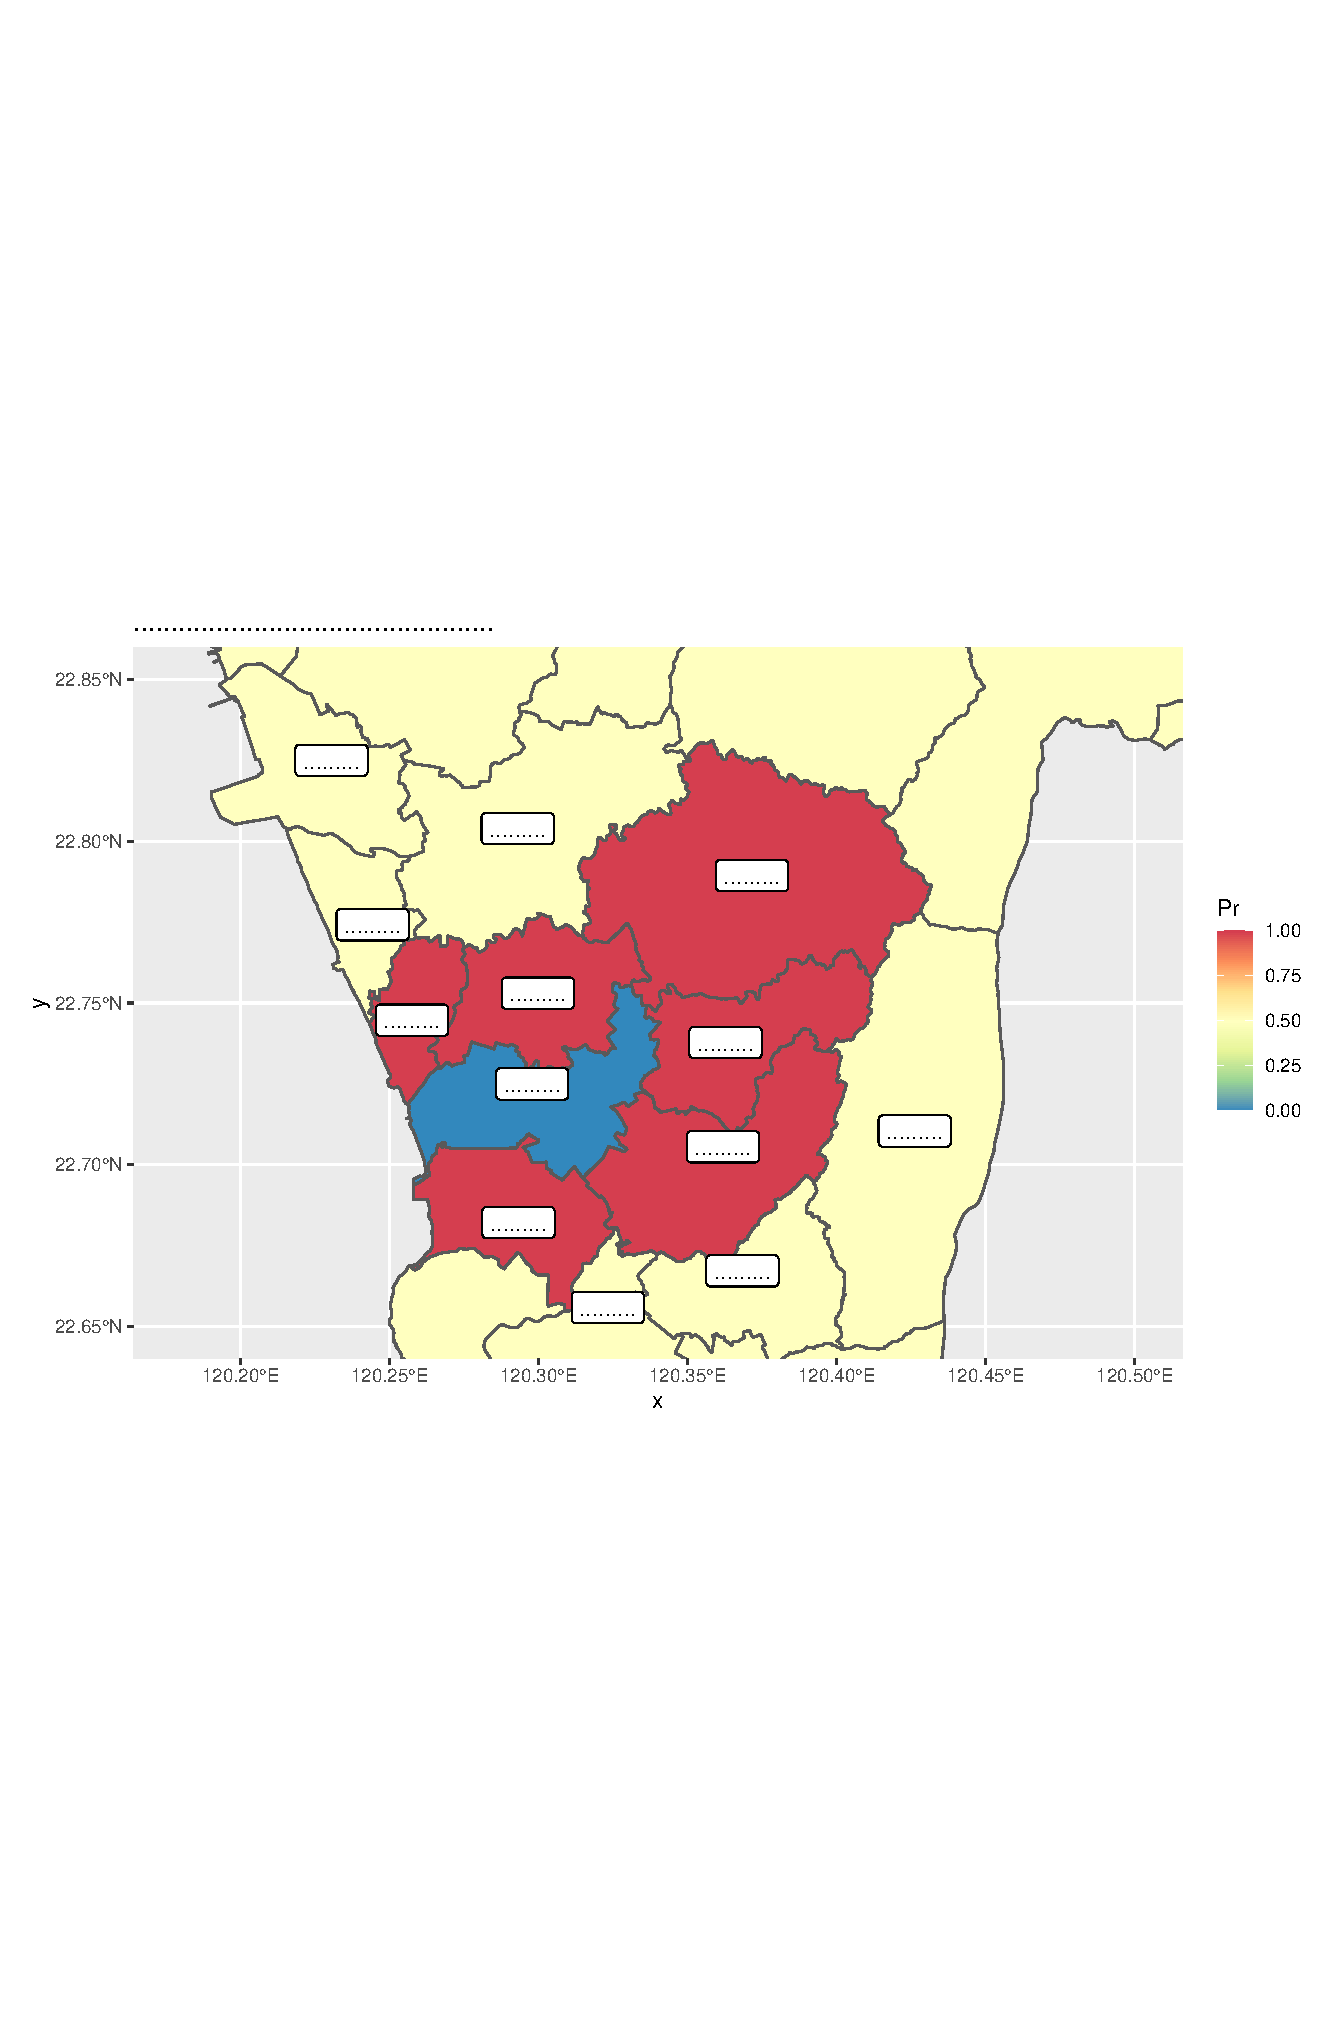
\includegraphics[width=0.7\textwidth]{example_C}
\caption{楠梓區與周圍邊界相鄰行政區關係圖}
\label{Fig.main3}
\end{figure}
\noindent

本論文嘗試採用 Chen 等人於 2006 年提出的基於M-H演算法的改善方法,該方法考慮到參數的後驗相關性,提高了MCMC的效率,加快了收斂速度。然而,在實際操作中,發現參數的更新導致交換率過低的問題,因此最終選擇不予採用該方法。完整的流程與結果收錄於附錄中。

%----------------------------------------------------------------------------------------------------------
\subsection{效果比較}\label{sec:4.2}
我們選用 Lambert (1992) 提出的零膨脹模型作為比較對象,並以 MLE 參數估計,同時, Lambert 的零膨脹模型並未考慮資料在時間與空間上的相關性。
與之相對的,本研究在此處的實驗將提出的模型在分位數 $\tau$ 設定為 0.5 之下計算參數估計結果,用以了解所提出的模型對比 Lambert 的模型在處理具有時間與空間相關性的資料時,分析效果是否更好。

 \setlength\abovedisplayskip{25pt}
 \setlength\belowdisplayskip{25pt}
由於模型平均為 $\left(1-p_i\right) \lambda_{ti}$,我們將透過 MCMC 生成的後驗樣本所估計而得的參數結果用以下公式求得反應變數估計值 $\hat{Y_{ti}}$ ,並以此計算 MSE,其中 $B$ 為所選取的近似獨立的後驗樣本個數, $med(\cdot)$ 表示 $B$ 個後驗樣本的中位數:
\begin{gather*}
\hat{\lambda}_{ti} = e^{\bm{X_{ti}^\prime}med(\bm{\beta}^{(1)},\ldots,\bm{\beta}^{(B)})+med(\delta^{(1)}_{ti},\ldots,\delta^{(B)}_{ti})}, \\[5mm]
\hat{p}_i = \frac{1}{1+e^{-(\bm{W_i^\prime}med(\bm{\alpha}^{(1)},\ldots,\bm{\alpha}^{(B)})+med(\sigma^{(1)}_R,\ldots,\sigma^{(B)}_R)(\zeta med(z^{(1)}_i,\ldots,z^{(B)}_i)+\xi \sqrt[]{med(z^{(1)}_i,\ldots,z^{(B)}_i)} med(u^{(1)}_i,\ldots,u^{(B)}_i)))}} \\[5mm]
\hat{Y}_{ti} = \left(1-\hat{p}_i\right)\hat{\lambda}_{ti}; \\[5mm]
t = 1,\dots,20, i = 1,\dots,38.
\end{gather*}

 \setlength\abovedisplayskip{25pt}
 \setlength\belowdisplayskip{25pt}
\noindent
MSE 計算公式:
\begin{gather*}
 MSE(\hat{Y})=\frac{1}{20\times 38}\sum_{t=1}^{20}\sum_{i=1}^{38}\left(\hat{Y}_{ti}-Y_{ti}\right)^2,
\end{gather*}
與上方公式相似, Lambert 模型的 MSE 計算方式只需將 $\hat{Y}_{ti}$ 帶入 Lambert 模型的預測值即可。
\begin{table}[H]
\centering
\setlength{\belowcaptionskip}{0.5cm}
\caption{Lambert (1992) 模型以最大概似估計法之迴歸係數估計結果}
\begin{tabular}{cccccc}
\hline
\multicolumn{6}{c}{Zero-inflation model coefficients (binomial with logit link):}\\
Estimate & Std.& Error & \emph{Z} Value & $Pr(>|z|)$\\
\hline
(Intercept) &-1.102 & 0.418 & -2.636 & 0.00838 & ** \\
經度 & -2.142 & 1.808 & -1.185 & 0.23601 &  \\
緯度 & 4.890 & 1.217 & 4.018 & $5.87\times10^{-5}$ & ***\\
每人分得的警政單位個數 & 6.087 & 3.990 & 1.526 & 0.127 &  \\
\hline
\hline
\multicolumn{6}{c}{Count model coefficients (poisson with log link):}\\
Estimate & Std.& Error & \emph{Z} Value & $Pr(>|z|)$\\
\hline
(Intercept) & 1.177 & 0.311 & 3.780 & 0.000157 & ***\\
部分刑事案件發生數 & 0.424 & 0.683 & 0.621 & 0.534456 & \\
低收入戶人數 & 1.842 & 0.902 & 2.042 & 0.041182 & *\\
離婚率 & 2.396 & 1.114 & 2.152 & 0.031437 & *\\
性別比 & -6.844 & 0.545 & -12.567 & $< 2\times10^{-16}$ & ***\\
\hline
\end{tabular}
\label{tab:3}
\end{table}
\noindent

表  \ref{tab:3} 的上半部分為零膨脹卜瓦松模型中結構零 $p$ 的迴歸係數估計結果,下半部分則是發生率 $\lambda$ 的迴歸係數估計結果。
結果顯示區公所的所在地的緯度對高雄市吸食快樂丸案件的發生與否具有顯著影響,並且迴歸係數為正,我們可以將其解釋為緯度越高,吸食快樂丸案件發生的可能性越低;
吸食快樂丸案件發生率的部分則是性別比具有顯著影響,迴歸係數為負,可以將其解釋為男性比例越高,吸食快樂丸案件發生率越低,
解釋變數低收入戶人數和離婚率則是顯著度較低。

在模型 (\ref{2}),本研究採用圖  \ref{Fig.main1} 所示之流程對模型參數與隨機效應項進行更新,並且根據 $\bm{\beta}$ 的蹤跡圖 (trace plot),在扣除前兩千次 MCMC 的結果後, $\bm{\beta}$ 呈現在一區間穩定跳動的收斂趨勢,因此將 MCMC 所取得的後驗樣本中的前兩千筆捨棄,使用 ACF 決定剩餘樣本取樣間隔,選取 ACF 中關聯性較低的值作為間隔多少取一次樣本的依據。
由於模型參數及隨機效應項眾多,本研究以聯合後驗分配,即公式 \eqref{10} ,的 ACF 圖做為間隔選取的依據。
\begin{figure}[H]
\centering
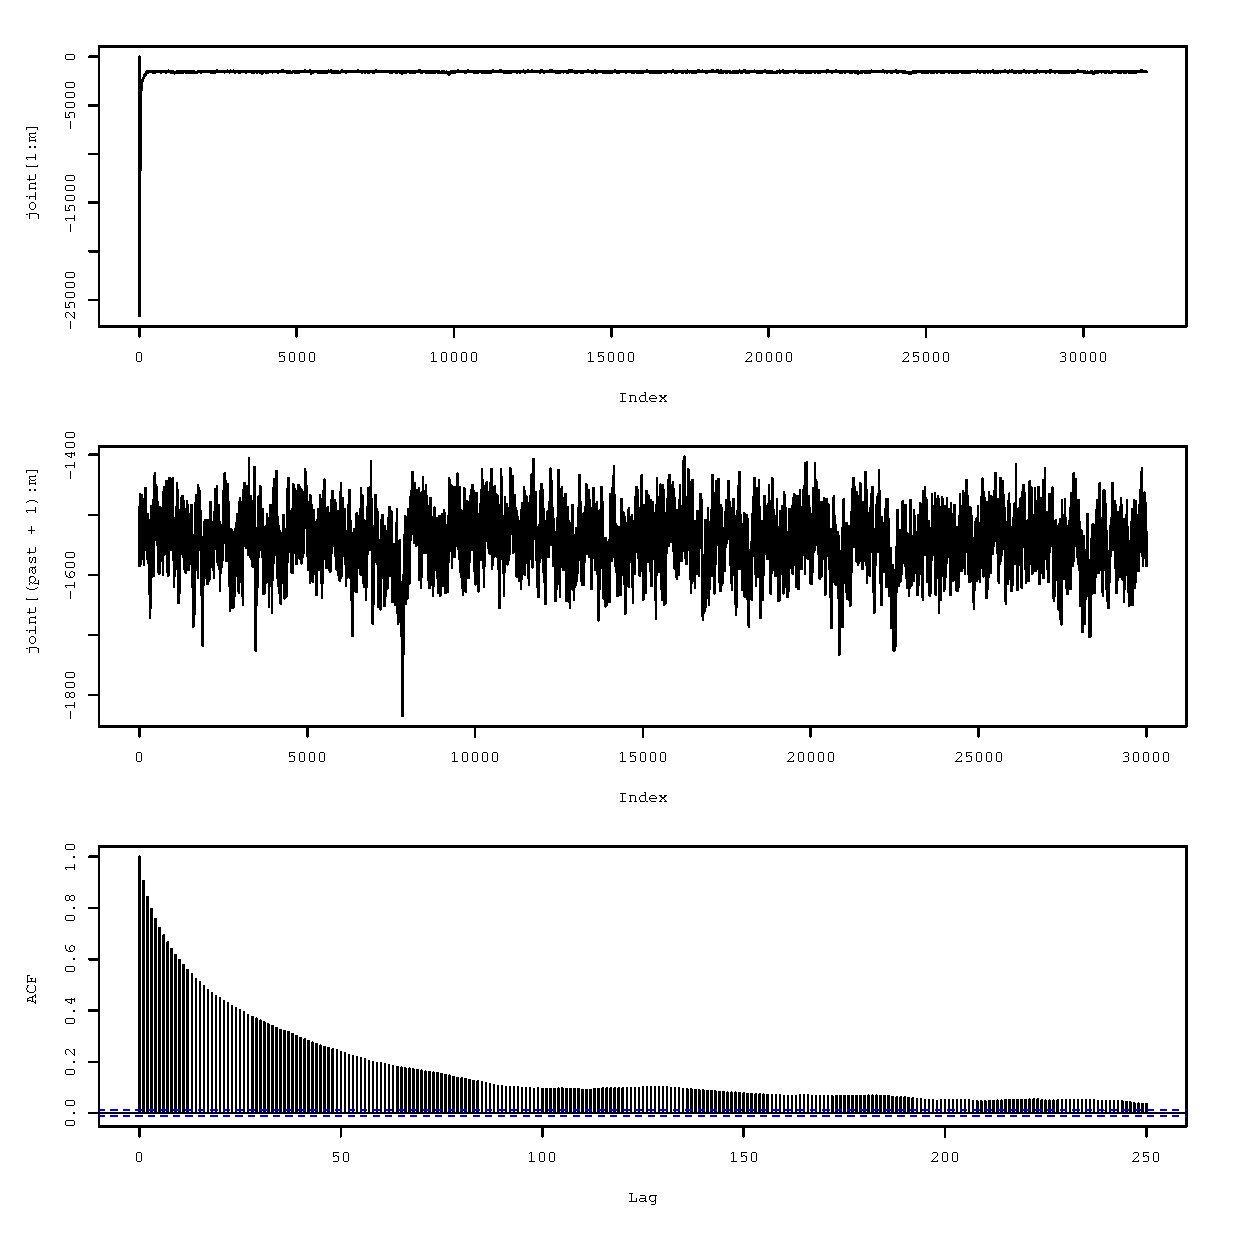
\includegraphics[width=1\textwidth]{joint.eps}
\caption{由上到下依序為聯合後驗分配的密度函數  \eqref{10} 蹤跡圖 (trace plot);預燒前 500 筆的聯合後驗分配的密度函數蹤跡圖 ;聯合後驗分配的密度函數 ACF 圖}
\label{Fig.main6}
\end{figure}
%\noindent
圖 \ref{Fig.main6} 中最上層兩張子圖依序分別為聯合後驗分配的密度函數蹤跡圖、以及預燒 (burn-in) 前 500 筆的聯合後驗分配的密度函數蹤跡圖,可以看到在扣除前 500 次的 MCMC 結果後,聯合後驗分配的密度函數呈現在一區間穩定跳動的趨勢,因此我們認為基於目前設定之下、此 MCMC 流程已達到穩定態;另外,圖 \ref{Fig.main6} 中最下層子圖為聯合後驗分配的密度函數 ACF 圖,其數值越小表示關聯性越小,透過 ACF 圖我們決定將剩餘的後驗樣本以間隔 300 次做一次樣本選取,最終取得 100 筆近似獨立的後驗樣本 (即 $b=1,\dots,100$)。

\begin{figure}[H]
\centering
\includegraphics[width=1\textwidth]{alpha_traceplot.eps}
\caption{$\bm{\alpha}$ 的蹤跡圖}
\label{Fig.main4}
\end{figure}
%\noindent
圖  \ref{Fig.main4} 為迴歸係數 $\bm{\alpha}$ 的蹤跡圖,由上到下分別對應常數項、各區區公所所在地的經度和緯度、各行政區每人分得的警政單位個數,可以看到 $\alpha_0$ 和 $\alpha_1$ 在兩萬次迭代前呈現漸減趨勢,後續逐漸平緩,而 $\alpha_3$ 則是相反,在兩萬次迭代前呈現漸增趨勢,並在約兩萬兩千後逐漸平緩,$\alpha_0,\alpha_1,\alpha_2,\alpha_3$ 的交換率皆為 0.99。

\begin{figure}[H]
\centering
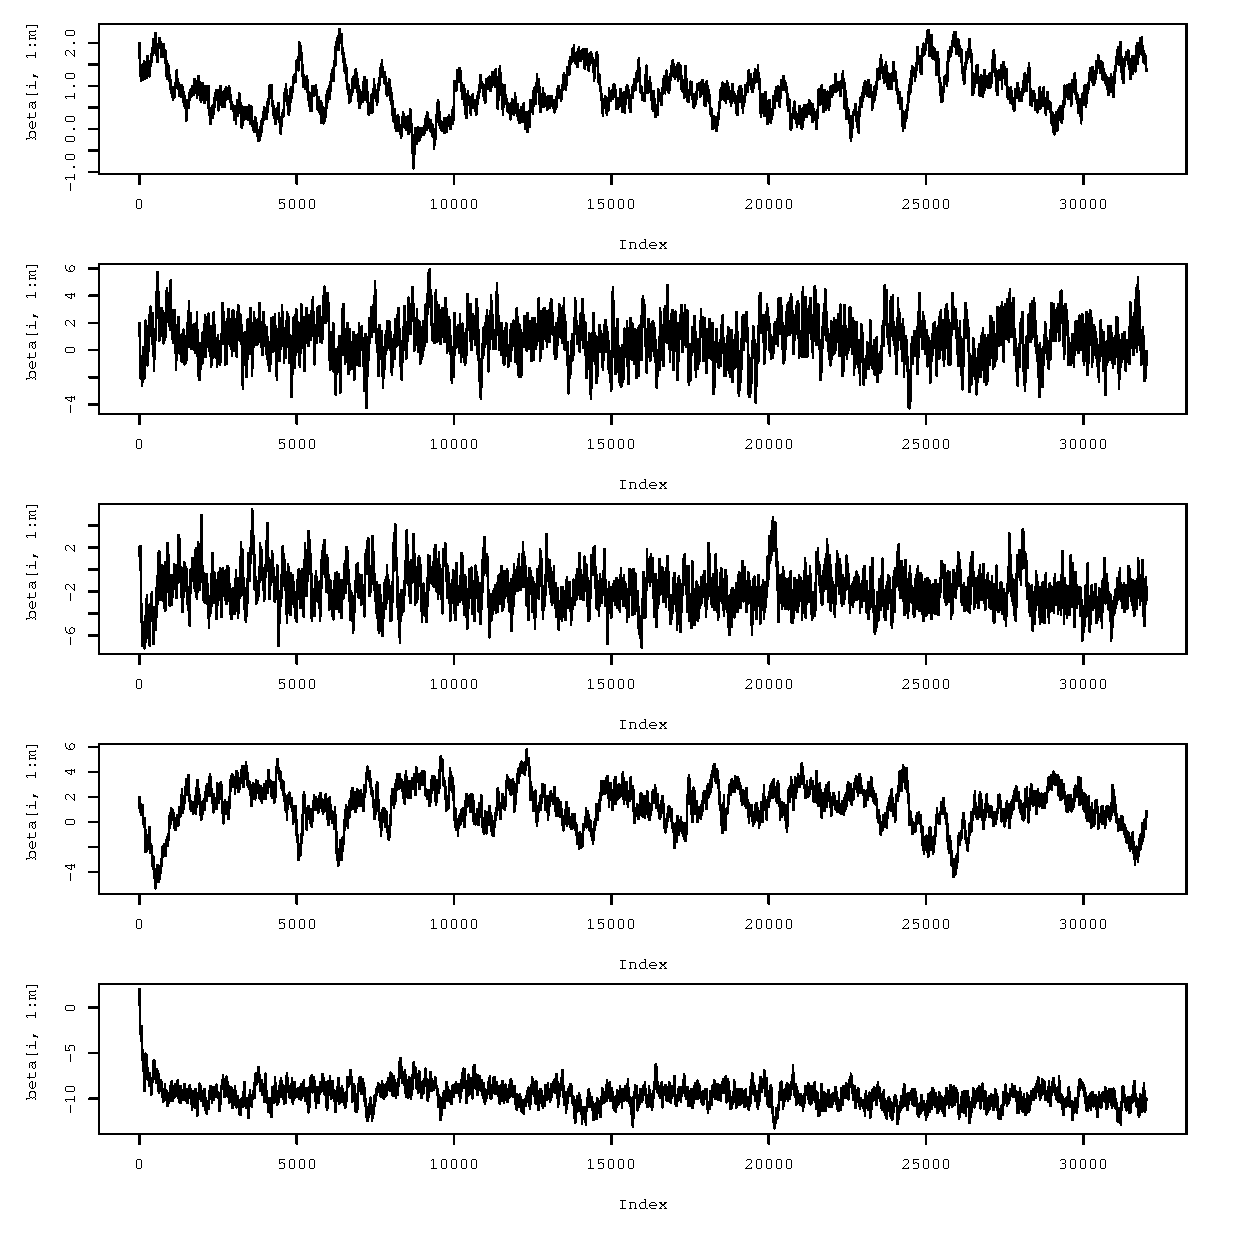
\includegraphics[width=1\textwidth]{beta_traceplot.eps}
\caption{$\bm{\beta}$ 的蹤跡圖}
\label{Fig.main5}
\end{figure}
%\noindent
圖 \ref{Fig.main5} 為迴歸係數 $\bm{\beta}$ 的蹤跡圖,由上到下分別對應常數項、部分刑事案件發生率、低收入戶人數比例、離婚率和性別比,可以看到 $\bm{\beta}$ 大致落在固定區間內,呈現收斂趨勢,並且 $\beta_0,\beta_1,\beta_2,\beta_3,\beta_4$ 的交換率分別為 0.46, 0.65, 0.72, 0.52, 0.47。

當 MSE 值較低表示模型計算出的反應變數估計 $\hat{Y}_{ti}$ 值更接近收集到的反應變數 $Y_{ti}$,模型估計結果更好。
本研究提出的模型 MSE 為 0.182,比較對象 Lambert 模型使用 MLE 參數估計的 MSE 為 1.707,顯示出本研究的模型的反應變數預測值比 Lambert 模型的預測值更接近真實值。



%----------------------------------------------------------------------------------------------------------
\subsection{分析結果}\label{sec:4.3}
本論文分別使用百分位數 $\tau =$ 0.25 、 0.5 、 0.75 代入模型以了解混合機率的分配情形,以 \ref{sec:2.2.3} 節的 MCMC 流程對參數進行更新,根據 ACF 圖決定參數選取間隔,最後得到 $B$ 組近似獨立的後驗樣本,並以此計算各參數後驗樣本的平均數、變異數、中位數、 2.5\% 及 97.5\% 百分位數。其中,當 2.5\% 和 97.5\% 百分位數間沒有包含零值時,我們將迴歸係數認定為顯著的,並在表 \ref{tab:4} 到表 \ref{tab:6} 中以星號標記。

表 \ref{tab:4} 到表 \ref{tab:6}分別在$\tau =$ 0.25 、 0.5 、 0.75 之下,記錄了結構零 $p_i$ 的迴歸係數 $\bm{\alpha}$ 和 $\lambda_{ti}$ 的迴歸係數 $\bm{\beta}$,$\alpha_0$ 為常數項, $\alpha_1$ 和 $\alpha_2$ 分別為各區區公所所在地的經度和緯度的迴歸係數,$\alpha_3$ 則對應到各行政區每人分得的警政單位個數;$\beta_0$ 同樣為常數項,$\beta_1$ 為部分刑事案件發生率,$\beta_2$ 則是低收入戶人數比例,$\beta_3$ 和 $\beta_4$ 分別對應離婚率和性別比。

首先,表 \ref{tab:4} 為 $\tau = 0.25$ 的迴歸係數估計結果。
可以看到迴歸係數 $\bm{\alpha}$ 僅有常數項和每人分得的警政單位個數 $\alpha_3$ 是顯著的,可以理解為每人分得的警政單位個數越多,則發生吸食快樂丸案件數的機率越低; $\bm{\beta}$ 則是只有 $\beta_4$ 性別比為負顯著,可以解釋為性別比愈高,快樂丸吸食人數愈低。
為了避免受到極端值影響,我們觀察在此分位數下的空間相關性參數 $\phi_t$ 的中位數以了解在不同時間下各行政區的空間相關性。對於所有 $\phi_t$ ; $t=1,\dots,20$ ,最大值為 0.169 ,最小值為 0.079。
接著,表 \ref{tab:5} 紀錄了 $\tau = 0.5$ 之下迴歸係數的估計結果,並且以此估計結果和 Lambert 模型的估計結果做 MSE 比較,如 \ref{sec:4.2} 節結果。
分位數 $\tau$ 改為 0.5 後,先前區公所所在地經度的迴歸係數 $\alpha_1$ 由不顯著變為顯著的, $\bm{\beta}$ 的部分顯著度則是常數項轉為顯著, $\beta_4$ 性別比同樣為負顯著。
空間相關性參數 $\phi_t$ 最大值為第十九期的 0.180 ,最小值為第十六期的 0.074 ,並且在 $\tau$ 為 0.25 之下空間相關性較低的期數與 $\tau$ 為 0.5 的結果相近。
最後,表 \ref{tab:6} 為 $\tau = 0.75$ 的估計結果,整體結果與 $\tau = 0.25$ 的結果相同,迴歸係數 $\alpha_2$ 為不顯著,其餘迴歸係數皆是顯著的;$\bm{\beta}$ 的部分除了先前不顯著的迴歸係數保持不變,常數項 $\beta_0$ 由顯著變為不顯著,僅剩性別比 $\beta_4$ 為顯著,並且 $\phi_t$ 最大值為 0.176 ,最小值為 0.082 ,空間相關性較低的期數同樣與先前兩個百分位數的結果相近。由於在百分位數 $\tau =$ 0.25 、 0.5 、 0.75 下的空間相關性參數結果相近,因此我們認為估計未受到極端值影響。
比較不同分位數之下的迴歸係數估計結果,區公所所在地的經度與各行政區每人分得警政單位個數在不同分位數下皆為顯著,因此推測以上兩個解釋變數對吸食快樂丸案件的發生與否具有顯著影響,發生率 $\lambda$ 的部分則是性別比具有顯著影響,並且與 Lambert 模型估計結果相同,迴歸係數為負,解釋為男性比例愈高,快樂丸案件發生率越低。我們推測背後的原因可能涉及國情的差異、不同毒品類別導致的結果差異,以及本次數據分析未納入重要的解釋變數。



\begin{table}
\centering
\setlength{\belowcaptionskip}{0.5cm}
\caption{$\tau$ 為 0.25 之下的迴歸係數估計結果}
\begin{tabular}{ccccccc}
\hline
& Mean & Std.& Median & 2.5\% & 97.5\% &\\
\hline
$\alpha_0$ & -0.691 & 0.164 & -0.623 & -1.579 & -0.079 & *\\
$\alpha_1$ & -0.235 & 0.063 & -0.250 & -0.713 &  0.271 &  \\
$\alpha_2$ & -1.088 & 1.155 & -1.575 & -2.390 &  0.651 &  \\
$\alpha_3$ &  1.773 & 0.351 &  1.658 &  0.511 &  2.663 & *\\
$\beta_0$  &  0.821 & 0.330 &  0.792 & -0.395 &  1.868 &  \\
$\beta_1$  &  0.737 & 3.232 &  0.840 & -2.924 &  4.020 &  \\
$\beta_2$  & -0.748 & 4.795 & -1.854 & -4.485 &  1.868 &  \\
$\beta_3$  &  0.987 & 3.178 &  0.977 & -2.177 &  4.374 &  \\
$\beta_4$  & -8.628 & 1.405 & -8.647 &-10.614 & -6.306 & *\\
\hline
$ \phi_1$   & 0.125 & 0.002 & 0.140 & 0.019 & 0.189 & \\
$ \phi_2$   & 0.109 & 0.002 & 0.119 & 0.012 & 0.187 & \\
$ \phi_3$   & 0.091 & 0.003 & 0.094 & 0.005 & 0.182 & \\
$ \phi_4$   & 0.101 & 0.004 & 0.106 & 0.004 & 0.174 & \\
$ \phi_5$   & 0.115 & 0.003 & 0.121 & 0.008 & 0.191 & \\
$ \phi_6$   & 0.089 & 0.003 & 0.088 & 0.003 & 0.182 & \\
$ \phi_7$   & 0.116 & 0.003 & 0.128 & 0.010 & 0.191 & \\
$ \phi_8$   & 0.095 & 0.003 & 0.089 & 0.016 & 0.179 & \\
$ \phi_9$   & 0.106 & 0.003 & 0.117 & 0.007 & 0.180 & \\
$\phi_{10}$ & 0.108 & 0.003 & 0.112 & 0.011 & 0.187 & \\
$\phi_{11}$ & 0.101 & 0.003 & 0.107 & 0.005 & 0.184 & \\
$\phi_{12}$ & 0.099 & 0.003 & 0.094 & 0.012 & 0.186 & \\
$\phi_{13}$ & 0.101 & 0.003 & 0.101 & 0.015 & 0.187 & \\
$\phi_{14}$ & 0.086 & 0.003 & 0.079 & 0.007 & 0.178 & \\
$\phi_{15}$ & 0.089 & 0.003 & 0.082 & 0.010 & 0.181 & \\
$\phi_{16}$ & 0.089 & 0.003 & 0.083 & 0.006 & 0.181 & \\
$\phi_{17}$ & 0.137 & 0.003 & 0.164 & 0.012 & 0.192 & \\
$\phi_{18}$ & 0.146 & 0.003 & 0.161 & 0.012 & 0.194 & \\
$\phi_{19}$ & 0.150 & 0.002 & 0.169 & 0.038 & 0.194 & \\
$\phi_{20}$ & 0.136 & 0.003 & 0.153 & 0.023 & 0.192 & \\
\hline
\end{tabular}
\label{tab:4}
\end{table}
\noindent
\begin{table}
\centering
\setlength{\belowcaptionskip}{0.5cm}
\caption{$\tau$ 為 0.5 之下的迴歸係數估計結果}
\begin{tabular}{ccccccc}
\hline
& Mean & Std.& Median & 2.5\% & 97.5\% &\\
\hline
$\alpha_0$ & -2.257 & 1.292 & -2.304 & -3.854 & -0.477 & *\\
$\alpha_1$ & -1.266 & 0.211 & -1.249 & -2.058 & -0.337 & *\\
$\alpha_2$ & -0.380 & 0.060 & -0.363 & -0.778 &  0.094 &  \\
$\alpha_3$ &  1.463 & 0.287 &  1.449 &  0.407 &  2.325 & *\\
$\beta_0$  &  0.864 & 0.247 &  0.808 &  0.034 &  1.816 & *\\
$\beta_1$  &  0.896 & 2.247 &  1.057 & -2.444 &  3.280 &  \\
$\beta_2$  & -1.935 & 2.346 & -2.162 & -4.738 &  1.224 &  \\
$\beta_3$  &  1.324 & 2.255 &  1.407 & -1.901 &  3.604 &  \\
$\beta_4$  & -9.587 & 1.168 & -9.606 &-11.479 & -7.410 & *\\
\hline
$ \phi_1$   & 0.139 & 0.002 & 0.157 & 0.025 & 0.193 & \\
$ \phi_2$   & 0.121 & 0.003 & 0.132 & 0.005 & 0.189 & \\
$ \phi_3$   & 0.109 & 0.003 & 0.124 & 0.008 & 0.187 & \\
$ \phi_4$   & 0.100 & 0.003 & 0.100 & 0.007 & 0.187 & \\
$ \phi_5$   & 0.112 & 0.003 & 0.121 & 0.017 & 0.187 & \\
$ \phi_6$   & 0.091 & 0.003 & 0.091 & 0.006 & 0.180 & \\
$ \phi_7$   & 0.109 & 0.003 & 0.121 & 0.009 & 0.188 & \\
$ \phi_8$   & 0.090 & 0.003 & 0.088 & 0.002 & 0.184 & \\
$ \phi_9$   & 0.114 & 0.002 & 0.121 & 0.013 & 0.189 & \\
$\phi_{10}$ & 0.101 & 0.003 & 0.113 & 0.013 & 0.187 & \\
$\phi_{11}$ & 0.104 & 0.003 & 0.112 & 0.007 & 0.180 & \\
$\phi_{12}$ & 0.106 & 0.003 & 0.104 & 0.015 & 0.186 & \\
$\phi_{13}$ & 0.095 & 0.003 & 0.095 & 0.003 & 0.190 & \\
$\phi_{14}$ & 0.092 & 0.003 & 0.091 & 0.006 & 0.183 & \\
$\phi_{15}$ & 0.089 & 0.003 & 0.090 & 0.005 & 0.180 & \\
$\phi_{16}$ & 0.084 & 0.003 & 0.074 & 0.004 & 0.182 & \\
$\phi_{17}$ & 0.148 & 0.002 & 0.165 & 0.016 & 0.194 & \\
$\phi_{18}$ & 0.133 & 0.003 & 0.154 & 0.014 & 0.191 & \\
$\phi_{19}$ & 0.155 & 0.002 & 0.180 & 0.036 & 0.194 & \\
$\phi_{20}$ & 0.137 & 0.002 & 0.154 & 0.036 & 0.192 & \\
\hline
\end{tabular}
\label{tab:5}
\end{table}
\noindent

\begin{table}
\centering
\setlength{\belowcaptionskip}{0.5cm}
\caption{$\tau$ 為 0.75 之下的迴歸係數估計結果}
\begin{tabular}{ccccccc}
\hline
& Mean & Std.& Median & 2.5\% & 97.5\% &\\
\hline
$\alpha_0$ & -1.974 & 0.468 & -1.993 & -3.259 & -0.714 & *\\
$\alpha_1$ & -0.073 & 0.103 &  0.097 & -0.690 &  0.459 &  \\
$\alpha_2$ & -0.663 & 0.134 & -0.728 & -1.226 &  0.042 &  \\
$\alpha_3$ &  0.811 & 0.222 &  0.803 &  0.106 &  1.656 & *\\
$\beta_0$  &  0.823 & 0.268 &  0.785 & -0.038 &  1.888 &  \\
$\beta_1$  &  0.399 & 2.526 &  0.477 & -2.764 &  3.480 &  \\
$\beta_2$  & -1.615 & 1.969 & -1.793 & -3.977 &  1.688 &  \\
$\beta_3$  &  1.610 & 2.866 &  1.715 & -1.833 &  4.576 &  \\
$\beta_4$  &-10.139 & 0.752 &-10.167 &-11.716 & -8.477 & *\\
\hline
$ \phi_1$   & 0.145 & 0.002 & 0.159 & 0.049 & 0.191 & \\
$ \phi_2$   & 0.119 & 0.003 & 0.133 & 0.014 & 0.189 & \\
$ \phi_3$   & 0.107 & 0.003 & 0.120 & 0.008 & 0.186 & \\
$ \phi_4$   & 0.106 & 0.003 & 0.113 & 0.007 & 0.185 & \\
$ \phi_5$   & 0.117 & 0.003 & 0.125 & 0.005 & 0.190 & \\
$ \phi_6$   & 0.086 & 0.003 & 0.087 & 0.003 & 0.184 & \\
$ \phi_7$   & 0.116 & 0.003 & 0.128 & 0.013 & 0.190 & \\
$ \phi_8$   & 0.087 & 0.003 & 0.083 & 0.011 & 0.176 & \\
$ \phi_9$   & 0.132 & 0.003 & 0.147 & 0.016 & 0.190 & \\
$\phi_{10}$ & 0.116 & 0.003 & 0.118 & 0.019 & 0.190 & \\
$\phi_{11}$ & 0.099 & 0.002 & 0.100 & 0.012 & 0.186 & \\
$\phi_{12}$ & 0.106 & 0.003 & 0.123 & 0.005 & 0.189 & \\
$\phi_{13}$ & 0.087 & 0.003 & 0.086 & 0.006 & 0.182 & \\
$\phi_{14}$ & 0.107 & 0.003 & 0.117 & 0.008 & 0.190 & \\
$\phi_{15}$ & 0.091 & 0.002 & 0.093 & 0.009 & 0.177 & \\
$\phi_{16}$ & 0.089 & 0.003 & 0.080 & 0.009 & 0.183 & \\
$\phi_{17}$ & 0.156 & 0.002 & 0.181 & 0.030 & 0.194 & \\
$\phi_{18}$ & 0.146 & 0.002 & 0.165 & 0.024 & 0.192 & \\
$\phi_{19}$ & 0.158 & 0.002 & 0.175 & 0.020 & 0.194 & \\
$\phi_{20}$ & 0.123 & 0.003 & 0.134 & 0.012 & 0.192 & \\

\hline
\end{tabular}
\label{tab:6}
\end{table}
\noindent


%----------------------------------------------------------------------------------------------------------
\subsection{風險比}\label{sec:4.4}

本論文提出以下 $R_i(t_1,t_2)$ 函數,比較區域 $A_i$ 在時間點 $t_1$ 和 $t_2$ 發生率比值,用以了解高雄各行政區連續兩季度間的發生率變化:
 \begin{gather*}
 R_i^{(b)}(t_1,t_2) = \frac{\lambda_{t_1i}^{(b)}}{\lambda_{t_2i}^{(b)}}, \\
 t_1 = 1,\dots,19;\:\:t_2 = t_1+1;\:\:i = 1,\dots,38;\:\:b = 1,\dots,100.
 \end{gather*}
\noindent
透過 MCMC 所生成各參數與隨機效應項的近似獨立後驗樣本,計算得到發生率 $\lambda_{ti}^{(b)}$ 與其比值 $R_i^{(b)}(t_1,t_2)$,進一步探討發生率風險的變化,以 $R_i^{(b)}(t_1,t_2) \mbox{,} b = 1,\dots,100$ 的樣本平均數逼近 $P(R_i(t_1,t_2) \ge 1|\bm{Y}_1,\dots,\bm{Y}_{20})$。
根據 $R_i^{(b)}(t_1,t_2)$ 的定義,我們可以將機率高解釋為吸食快樂丸案件發生率下降的可能性高,由此了解不同時間點的案件發生率變化。
資料共二十季,因此共有十九期風險機率圖,在後續圖 \ref{Fig.main5} 到圖 \ref{Fig.main10} 分別展示分位數 $\tau =$ 0.25 、 0.5 、 0.75 之下的風險機率圖做觀察。
可以看到在十九期風險機率圖中,並沒有出現長期呈現紅色或藍色,顯示案件發生率隨著時間呈現波動的情形,並且我們觀察到發生率上升的地區,其周邊地區發生率同樣呈現上升,我們可以理解為區域間互相影響,導致區域發生率升高。
因此我們認為可以將風險比用於評估區域發生率的變化趨勢,作為未來決策的判斷依據。
\\ \hspace*{\fill} \\
\begin{figure}[htpb]
\centering
\subfigure[第一期]{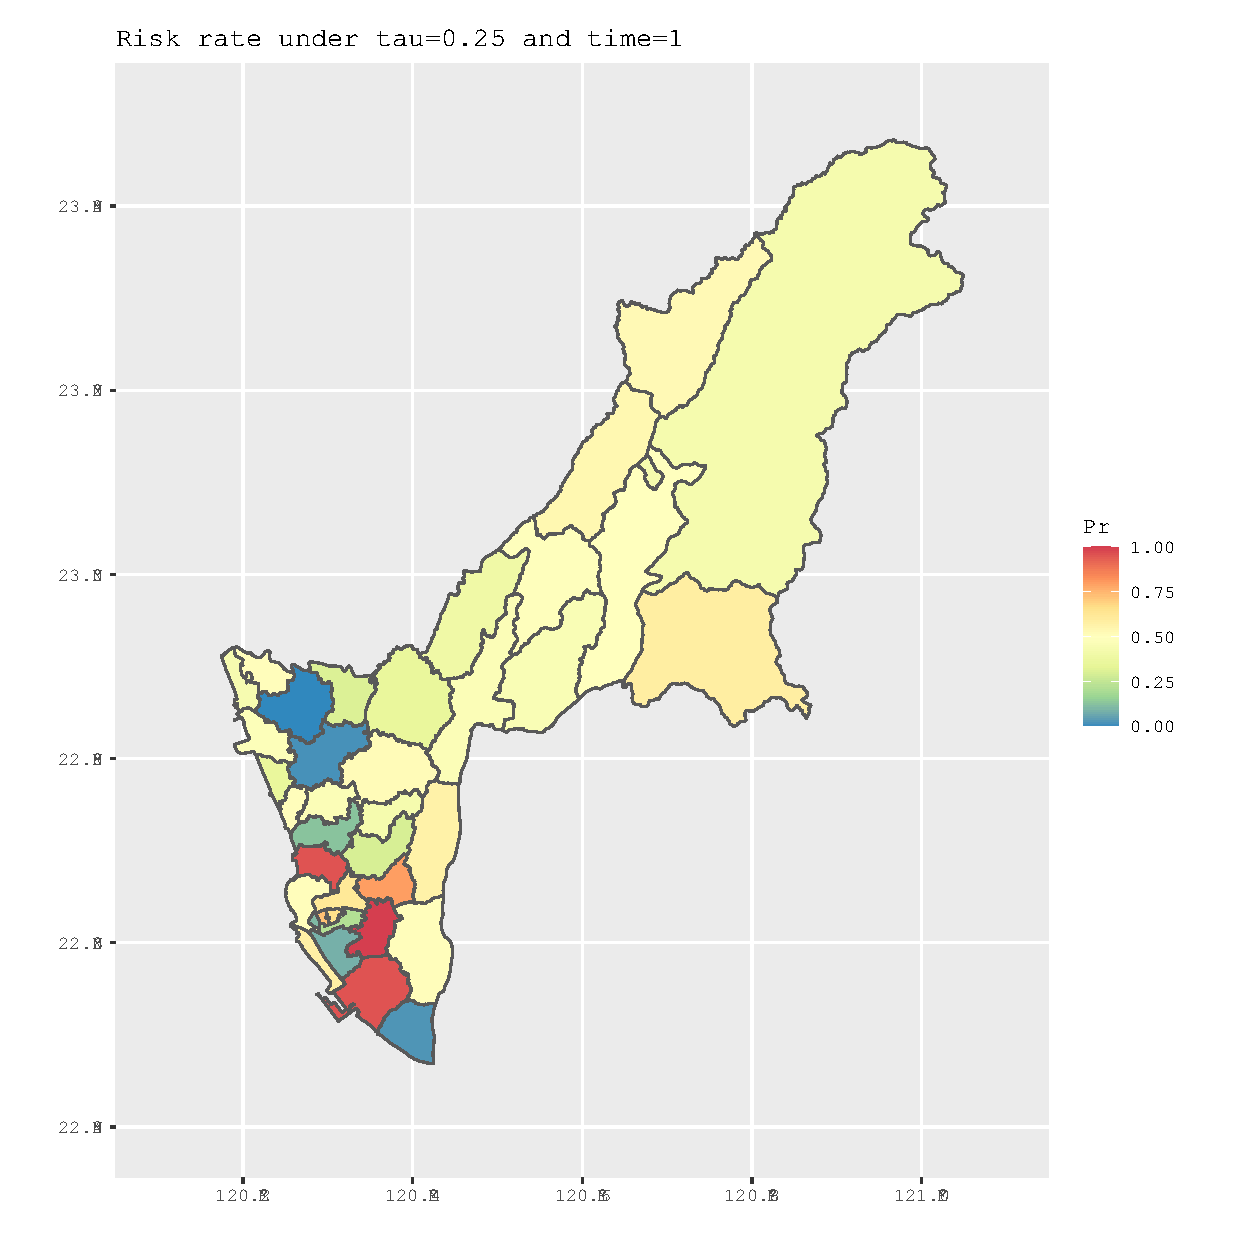
\includegraphics[width=0.22\paperwidth]{Risk_rate_under_tau=0.25_and_time=1.eps}}
\subfigure[第二期]{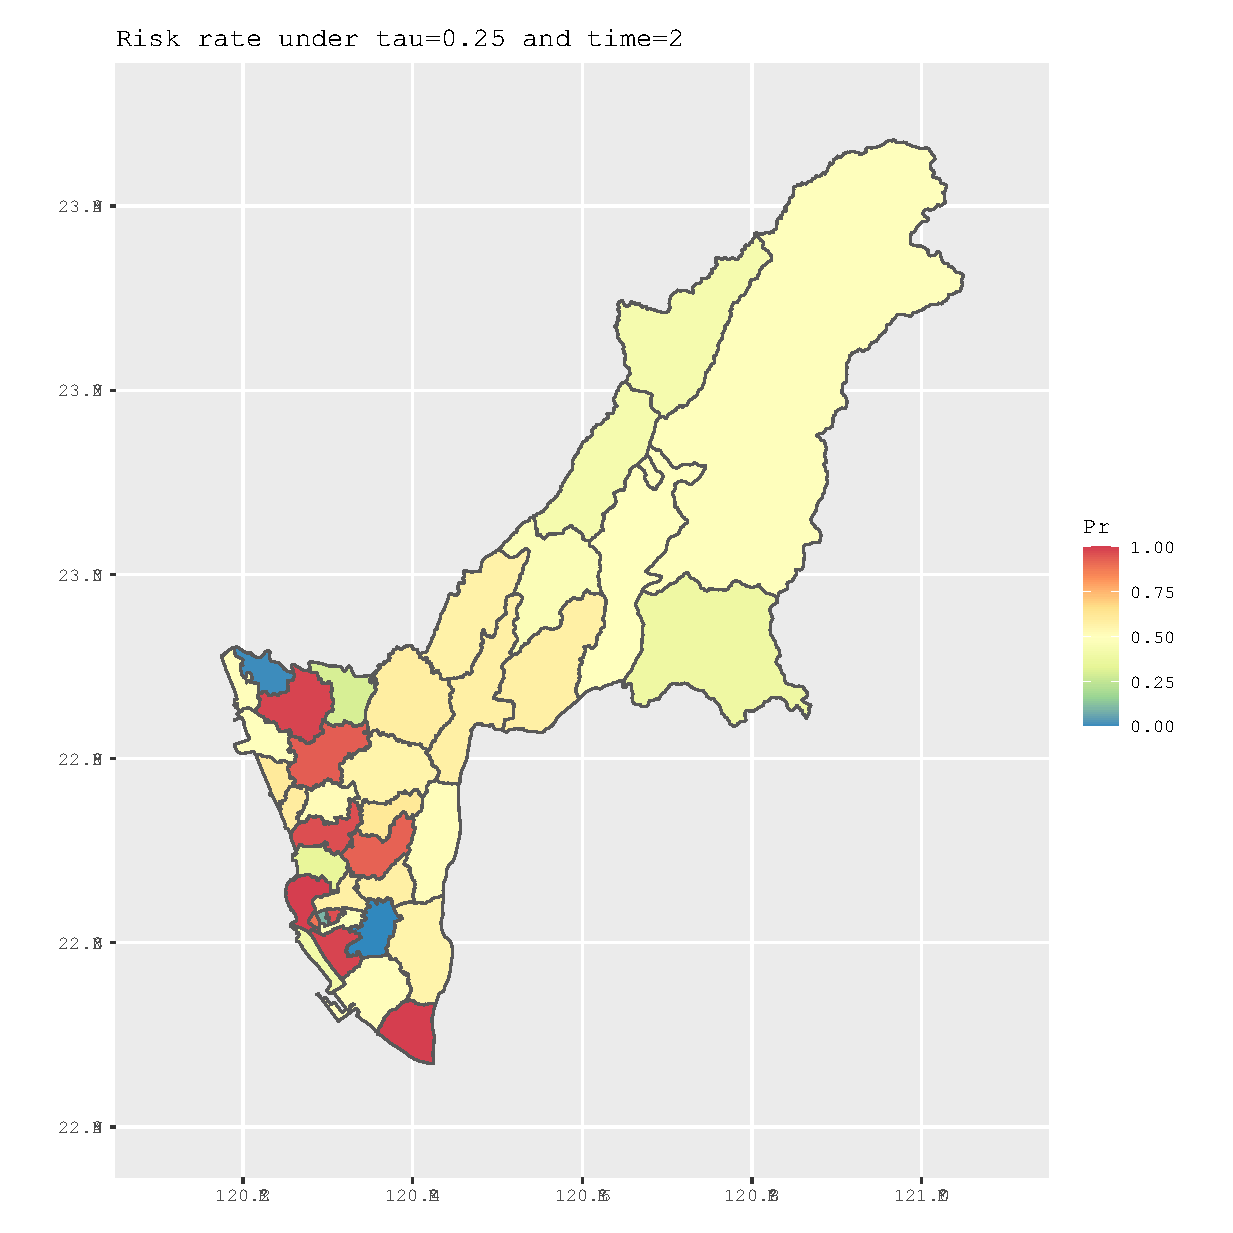
\includegraphics[width=0.22\paperwidth]{Risk_rate_under_tau=0.25_and_time=2.eps}}
\subfigure[第三期]{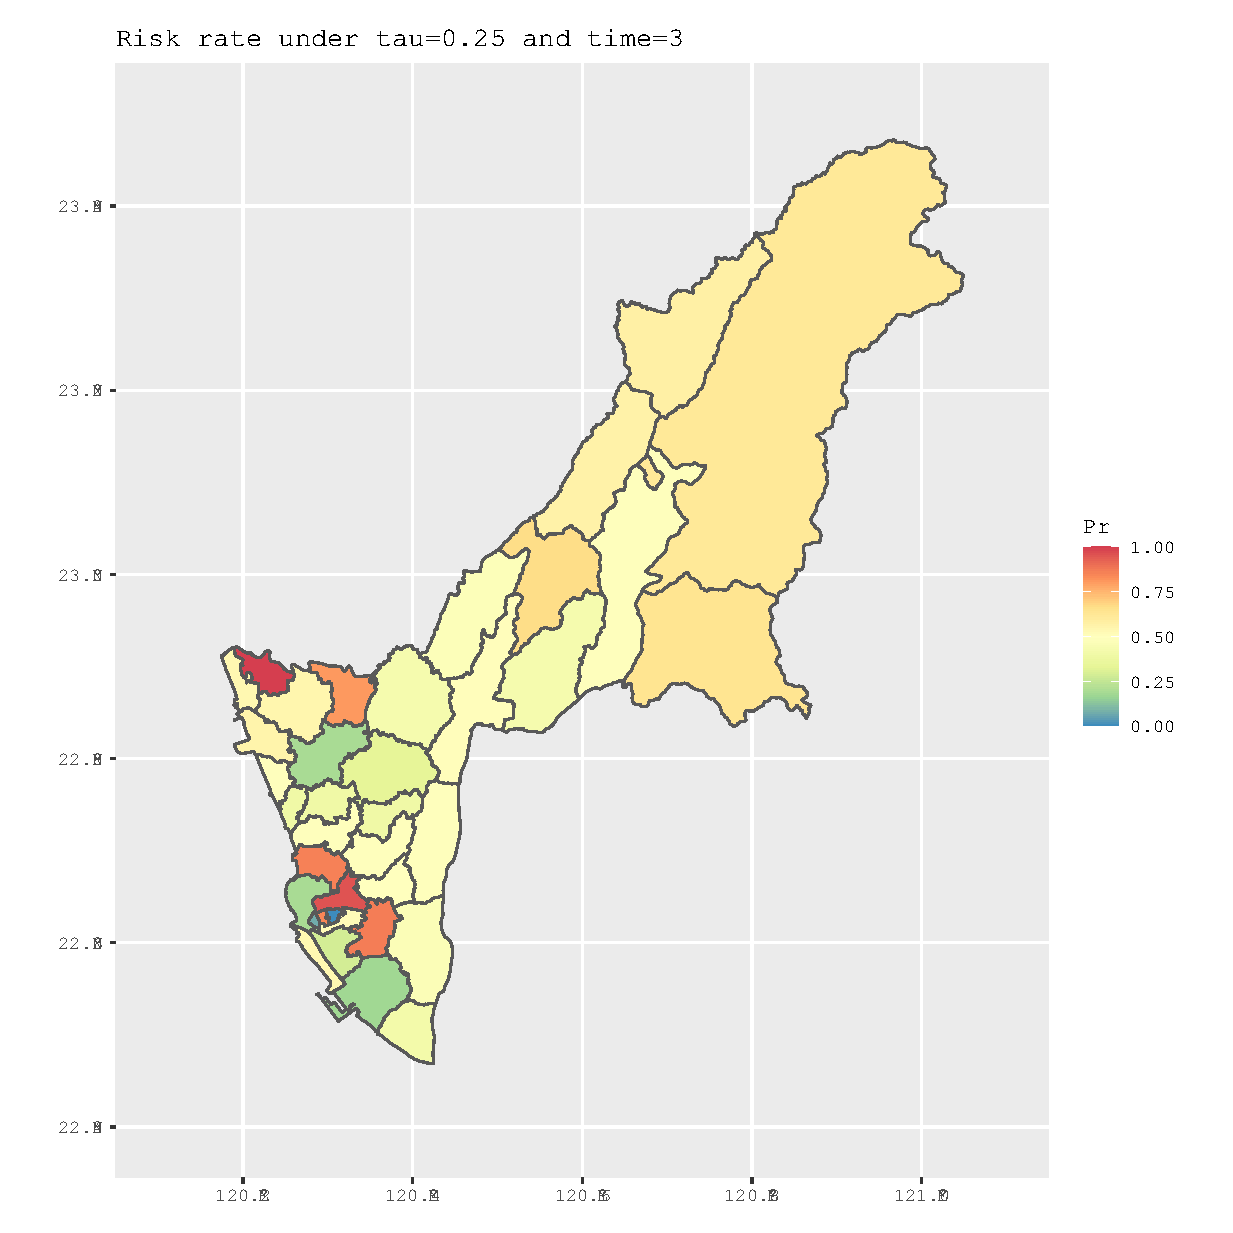
\includegraphics[width=0.22\paperwidth]{Risk_rate_under_tau=0.25_and_time=3.eps}} \\
\subfigure[第四期]{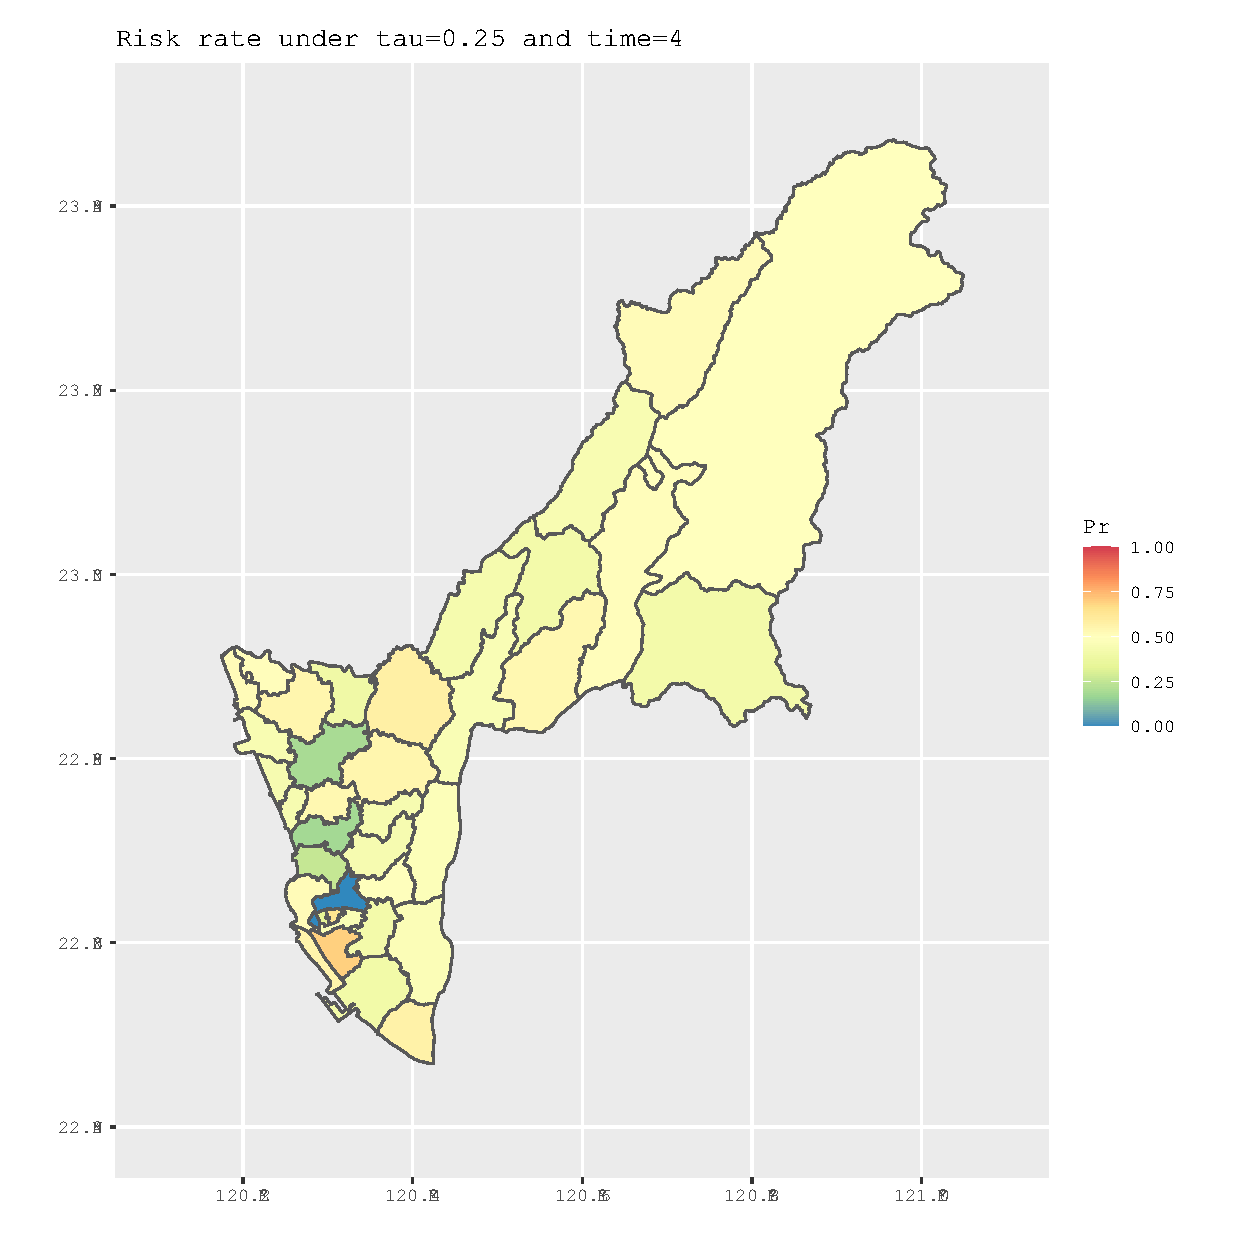
\includegraphics[width=0.22\paperwidth]{Risk_rate_under_tau=0.25_and_time=4.eps}}
\subfigure[第五期]{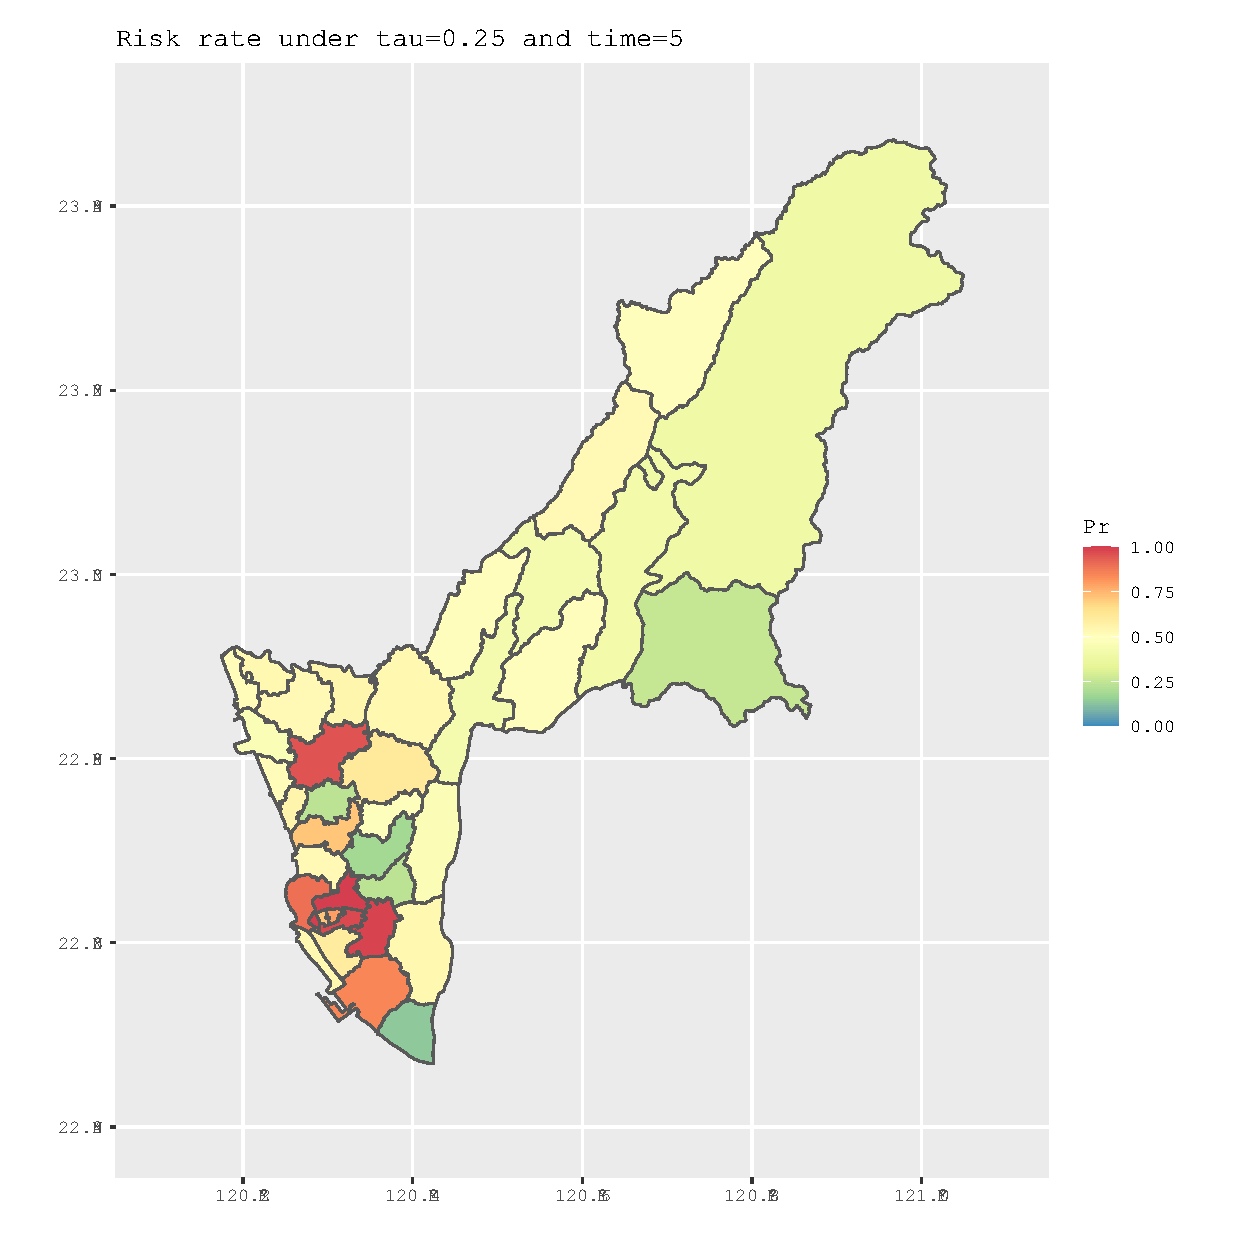
\includegraphics[width=0.22\paperwidth]{Risk_rate_under_tau=0.25_and_time=5.eps}}
\subfigure[第六期]{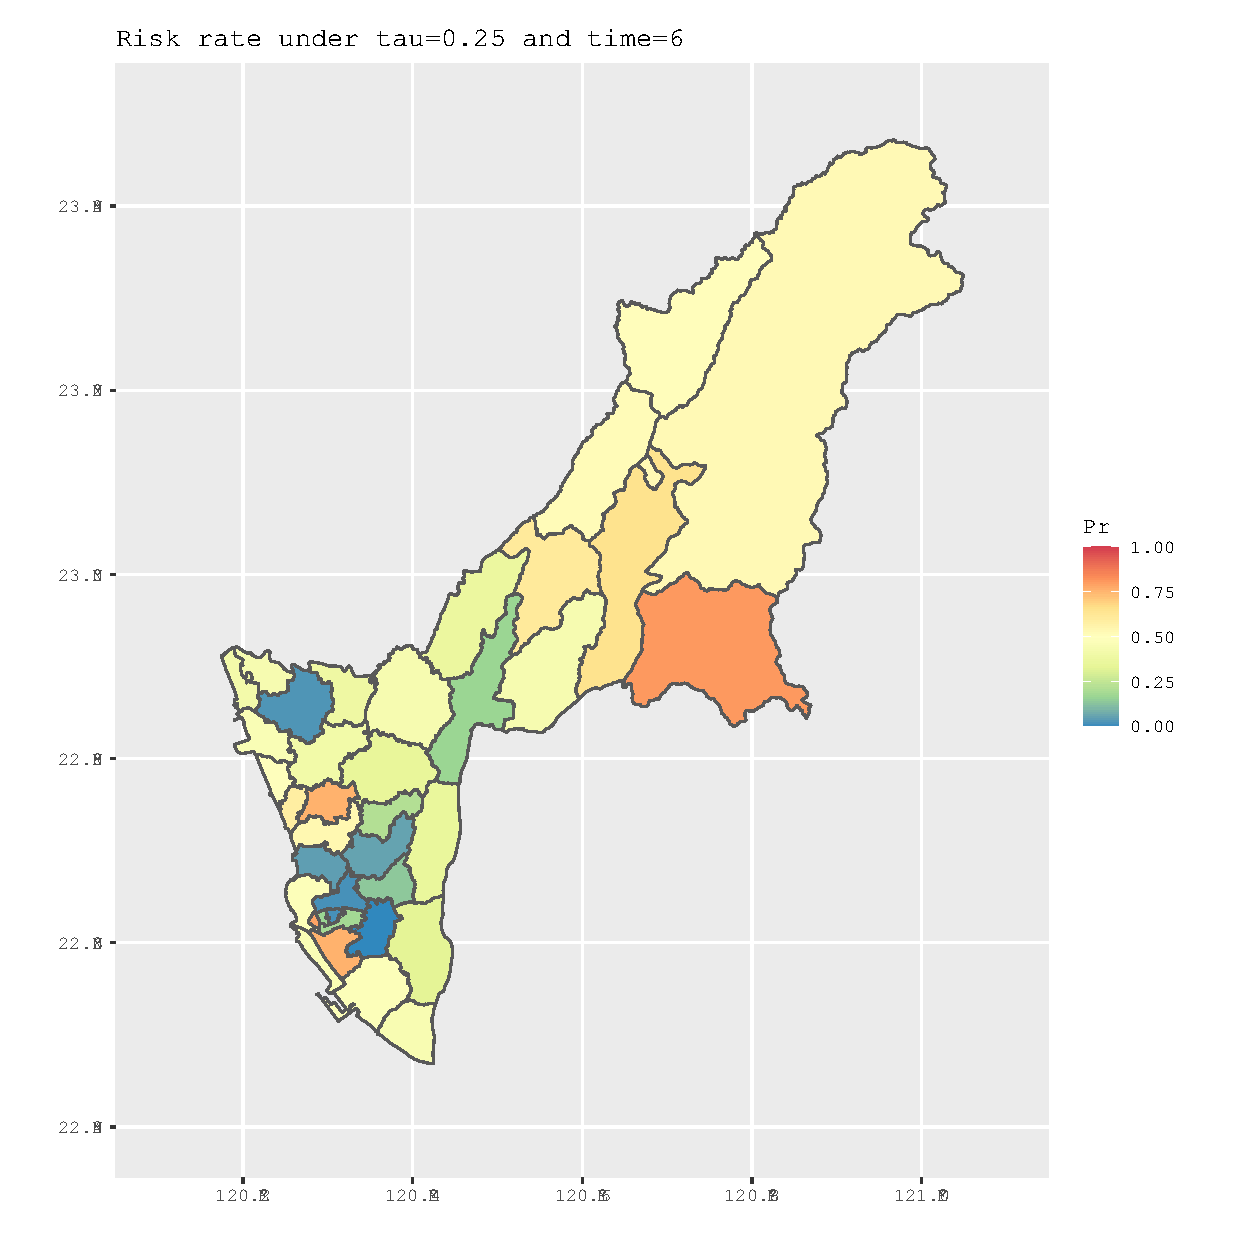
\includegraphics[width=0.22\paperwidth]{Risk_rate_under_tau=0.25_and_time=6.eps}} \\
\subfigure[第七期]{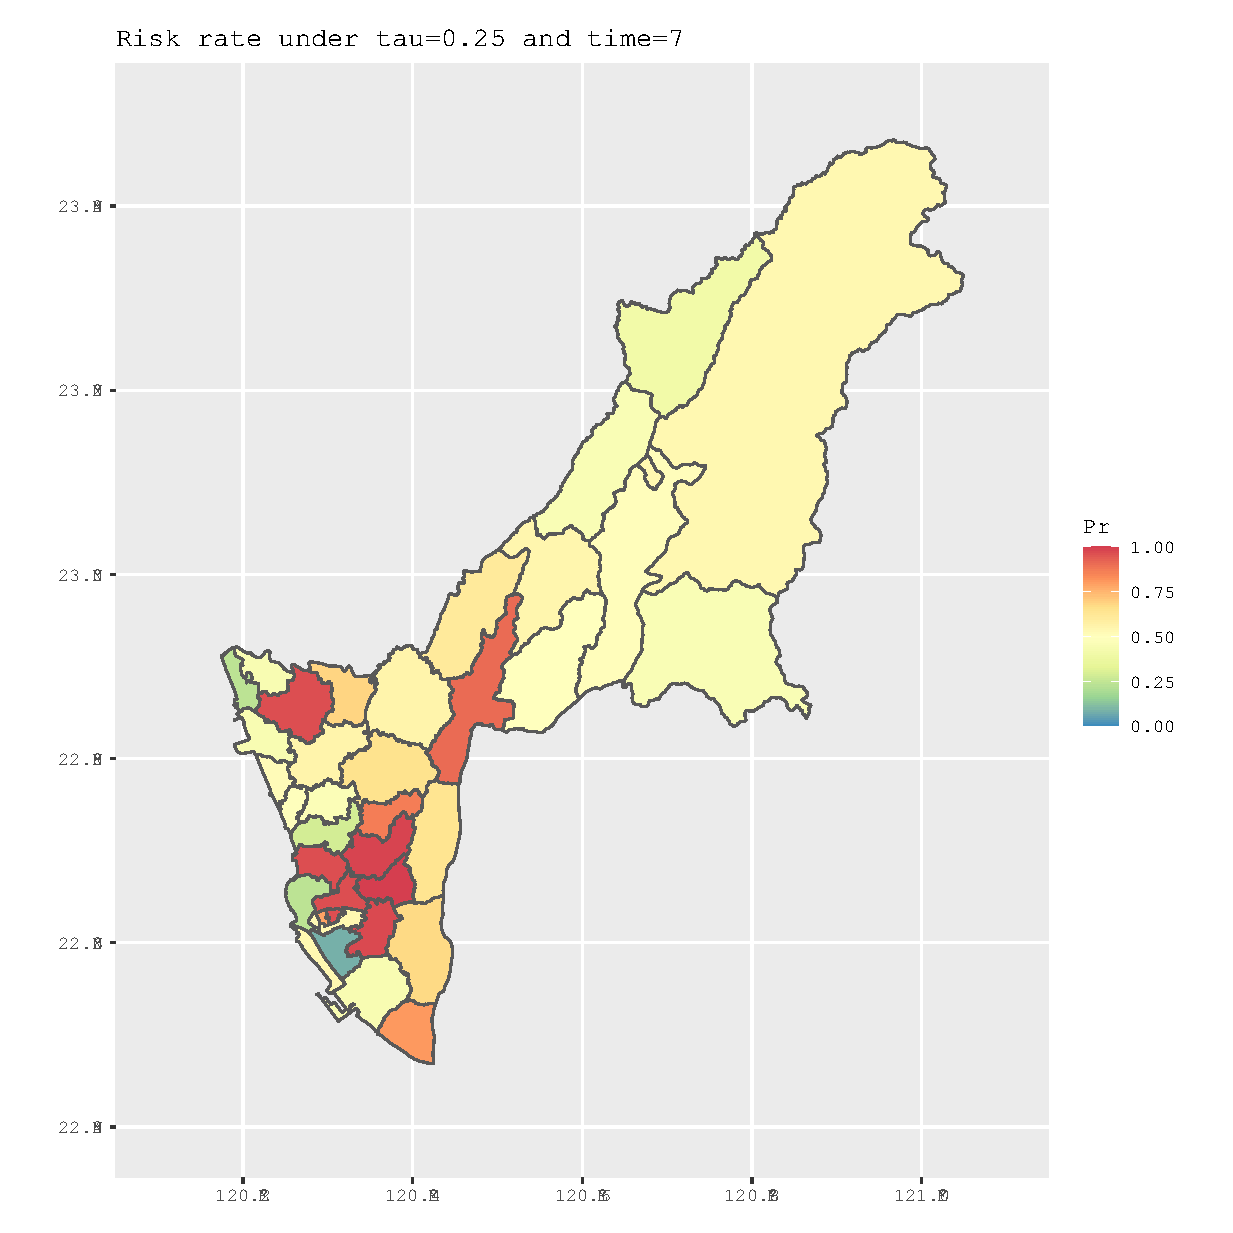
\includegraphics[width=0.22\paperwidth]{Risk_rate_under_tau=0.25_and_time=7.eps}}
\subfigure[第八期]{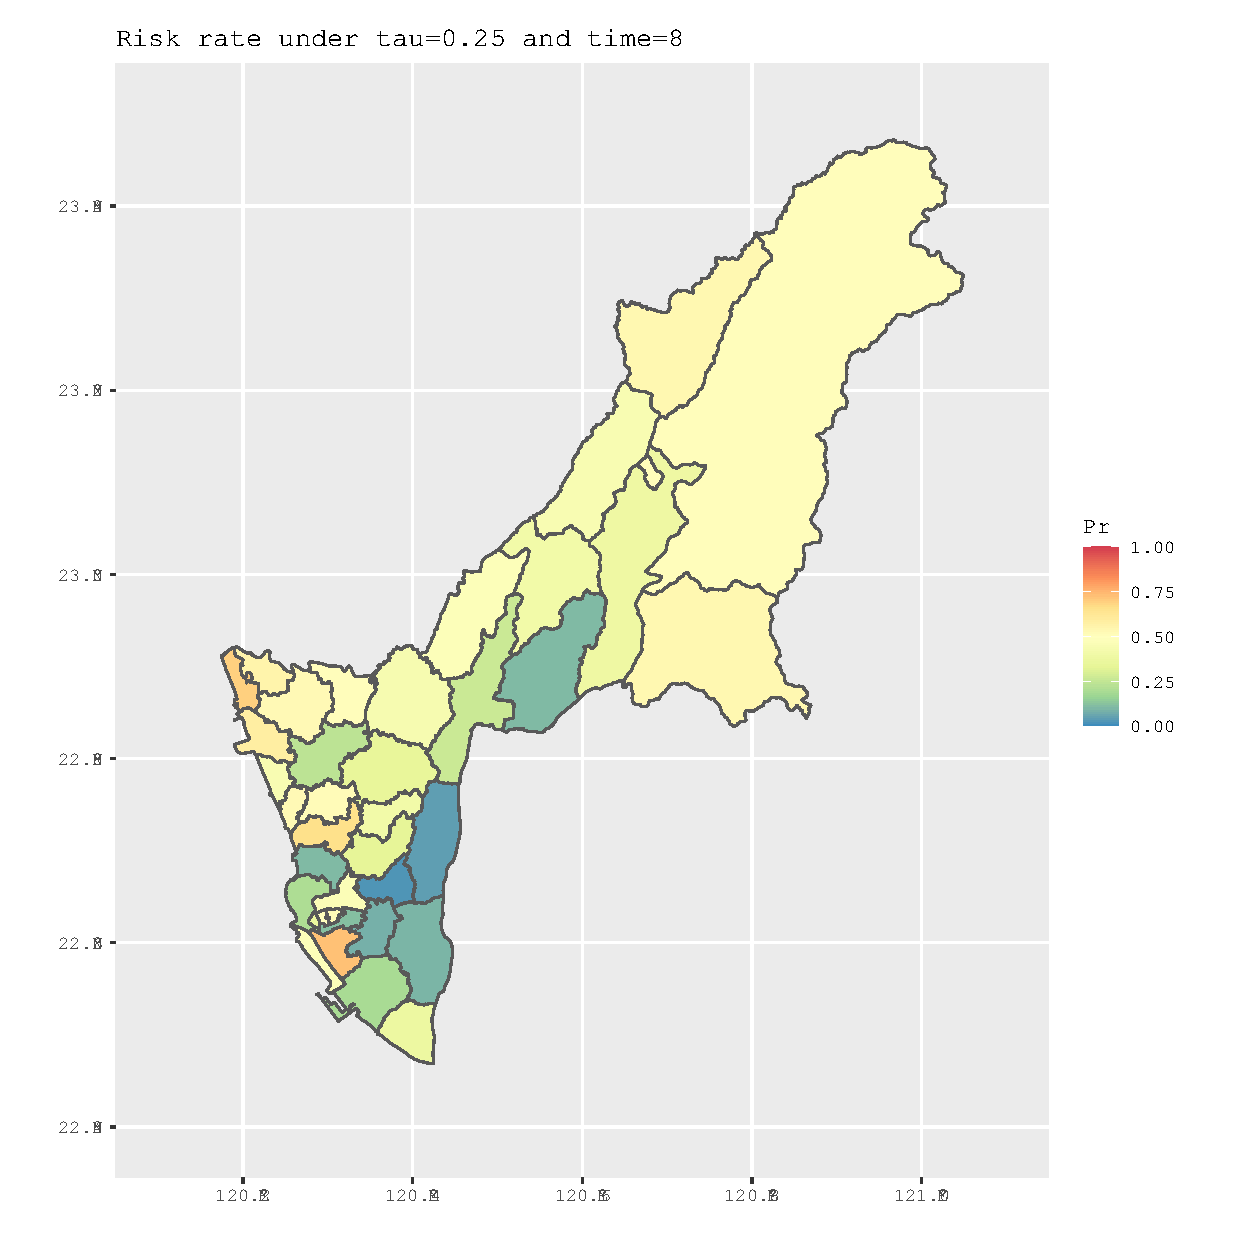
\includegraphics[width=0.22\paperwidth]{Risk_rate_under_tau=0.25_and_time=8.eps}}
\subfigure[第九期]{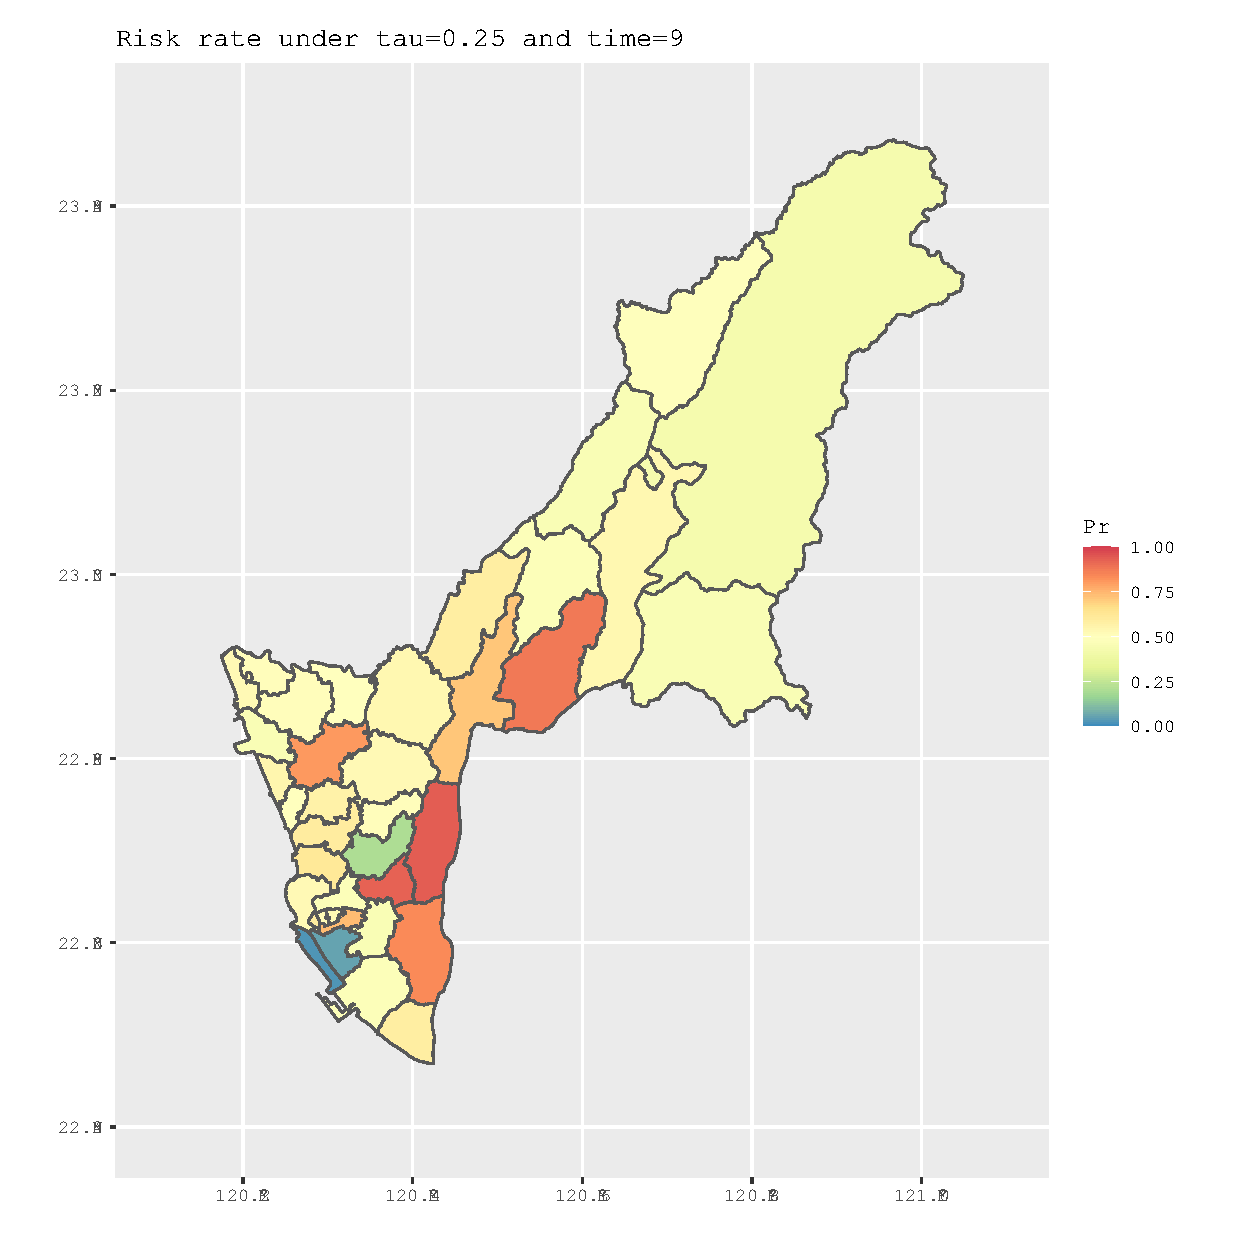
\includegraphics[width=0.22\paperwidth]{Risk_rate_under_tau=0.25_and_time=9.eps}} \\
\subfigure[第十期]{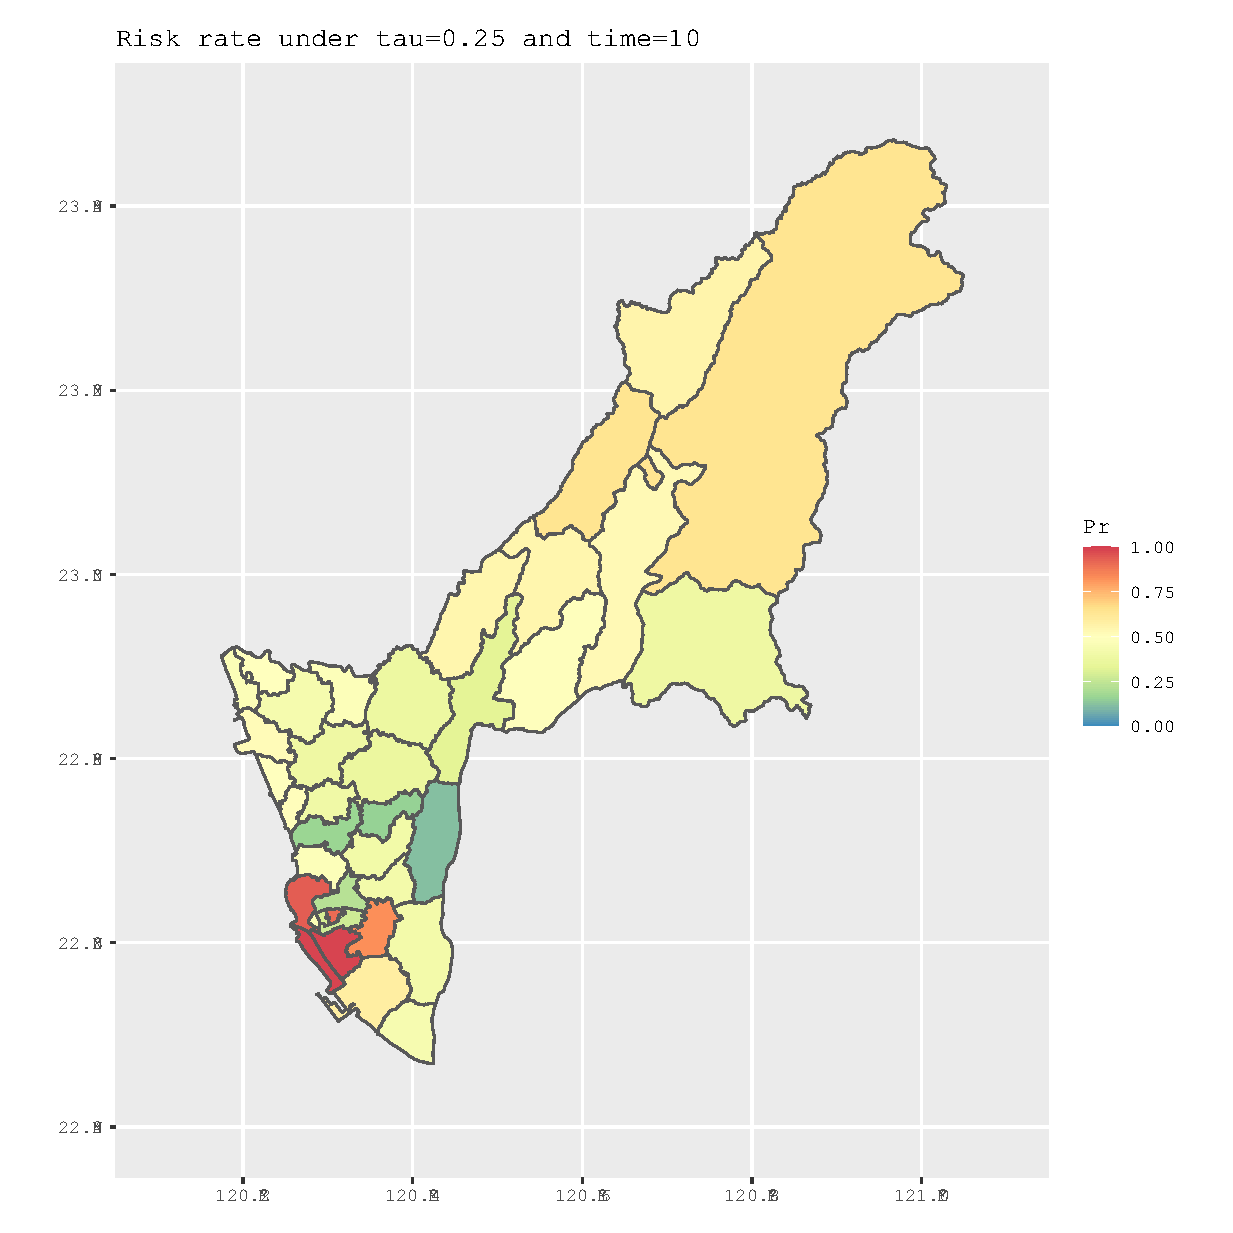
\includegraphics[width=0.22\paperwidth]{Risk_rate_under_tau=0.25_and_time=10.eps}}
\caption{$\tau = 0.25$ 第一期至第十期發生率風險機率圖}
\label{Fig.main7}
\end{figure}

\begin{figure}[htpb]
\centering
\subfigure[第十一期]{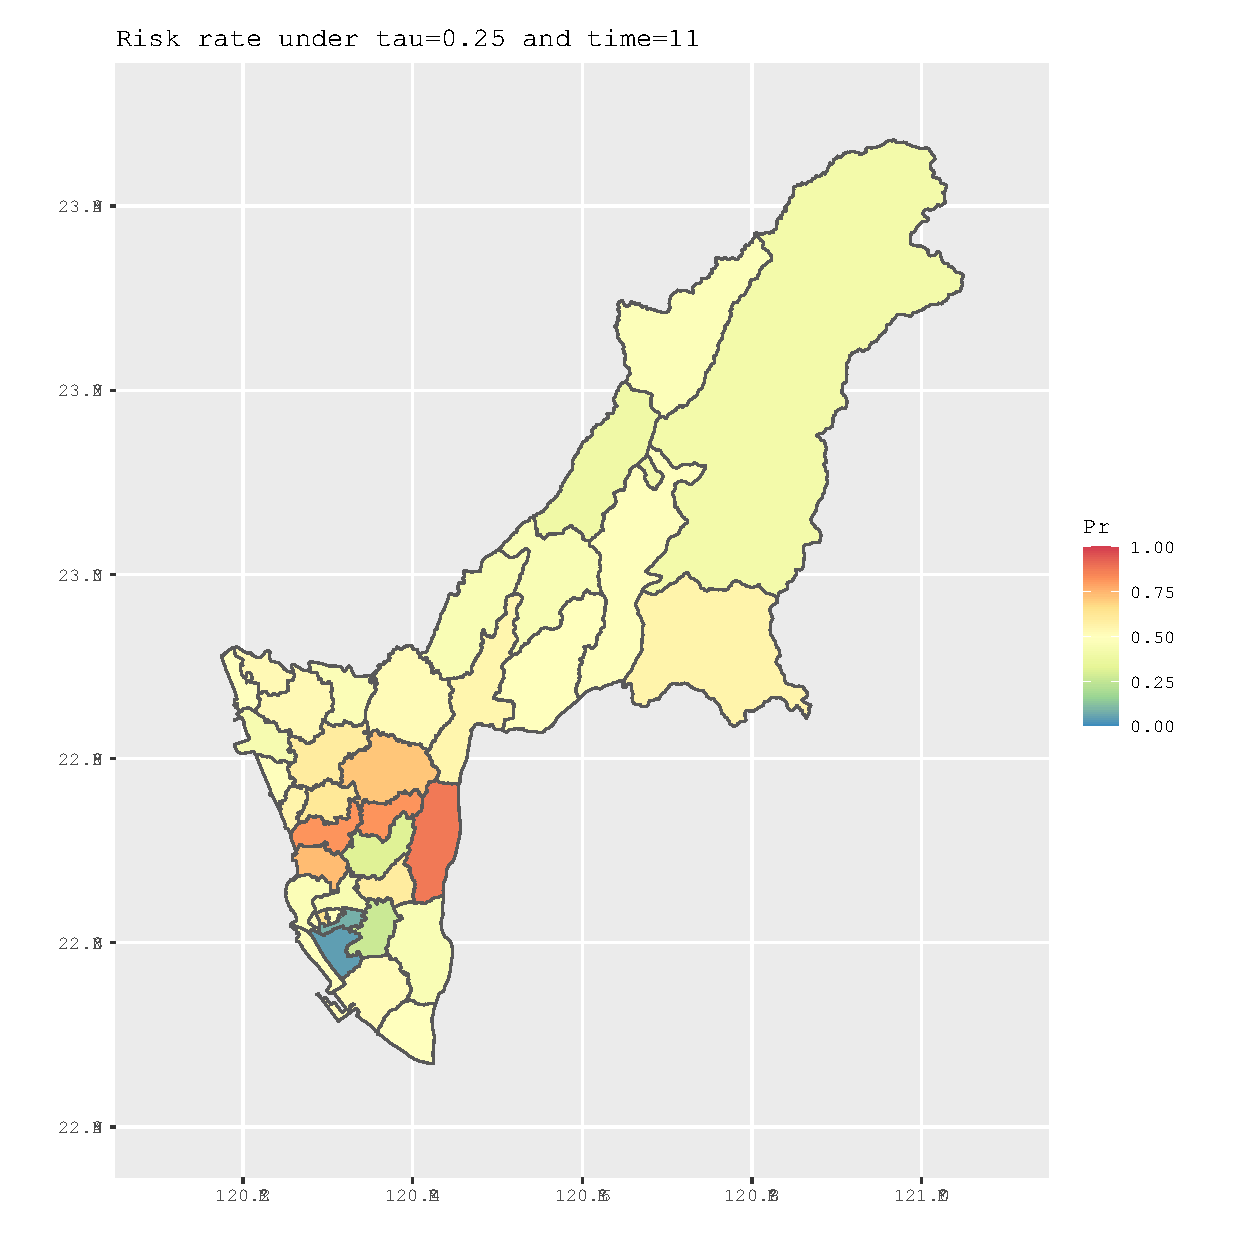
\includegraphics[width=0.22\paperwidth]{Risk_rate_under_tau=0.25_and_time=11.eps}}
\subfigure[第十二期]{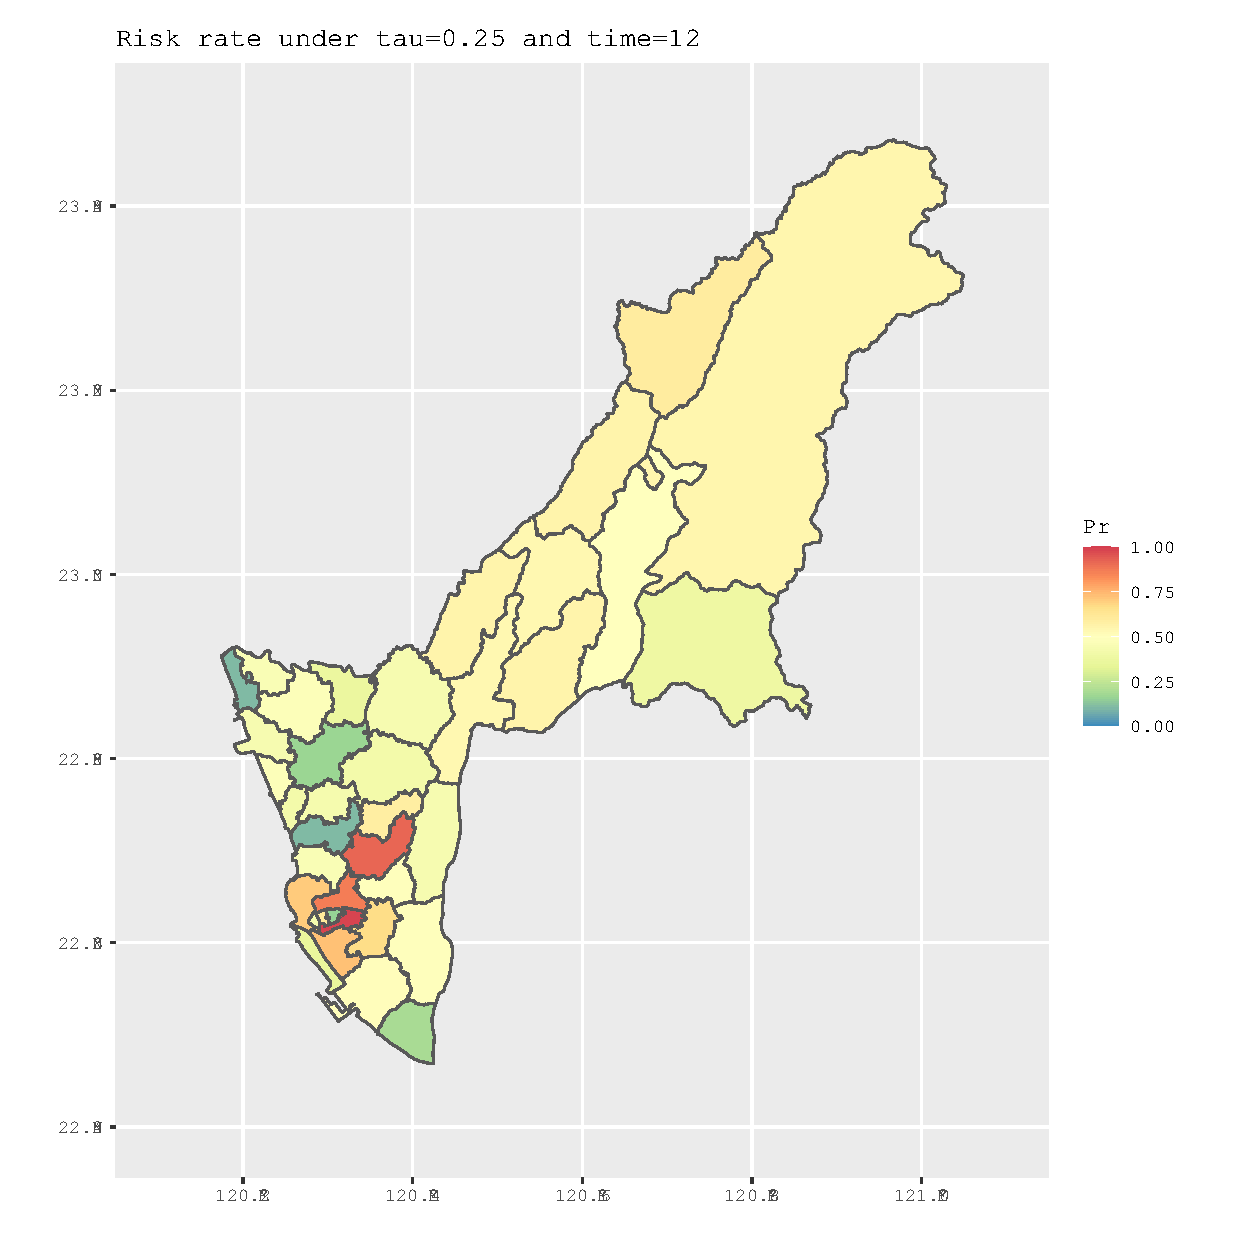
\includegraphics[width=0.22\paperwidth]{Risk_rate_under_tau=0.25_and_time=12.eps}}
\subfigure[第十三期]{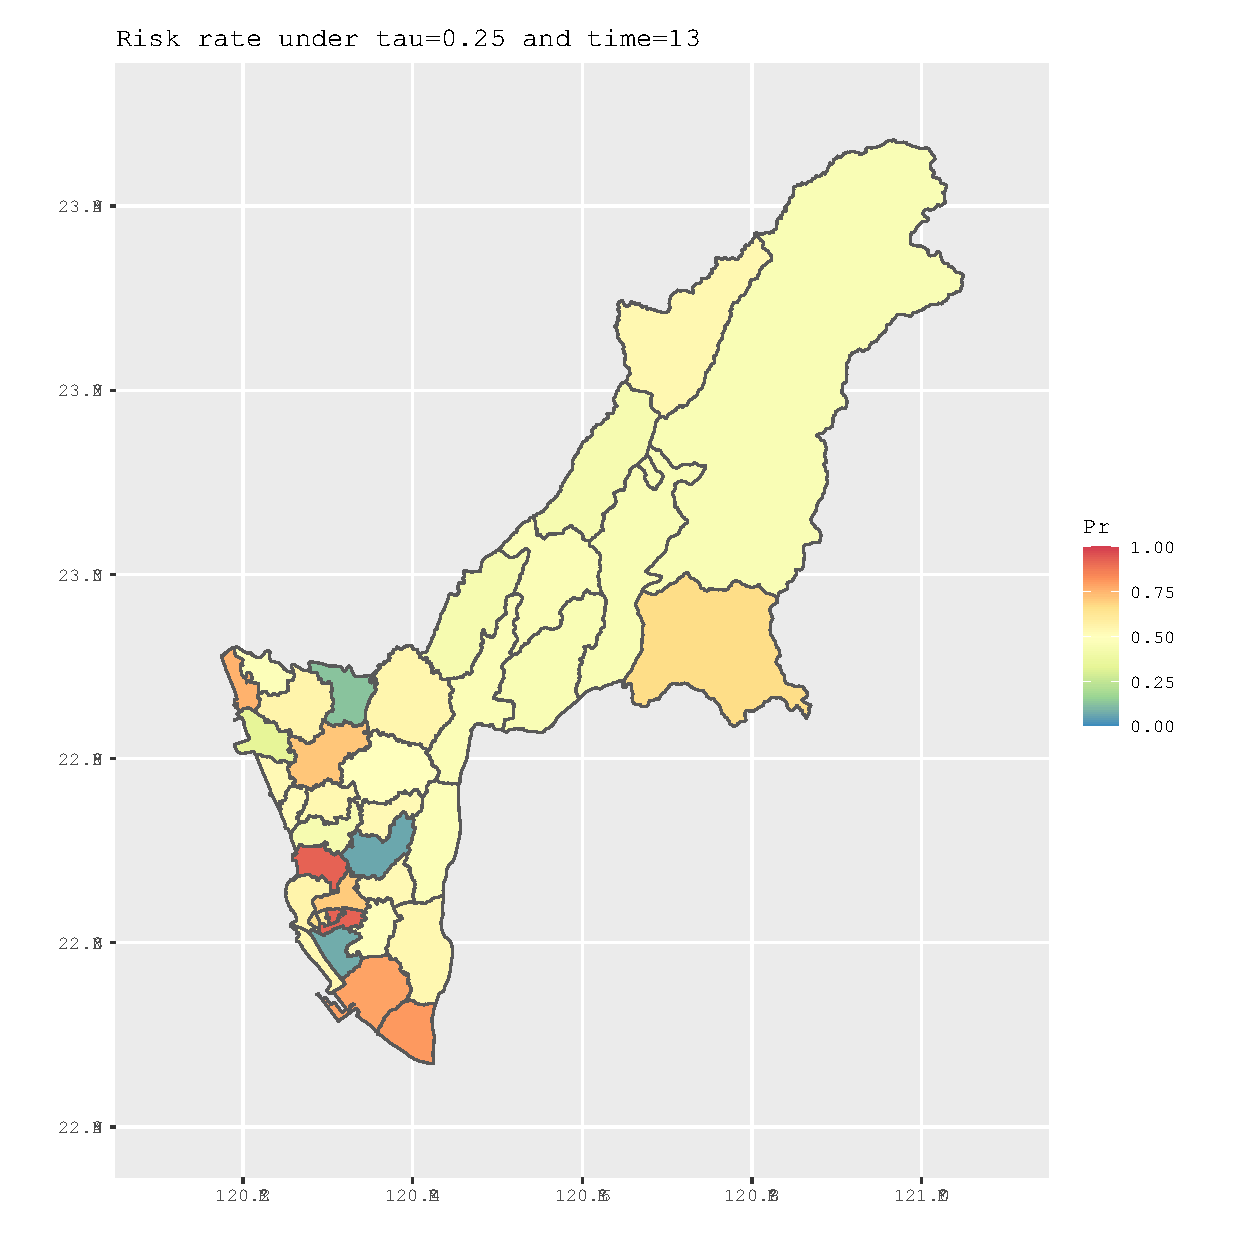
\includegraphics[width=0.22\paperwidth]{Risk_rate_under_tau=0.25_and_time=13.eps}}\\
\subfigure[第十四期]{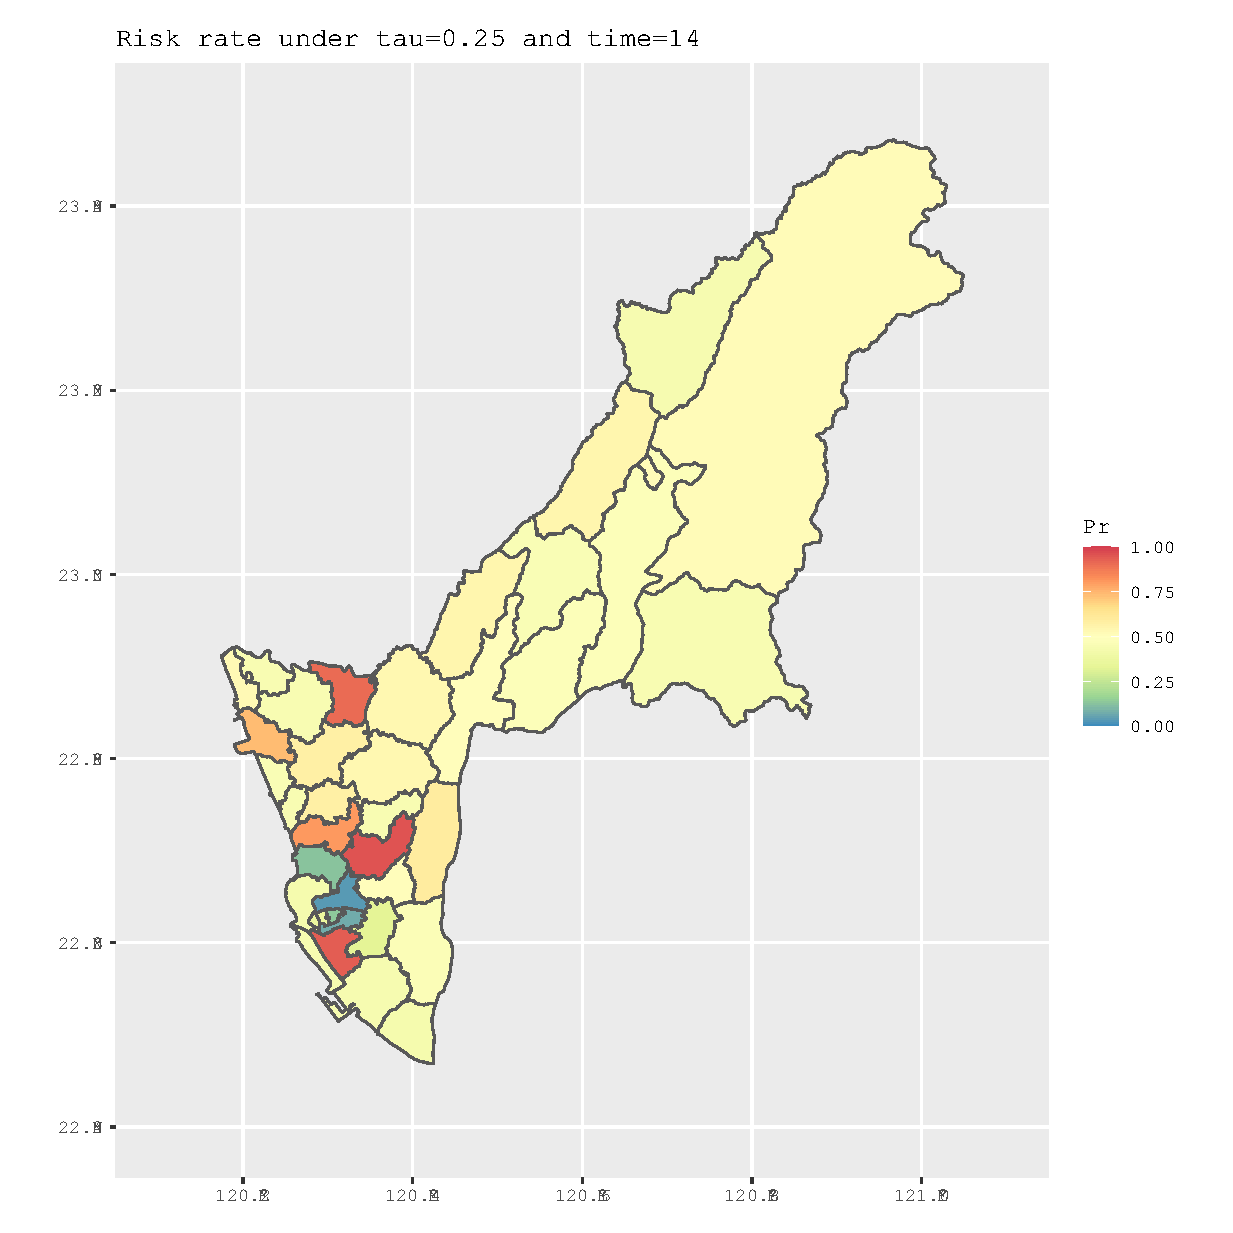
\includegraphics[width=0.22\paperwidth]{Risk_rate_under_tau=0.25_and_time=14.eps}}
\subfigure[第十五期]{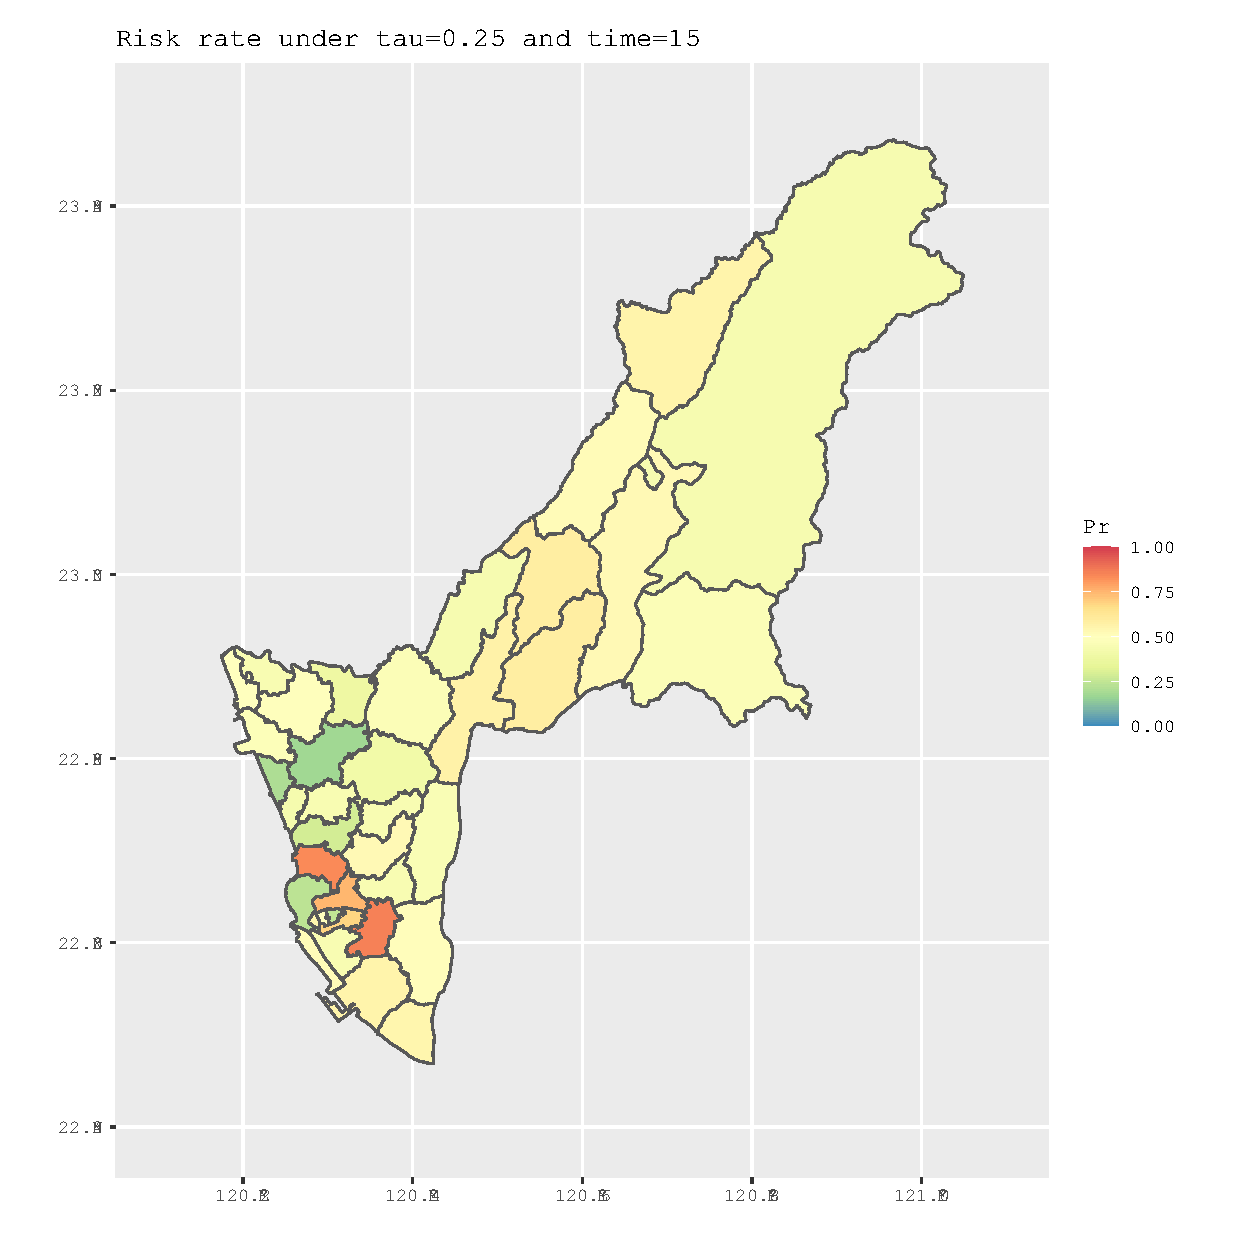
\includegraphics[width=0.22\paperwidth]{Risk_rate_under_tau=0.25_and_time=15.eps}}
\subfigure[第十六期]{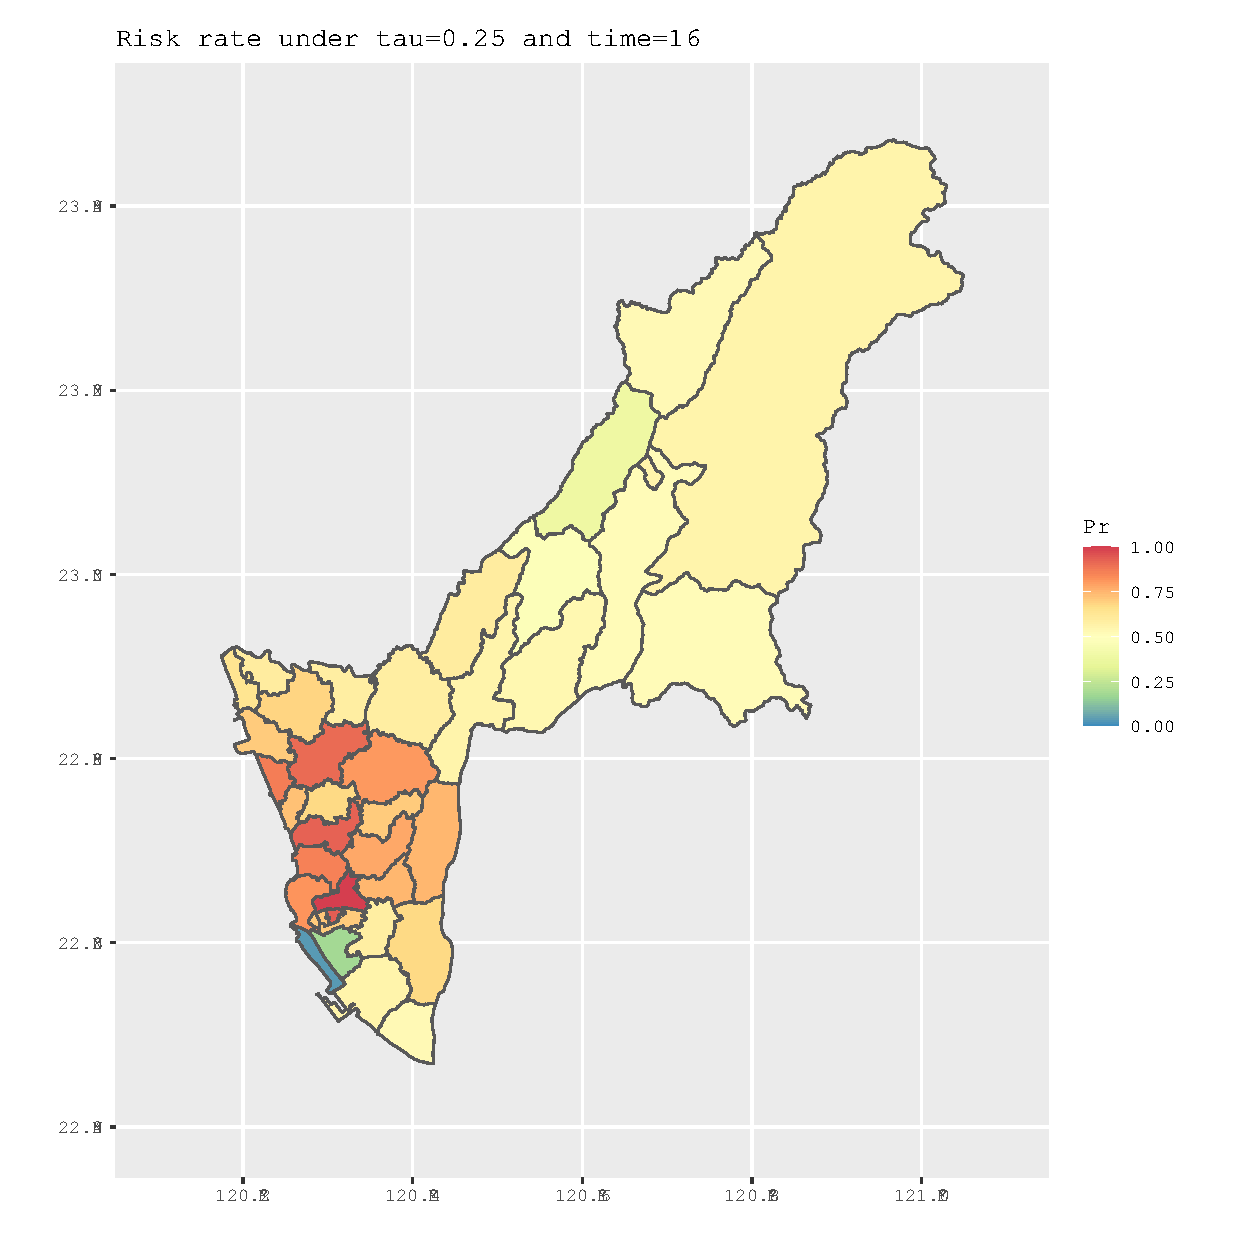
\includegraphics[width=0.22\paperwidth]{Risk_rate_under_tau=0.25_and_time=16.eps}} \\
\subfigure[第十七期]{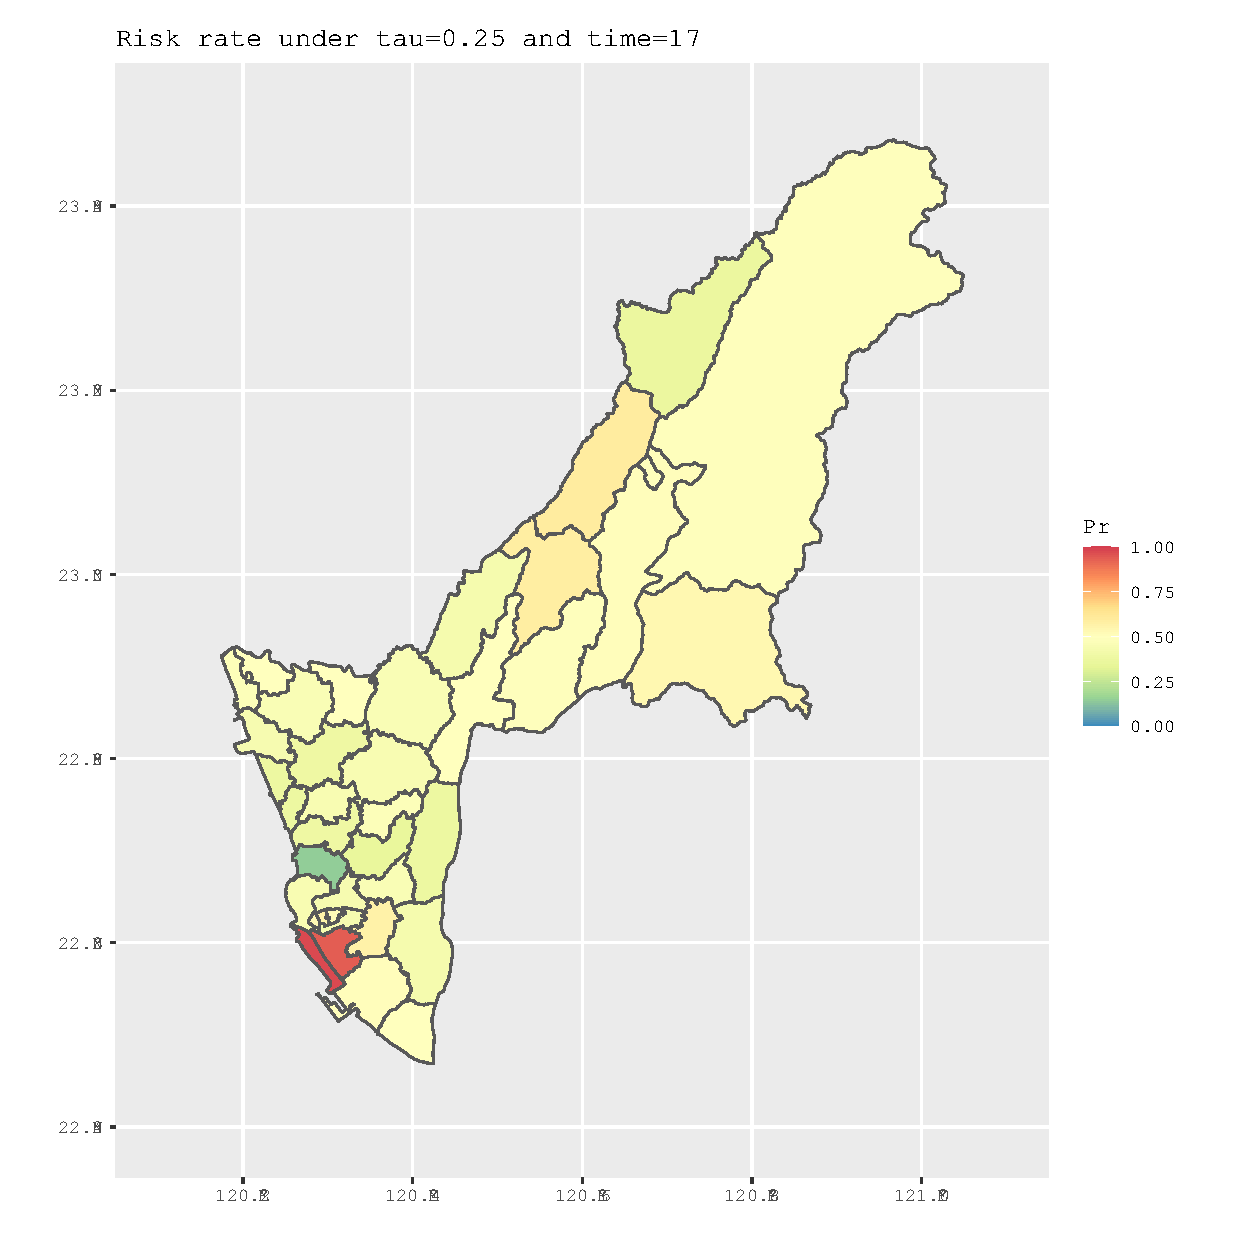
\includegraphics[width=0.22\paperwidth]{Risk_rate_under_tau=0.25_and_time=17.eps}}
\subfigure[第十八期]{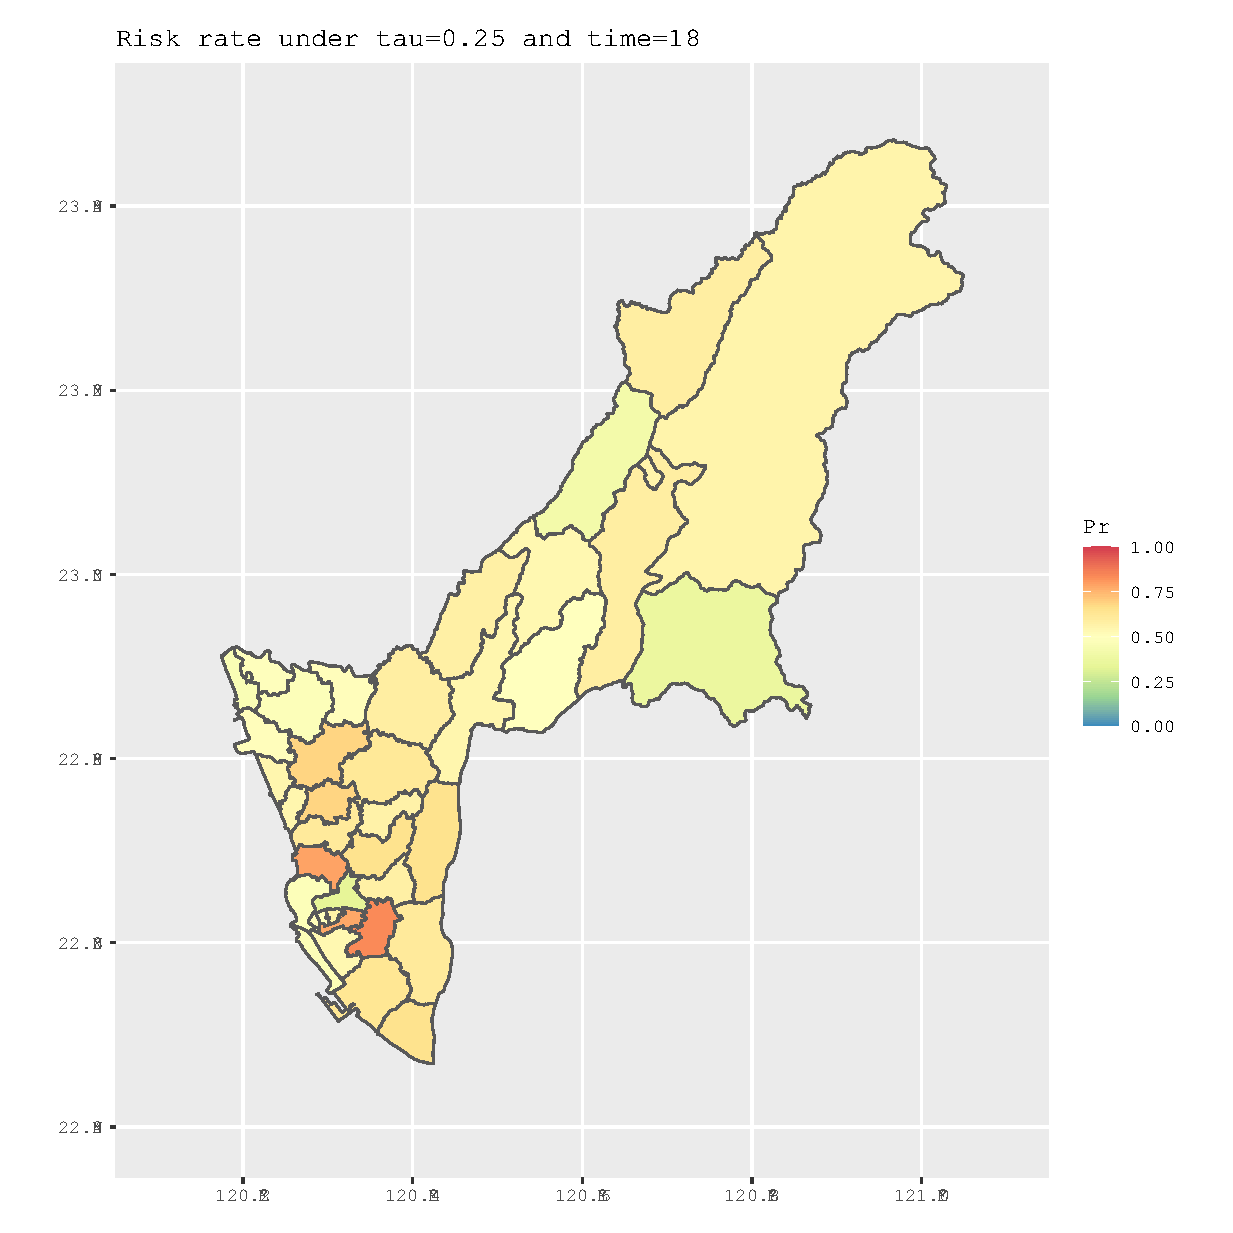
\includegraphics[width=0.22\paperwidth]{Risk_rate_under_tau=0.25_and_time=18.eps}}
\subfigure[第十九期]{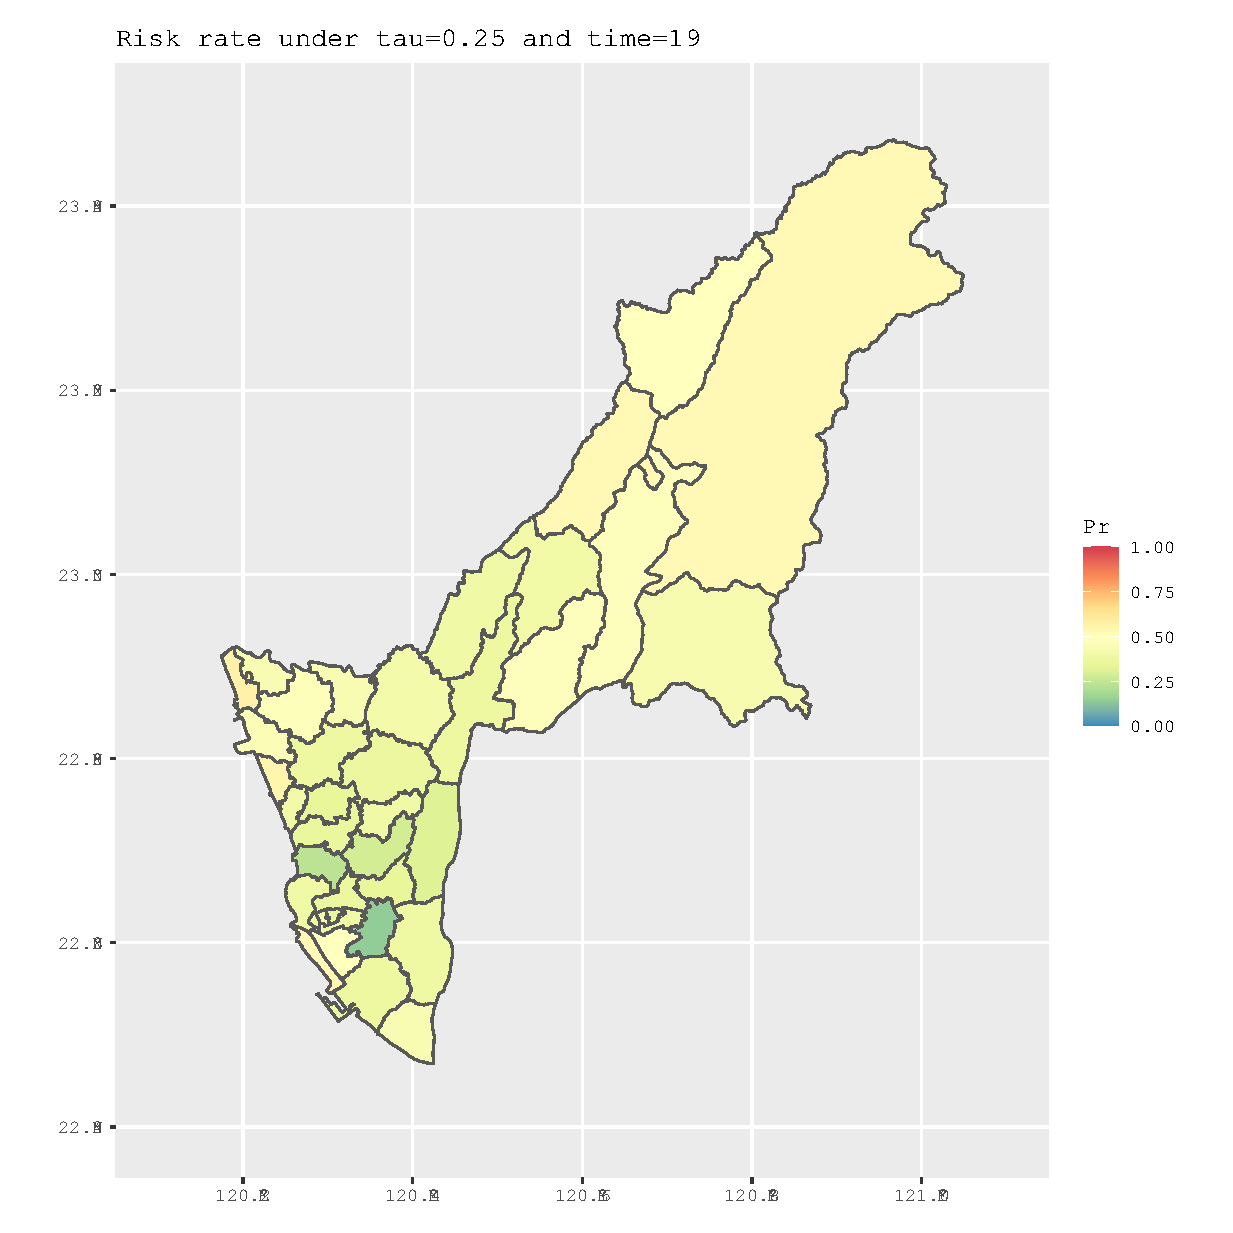
\includegraphics[width=0.22\paperwidth]{Risk_rate_under_tau=0.25_and_time=19.eps}}
\caption{$\tau = 0.25$ 第十一期至第十九期發生率風險機率圖}
\label{Fig.main8}
\end{figure}

\begin{figure}[htpb]
\centering
\subfigure[第一期]{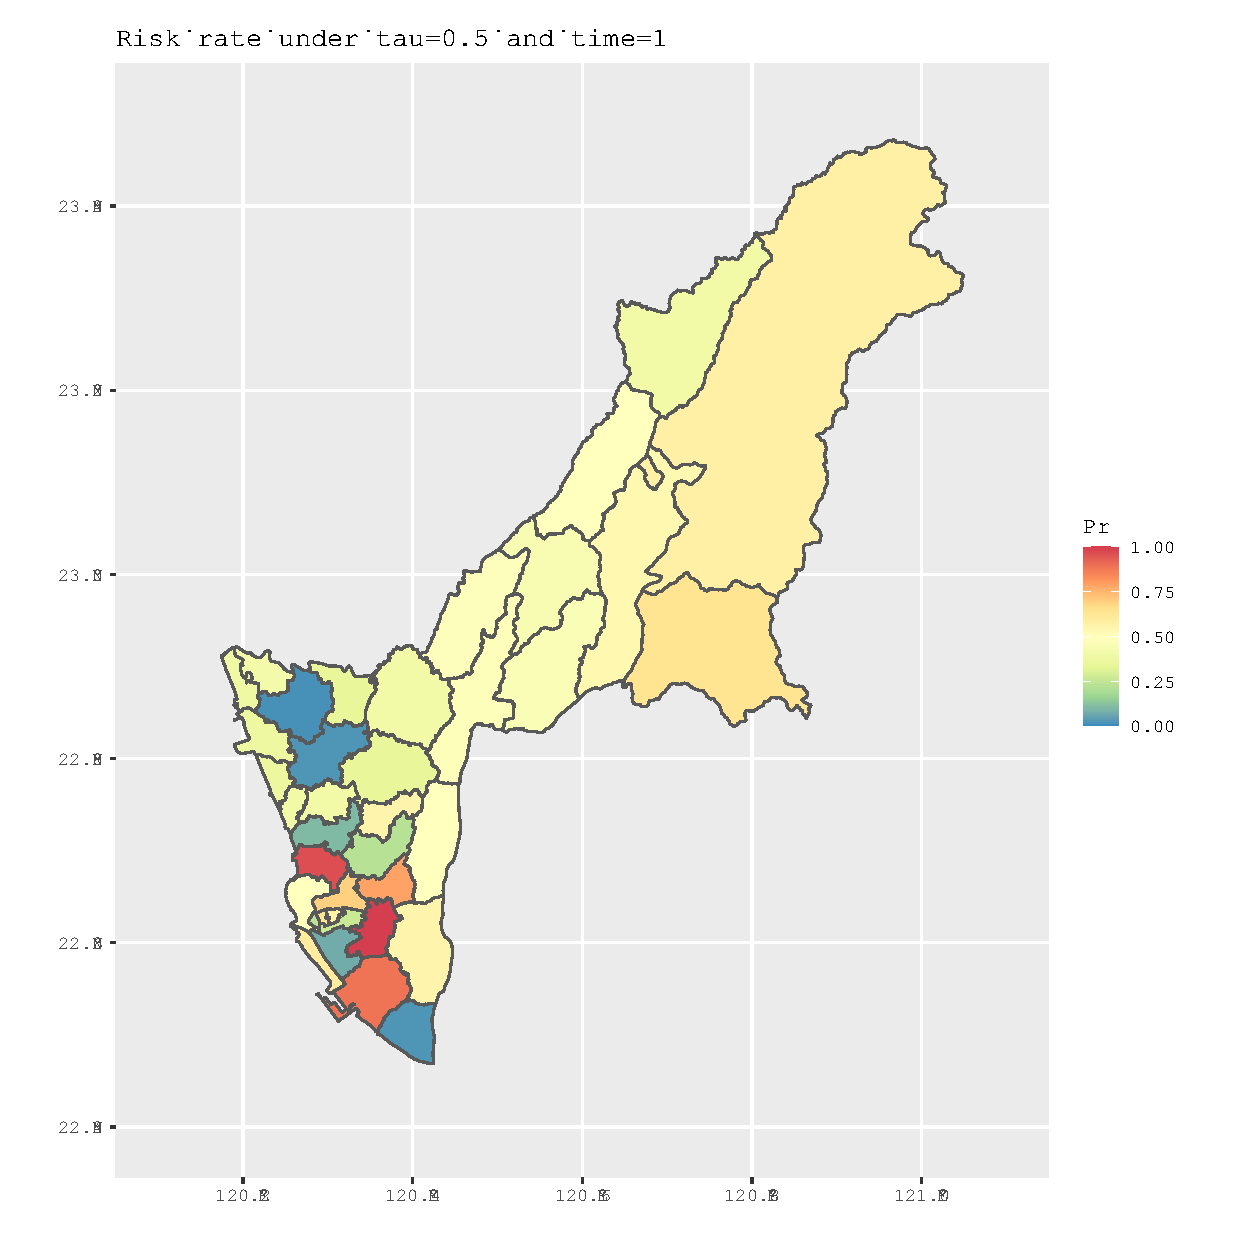
\includegraphics[width=0.22\paperwidth]{Risk_rate_under_tau=0.5_and_time=1.eps}}
\subfigure[第二期]{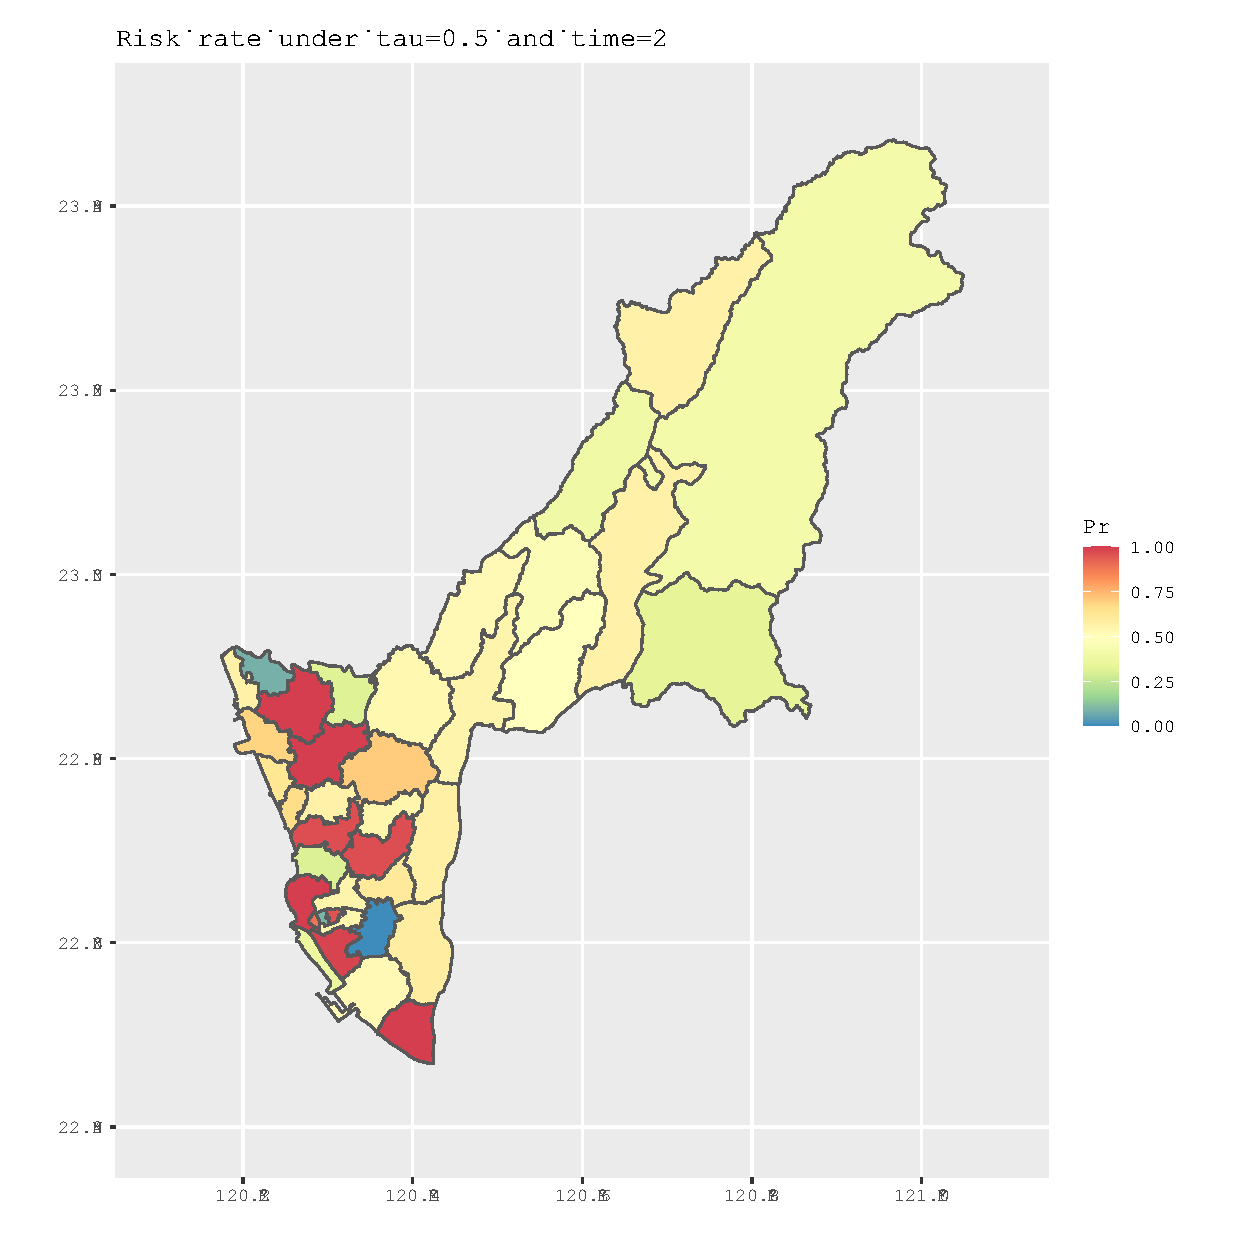
\includegraphics[width=0.22\paperwidth]{Risk_rate_under_tau=0.5_and_time=2.eps}}
\subfigure[第三期]{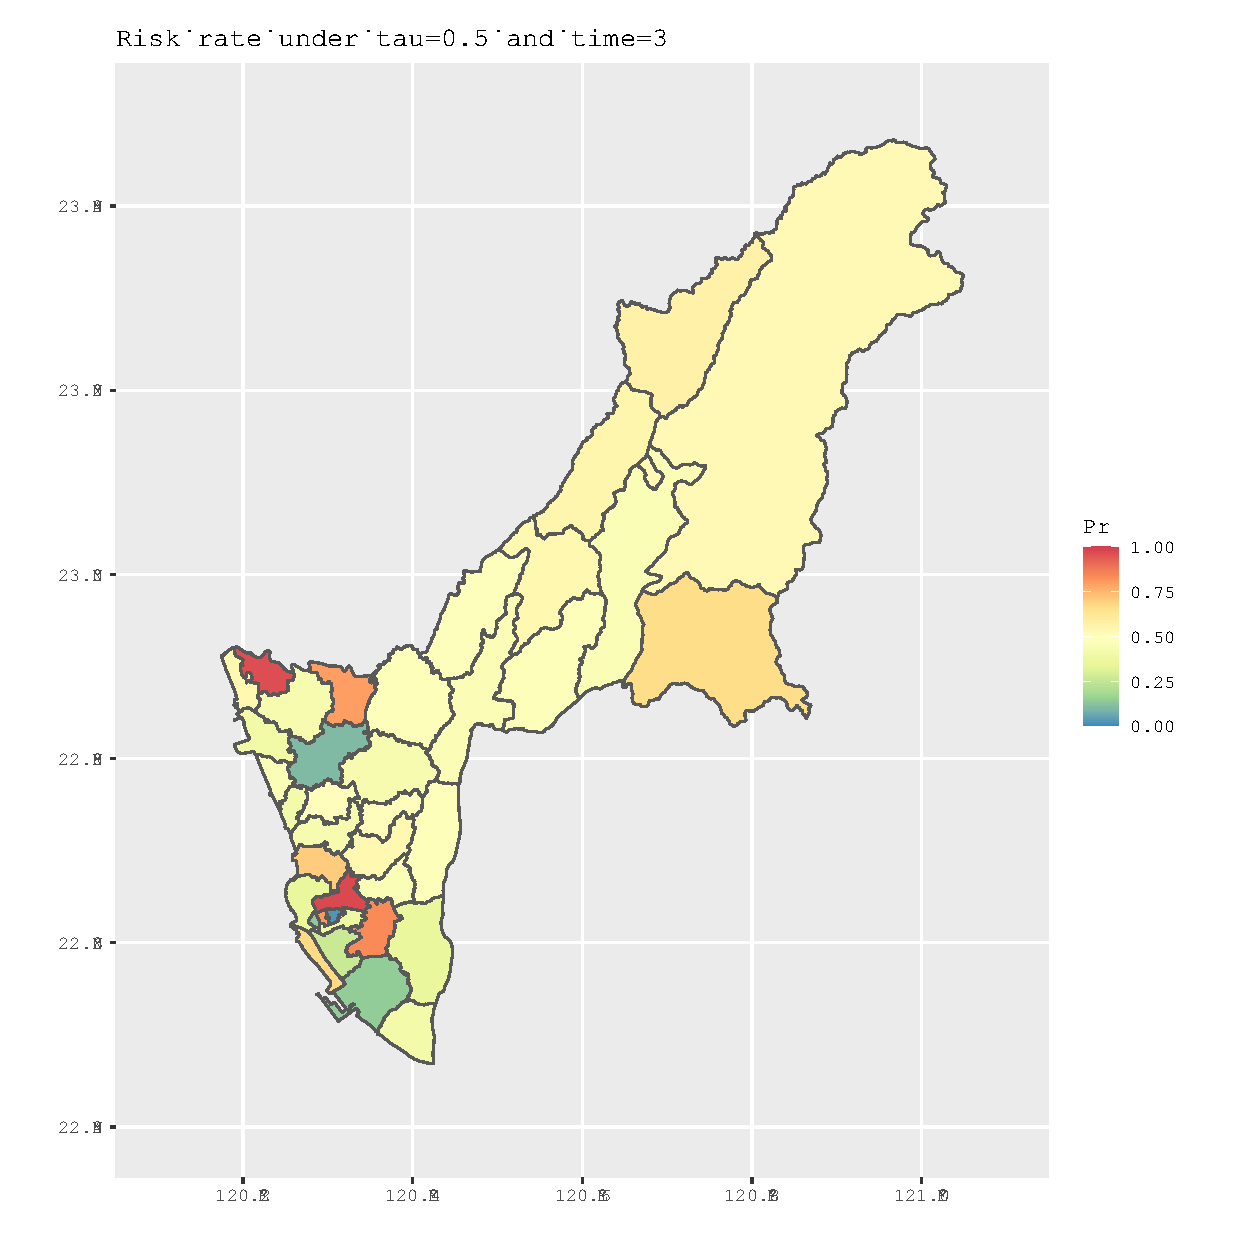
\includegraphics[width=0.22\paperwidth]{Risk_rate_under_tau=0.5_and_time=3.eps}} \\
\subfigure[第四期]{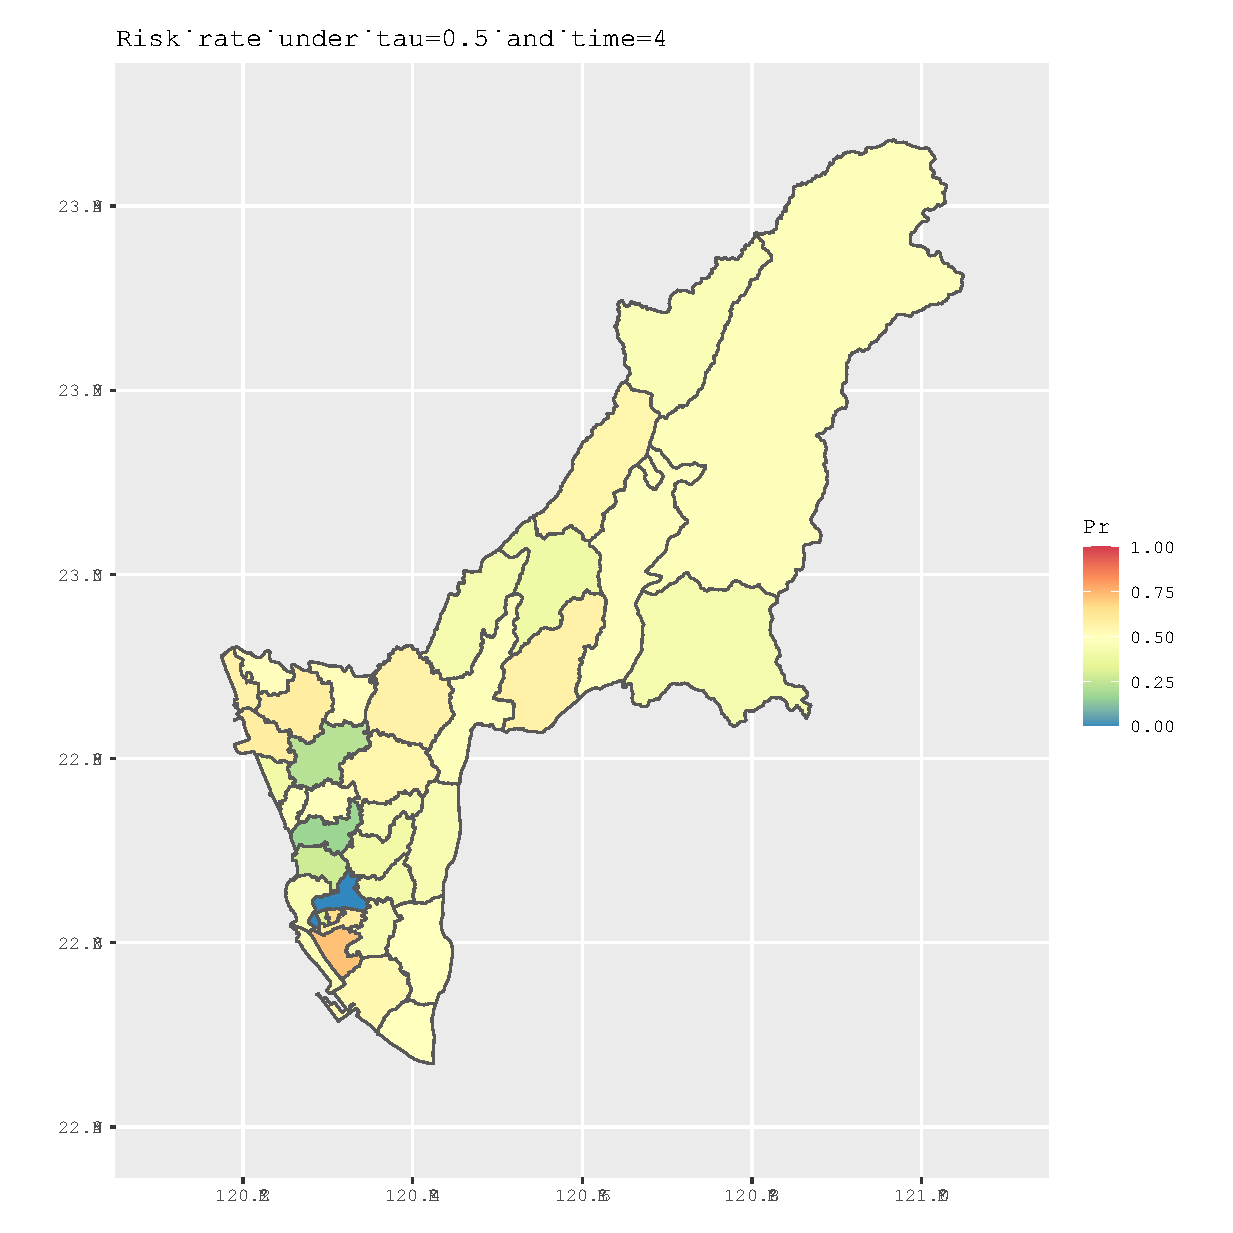
\includegraphics[width=0.22\paperwidth]{Risk_rate_under_tau=0.5_and_time=4.eps}}
\subfigure[第五期]{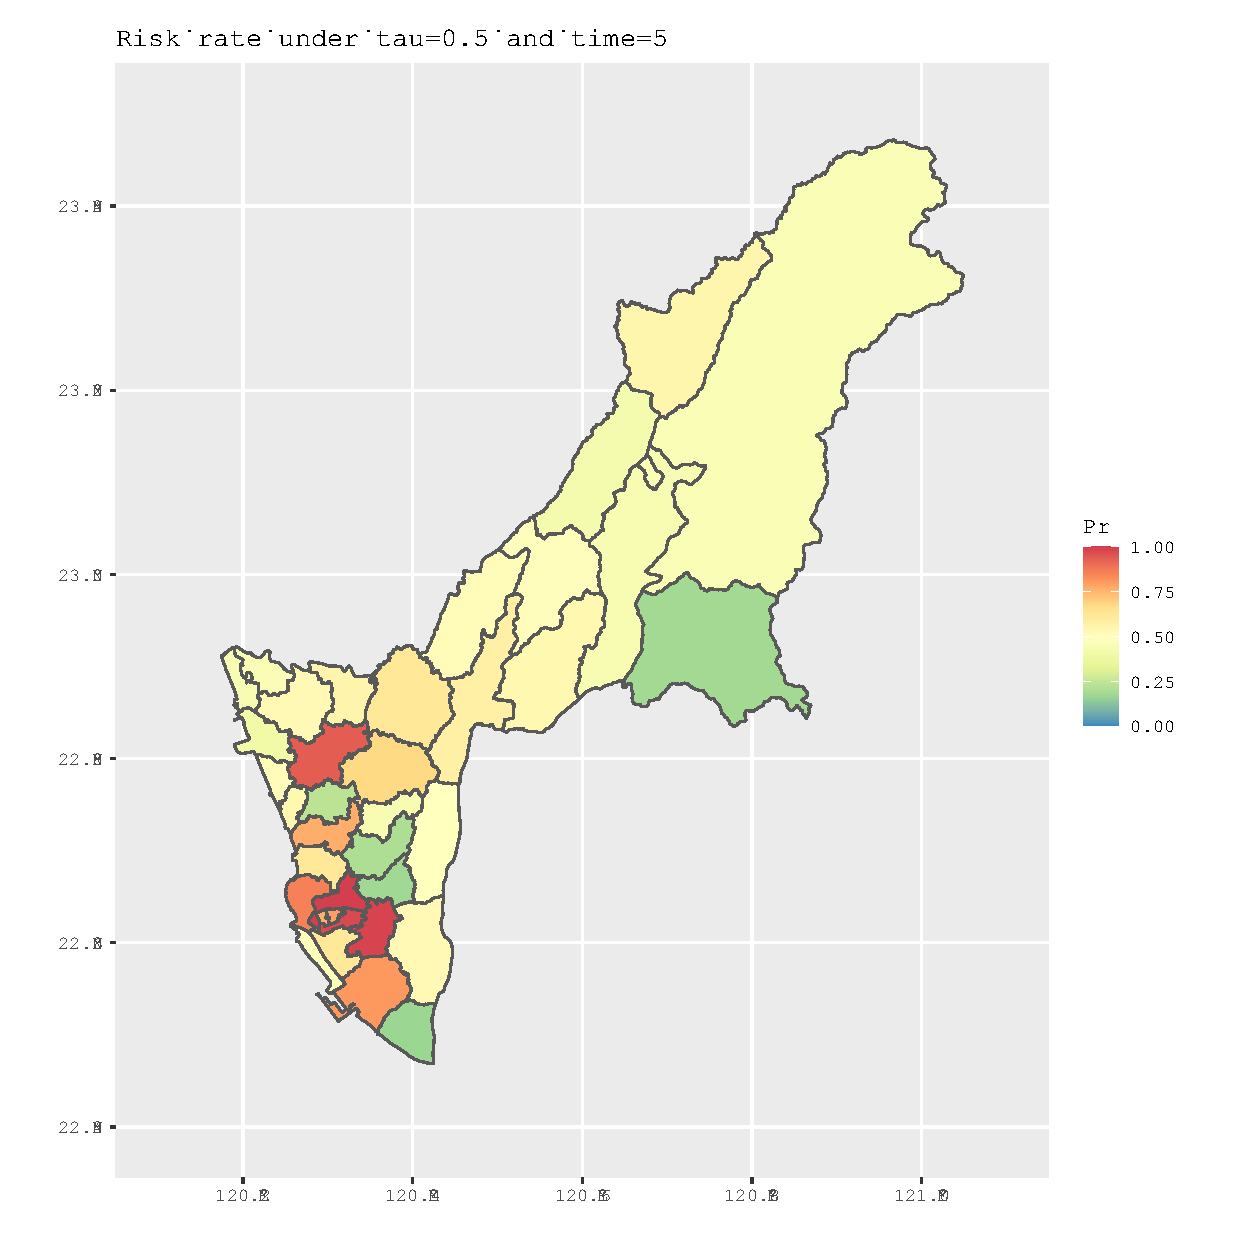
\includegraphics[width=0.22\paperwidth]{Risk_rate_under_tau=0.5_and_time=5.eps}}
\subfigure[第六期]{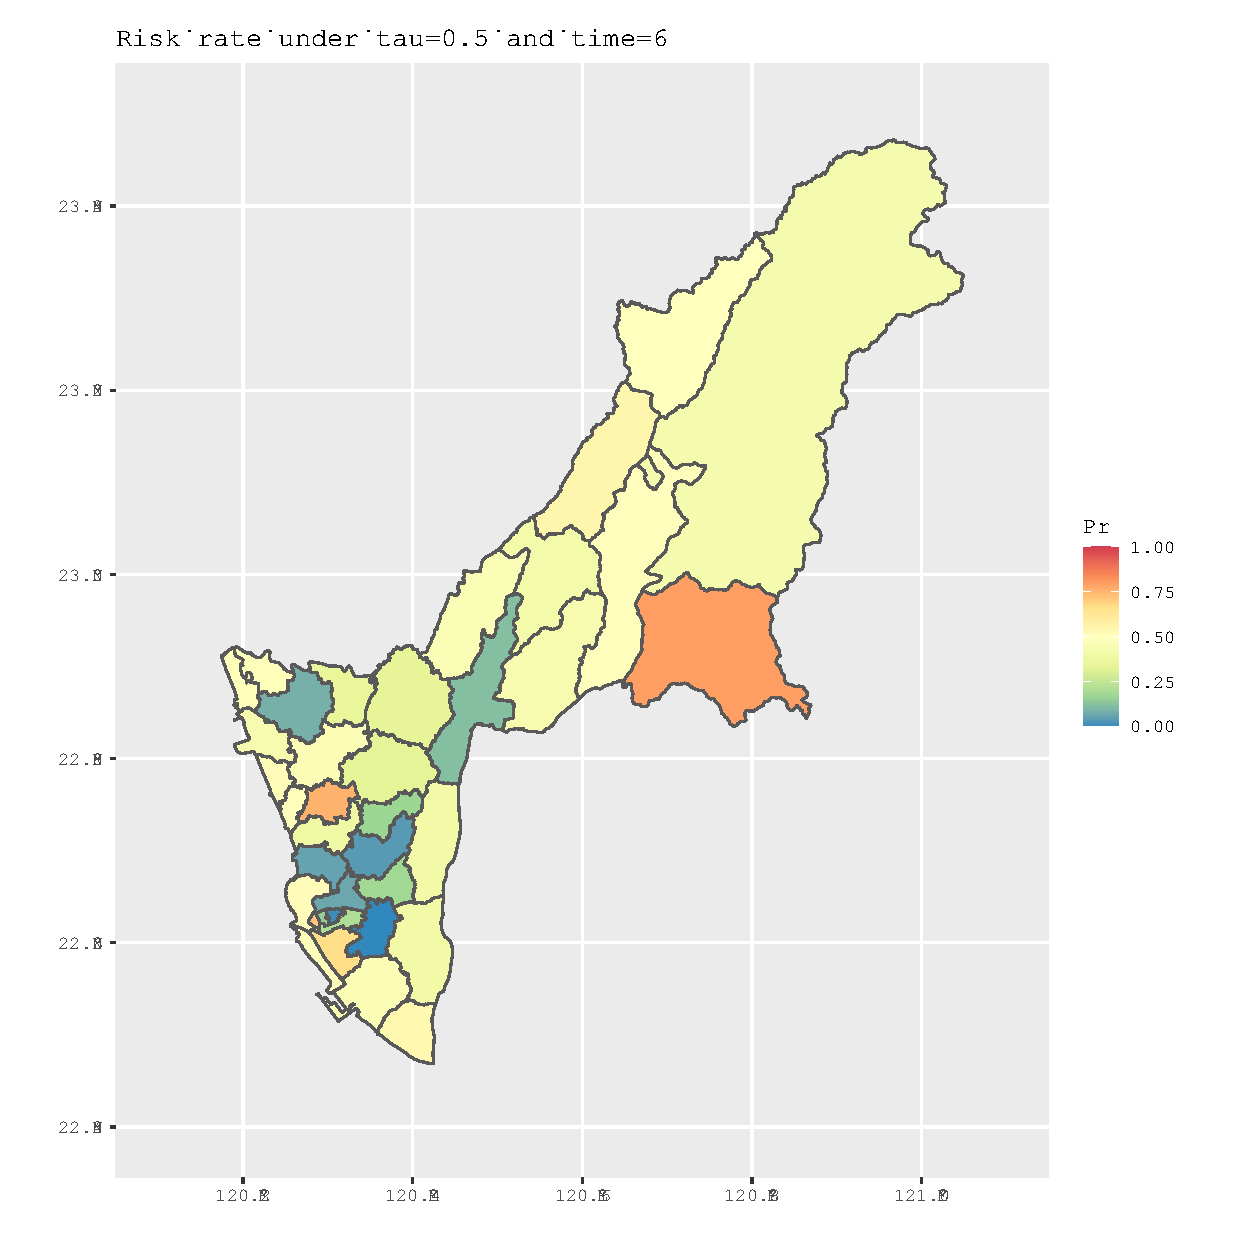
\includegraphics[width=0.22\paperwidth]{Risk_rate_under_tau=0.5_and_time=6.eps}} \\
\subfigure[第七期]{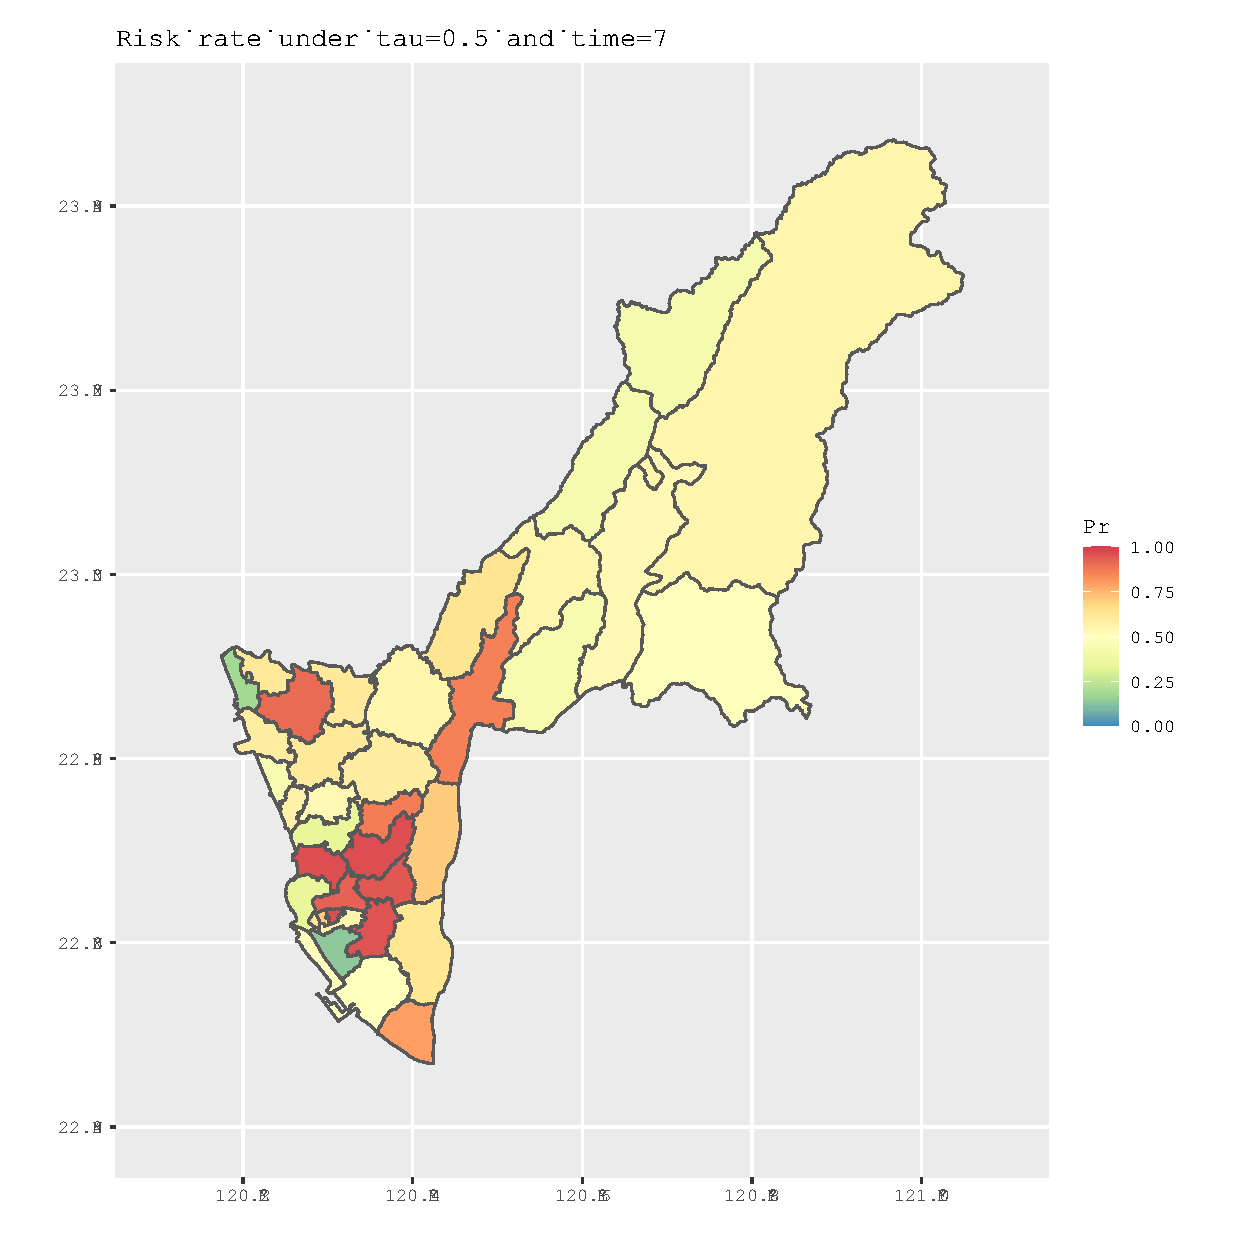
\includegraphics[width=0.22\paperwidth]{Risk_rate_under_tau=0.5_and_time=7.eps}}
\subfigure[第八期]{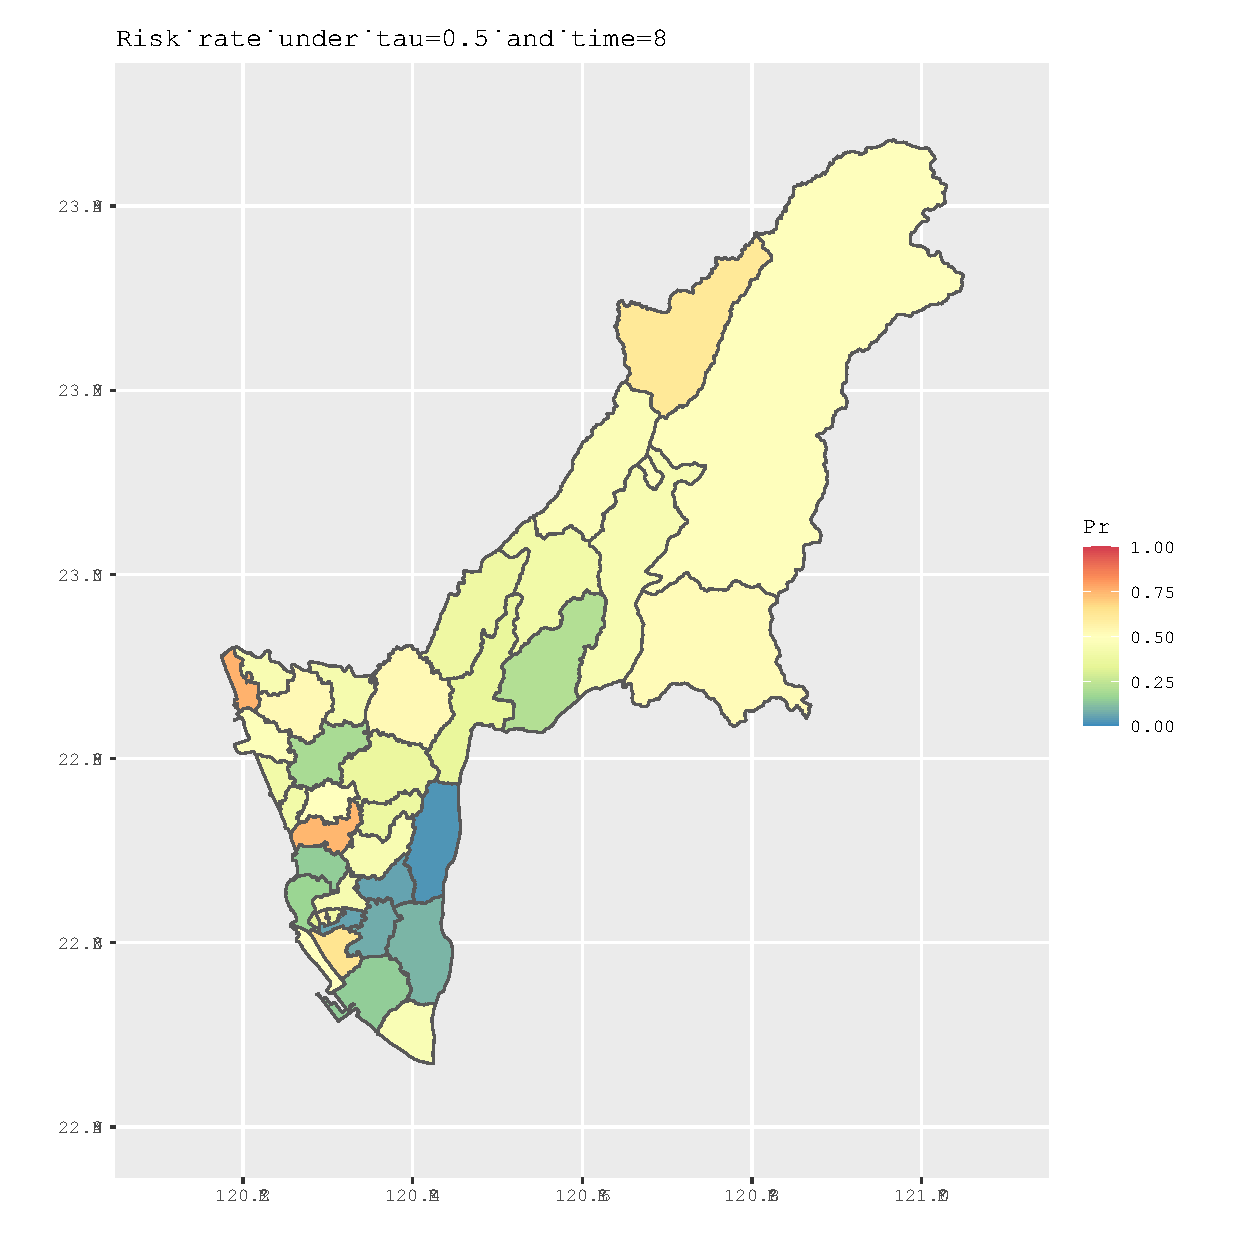
\includegraphics[width=0.22\paperwidth]{Risk_rate_under_tau=0.5_and_time=8.eps}}
\subfigure[第九期]{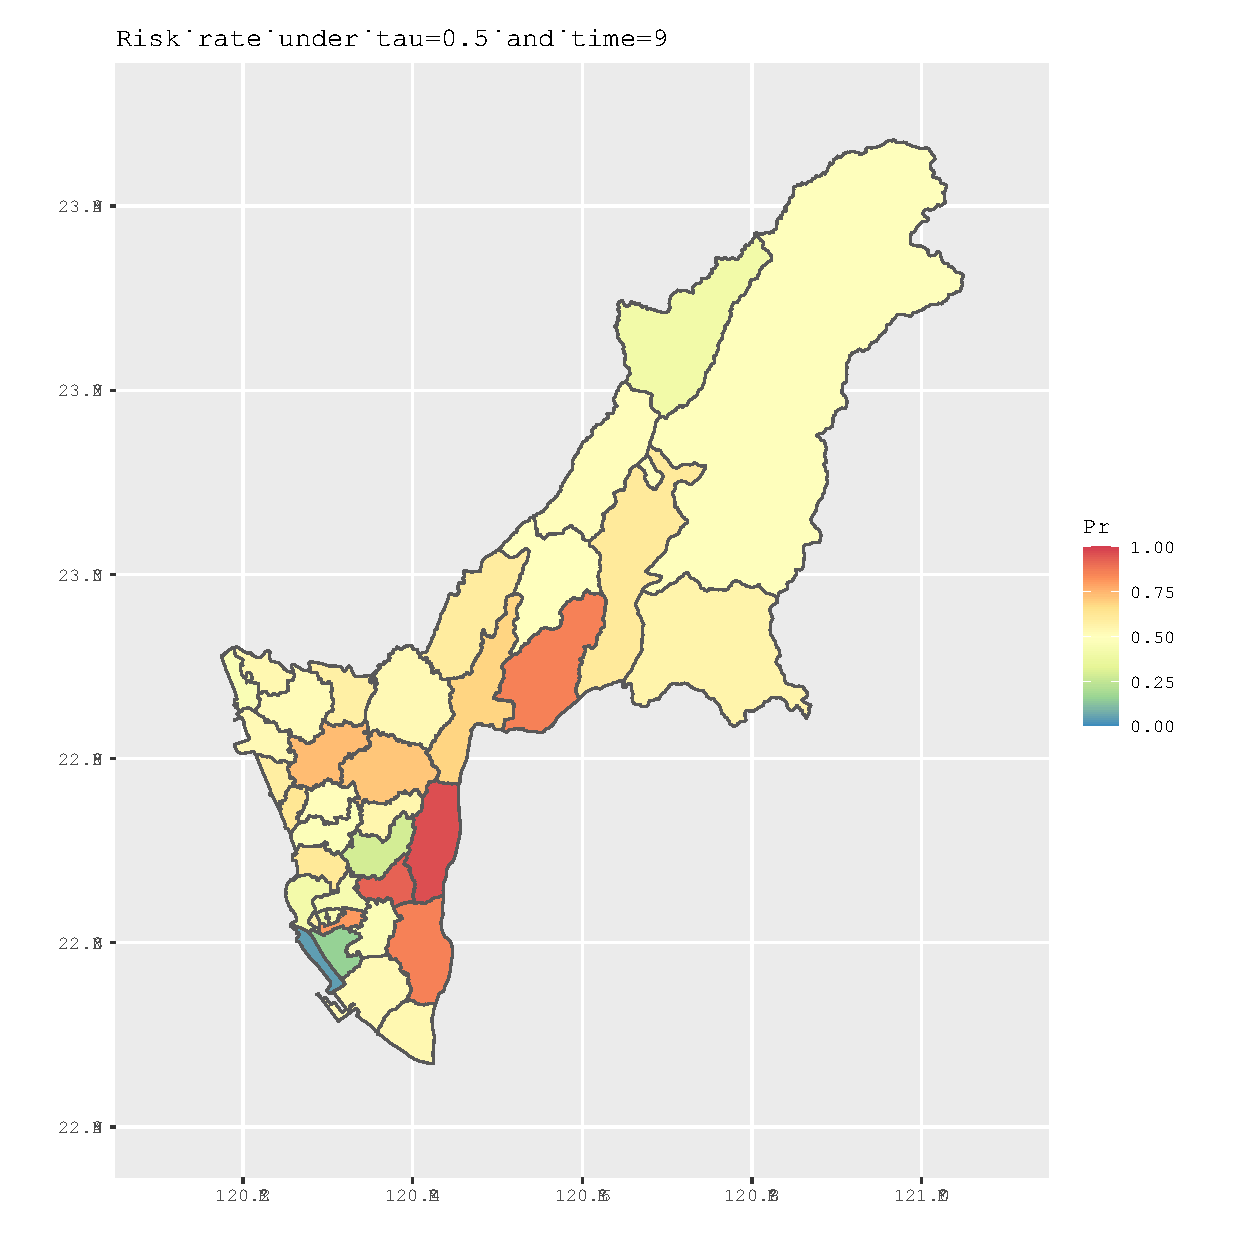
\includegraphics[width=0.22\paperwidth]{Risk_rate_under_tau=0.5_and_time=9.eps}} \\
\subfigure[第十期]{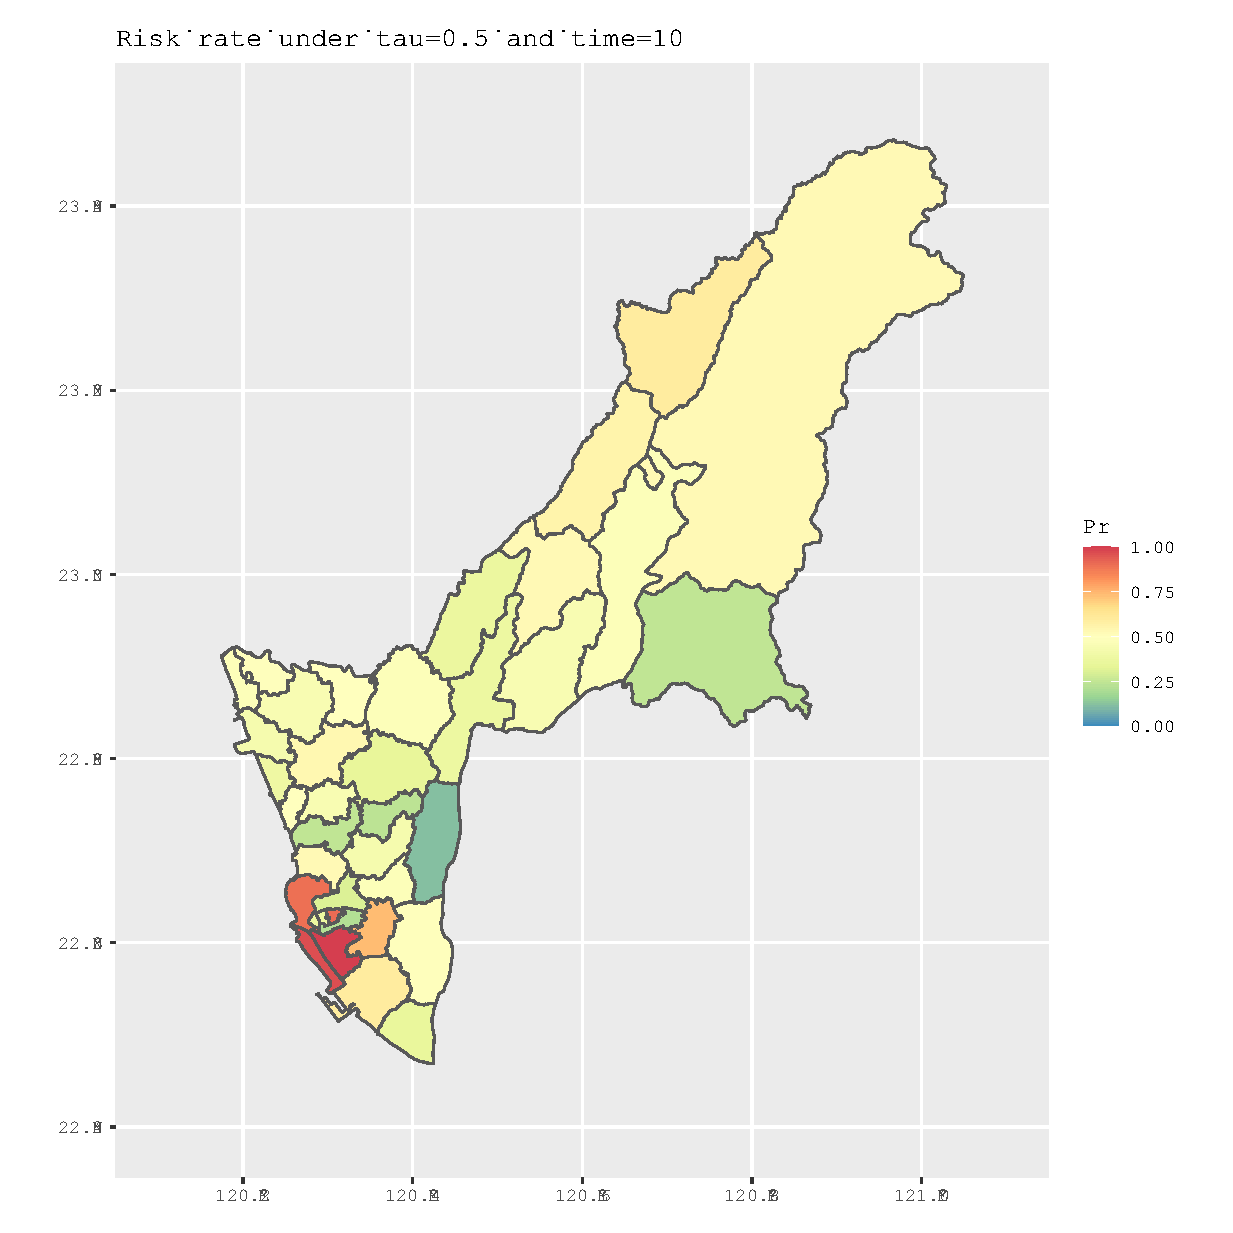
\includegraphics[width=0.22\paperwidth]{Risk_rate_under_tau=0.5_and_time=10.eps}}
\caption{$\tau = 0.5$ 第一期至第十期發生率風險機率圖}
\label{Fig.main9}
\end{figure}

\begin{figure}[htpb]
\centering
\subfigure[第十一期]{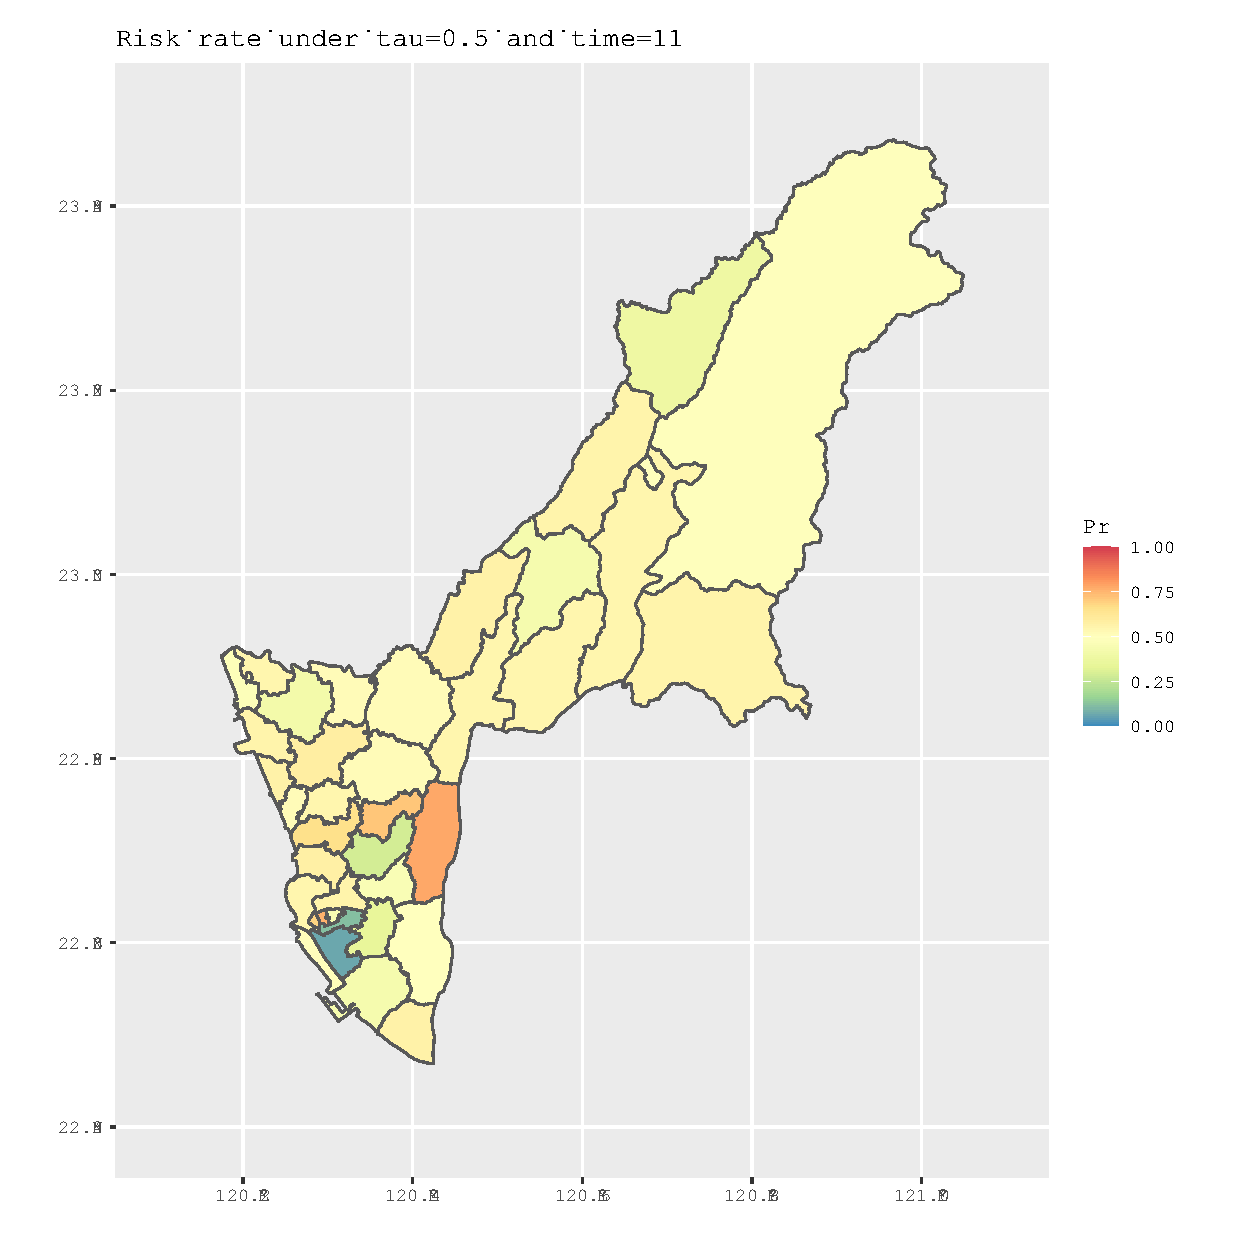
\includegraphics[width=0.22\paperwidth]{Risk_rate_under_tau=0.5_and_time=11.eps}}
\subfigure[第十二期]{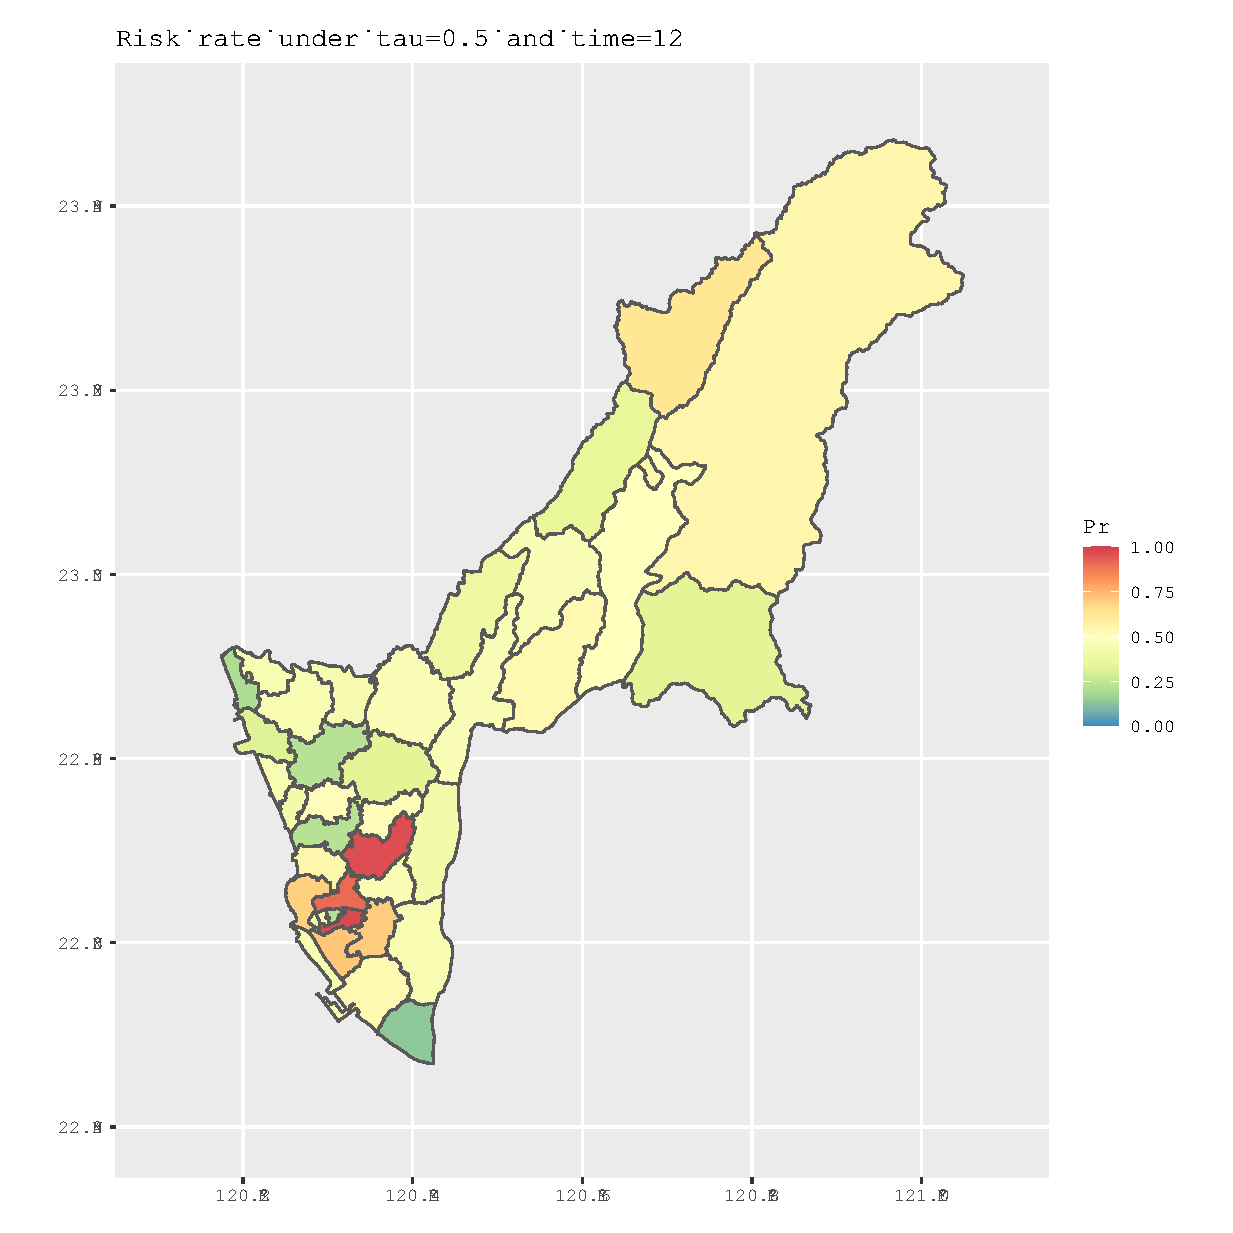
\includegraphics[width=0.22\paperwidth]{Risk_rate_under_tau=0.5_and_time=12.eps}}
\subfigure[第十三期]{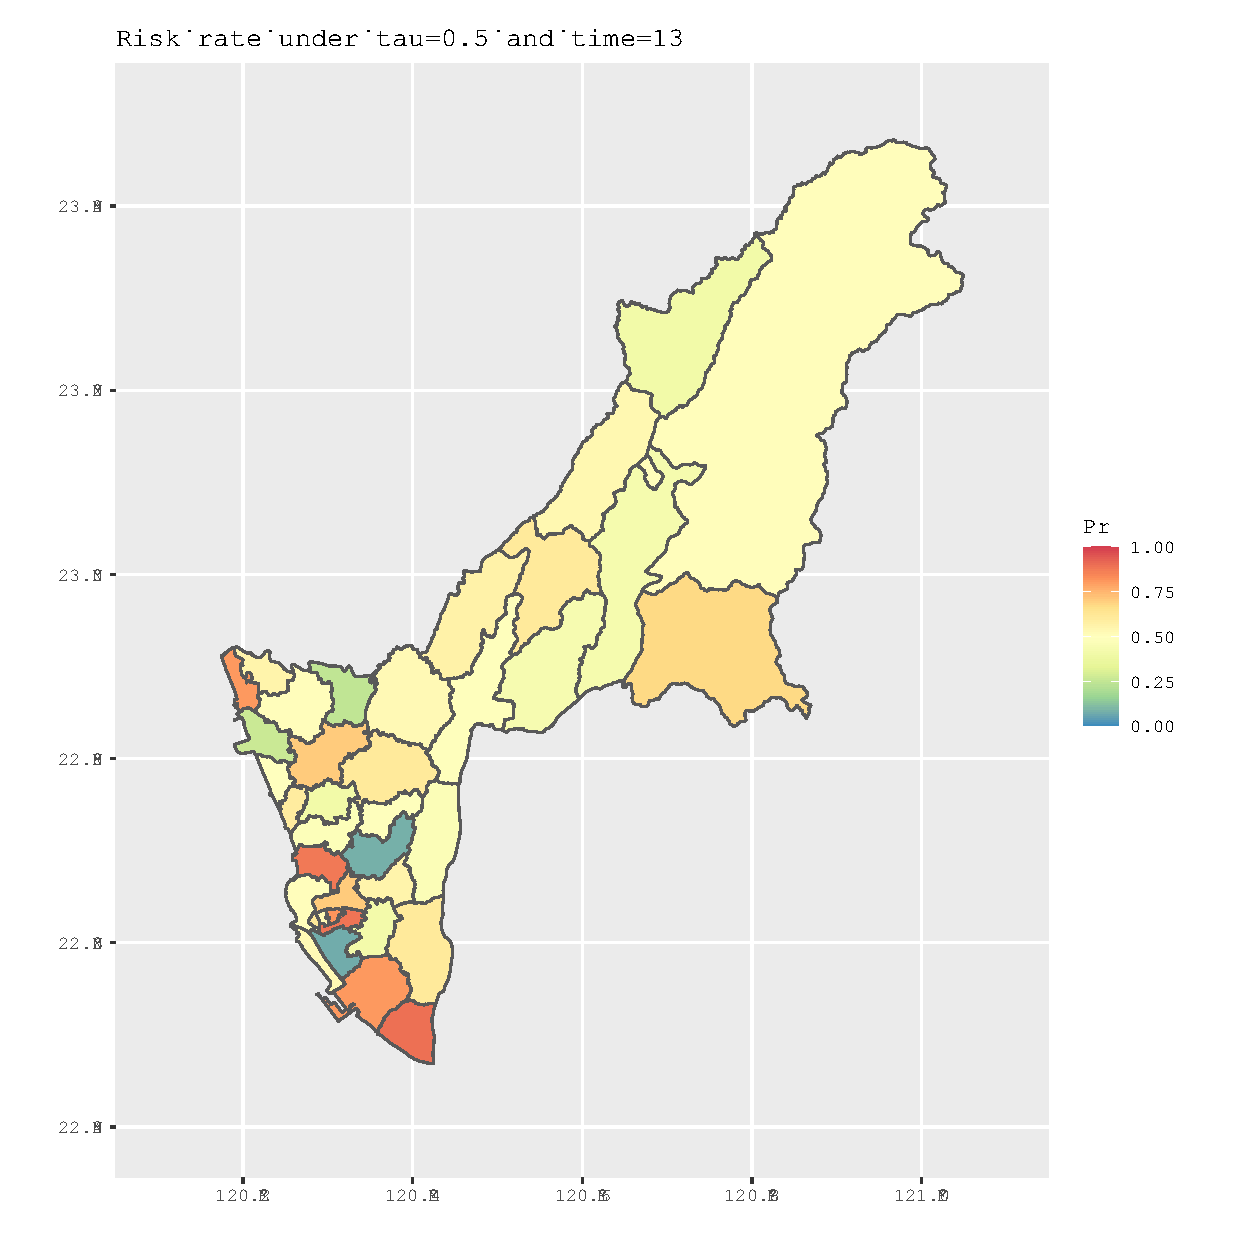
\includegraphics[width=0.22\paperwidth]{Risk_rate_under_tau=0.5_and_time=13.eps}}\\
\subfigure[第十四期]{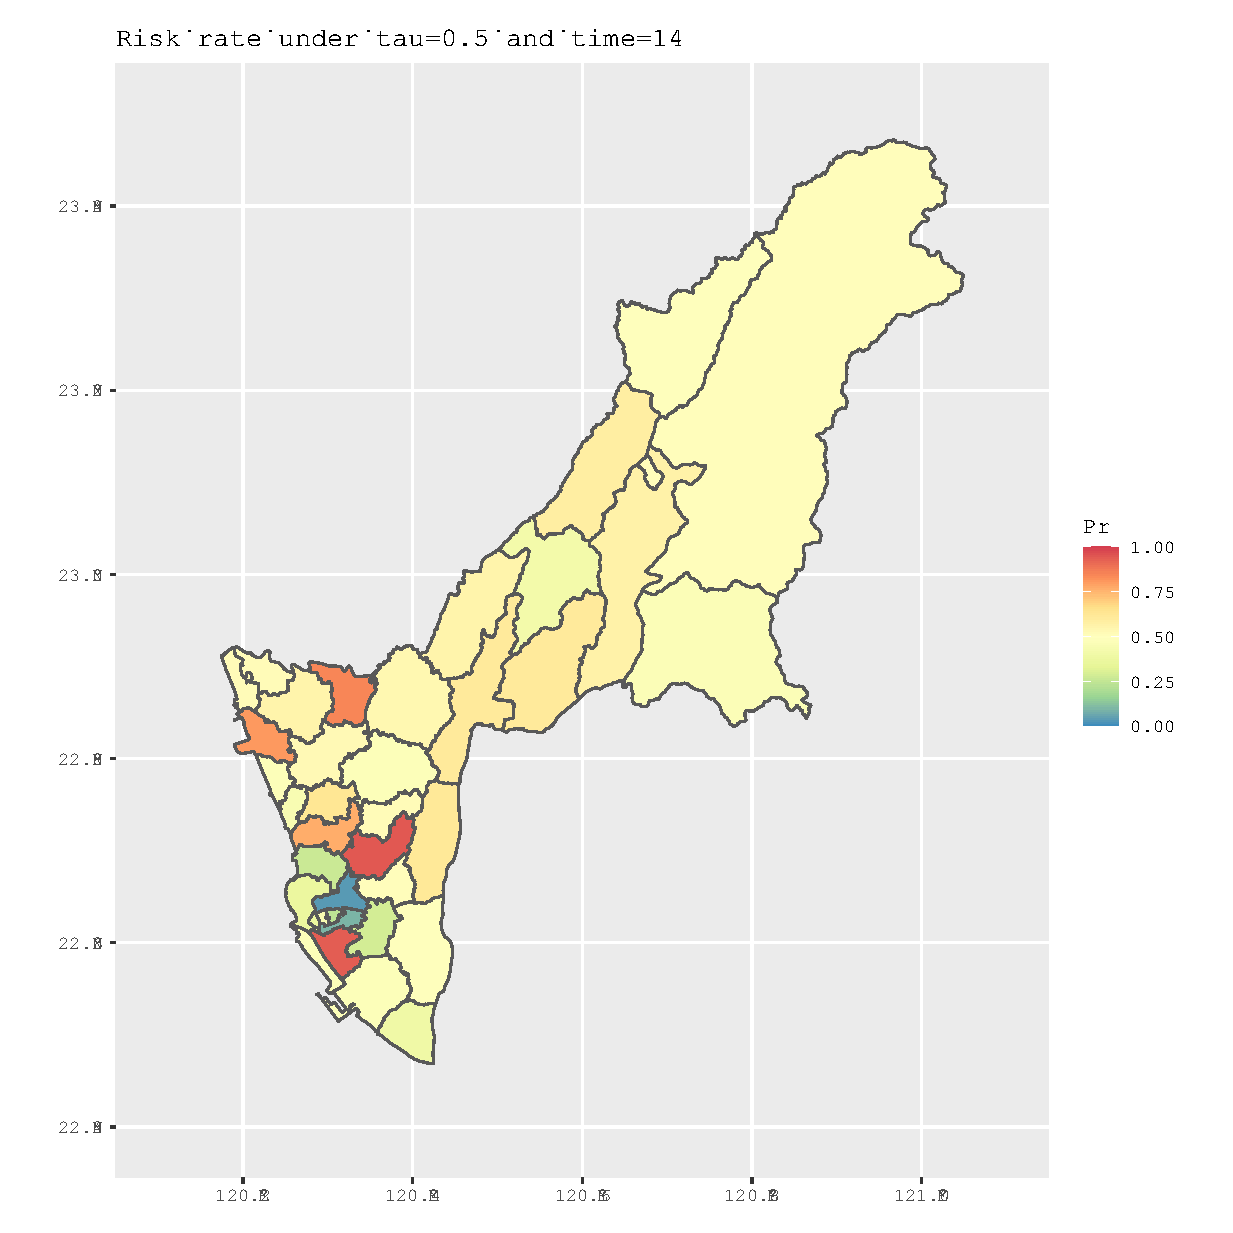
\includegraphics[width=0.22\paperwidth]{Risk_rate_under_tau=0.5_and_time=14.eps}}
\subfigure[第十五期]{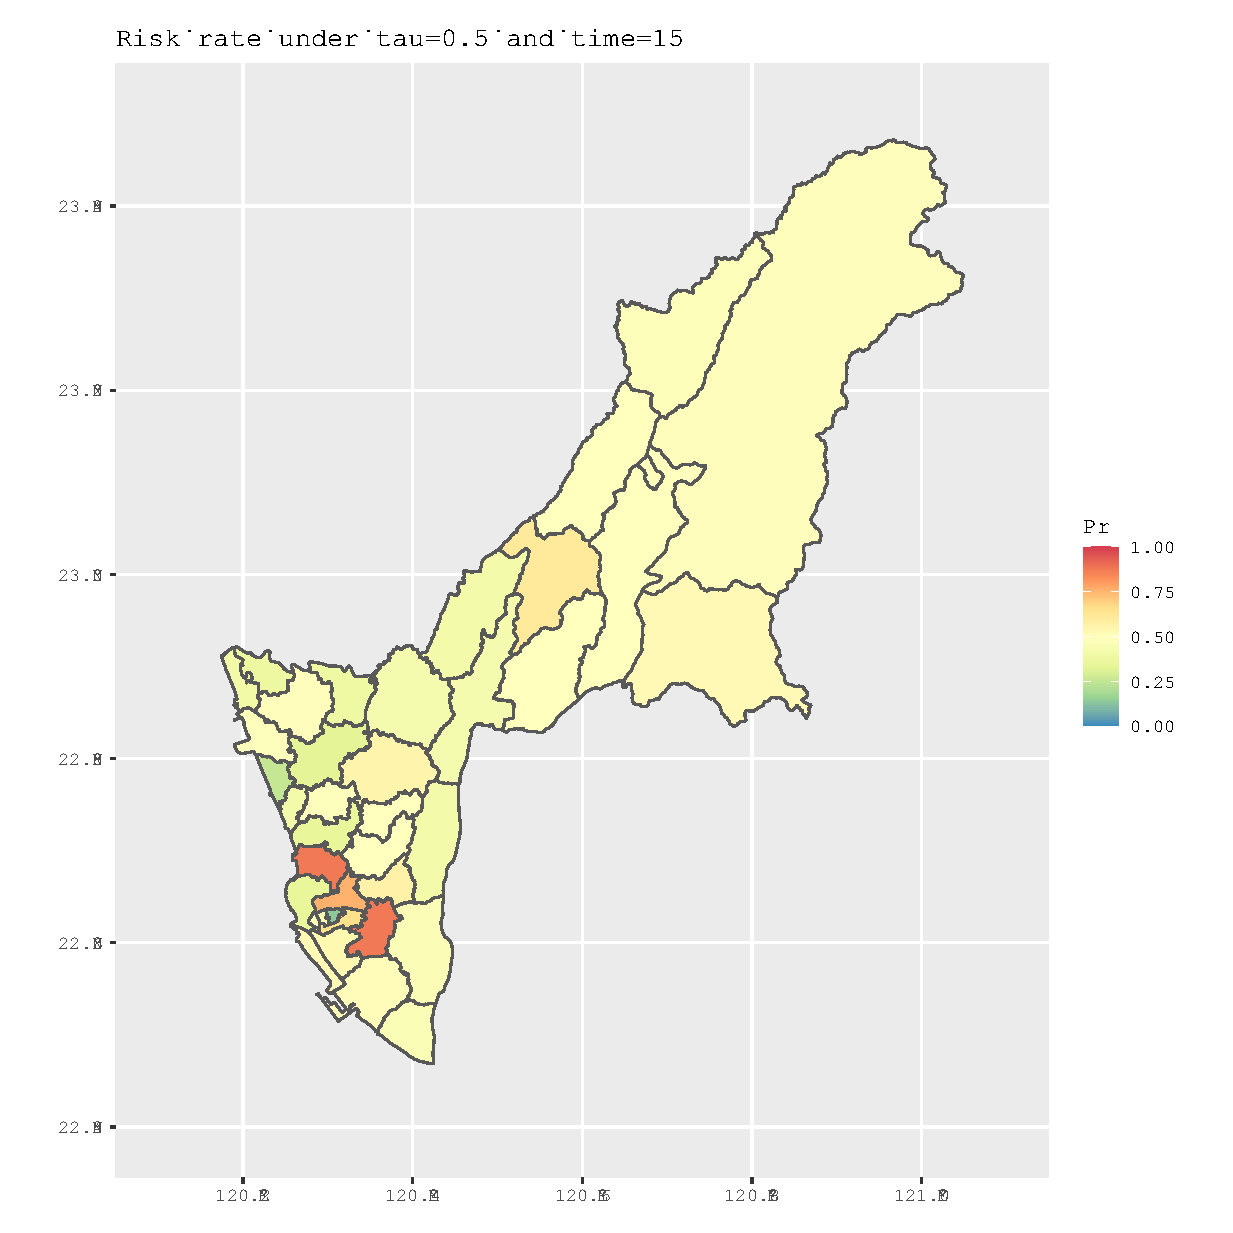
\includegraphics[width=0.22\paperwidth]{Risk_rate_under_tau=0.5_and_time=15.eps}}
\subfigure[第十六期]{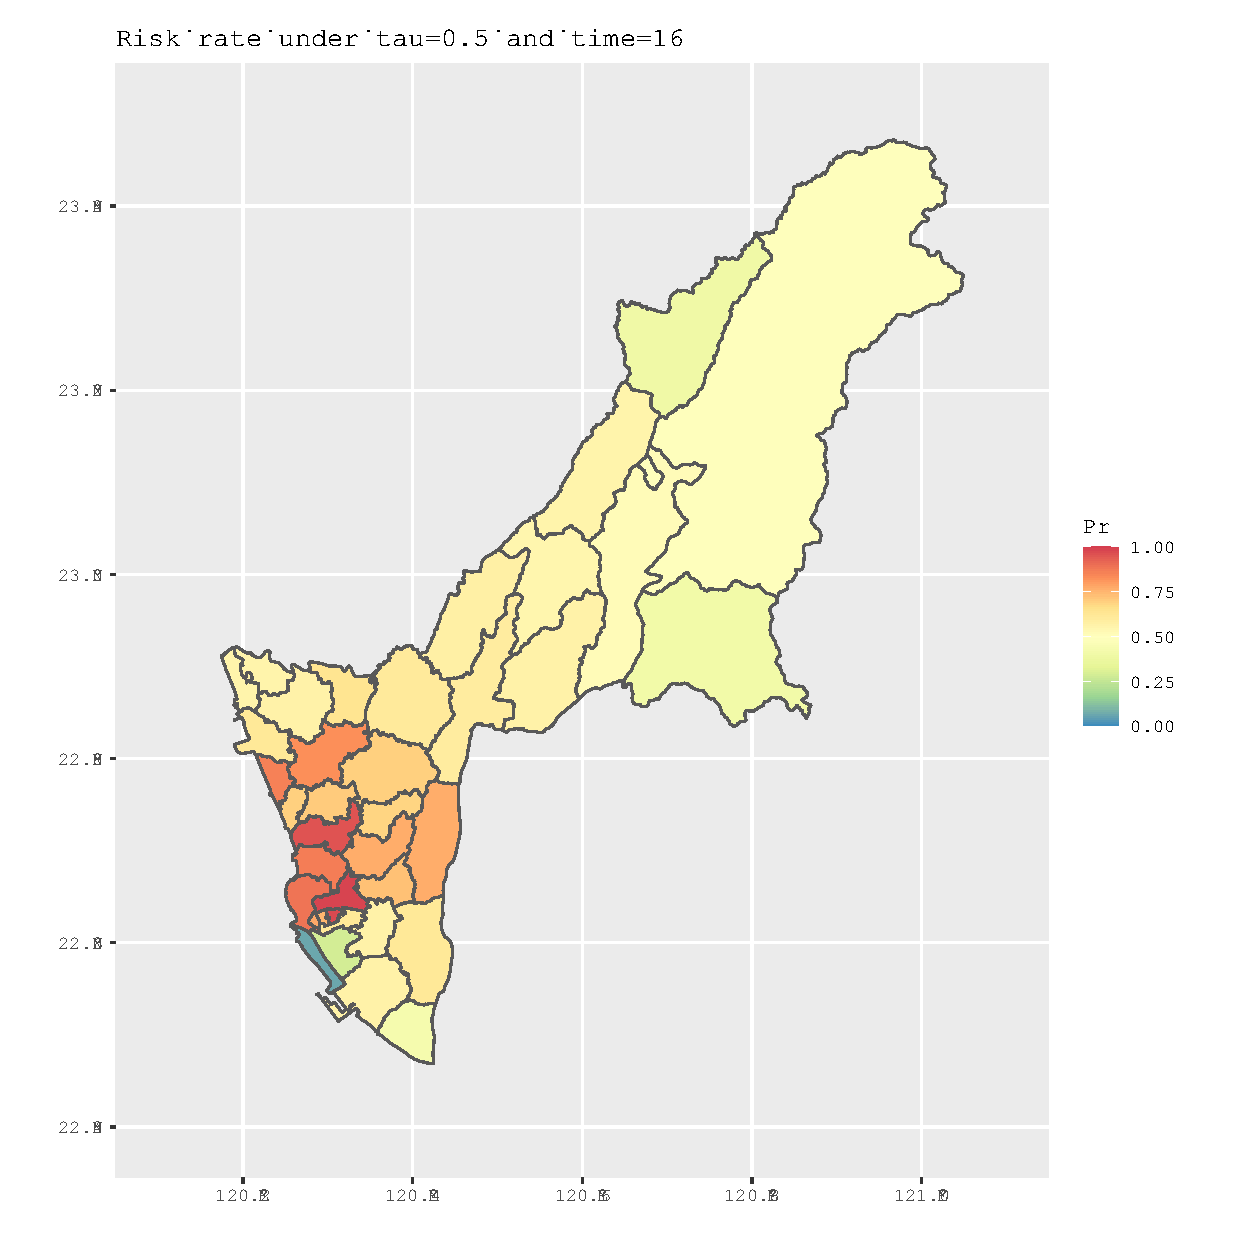
\includegraphics[width=0.22\paperwidth]{Risk_rate_under_tau=0.5_and_time=16.eps}} \\
\subfigure[第十七期]{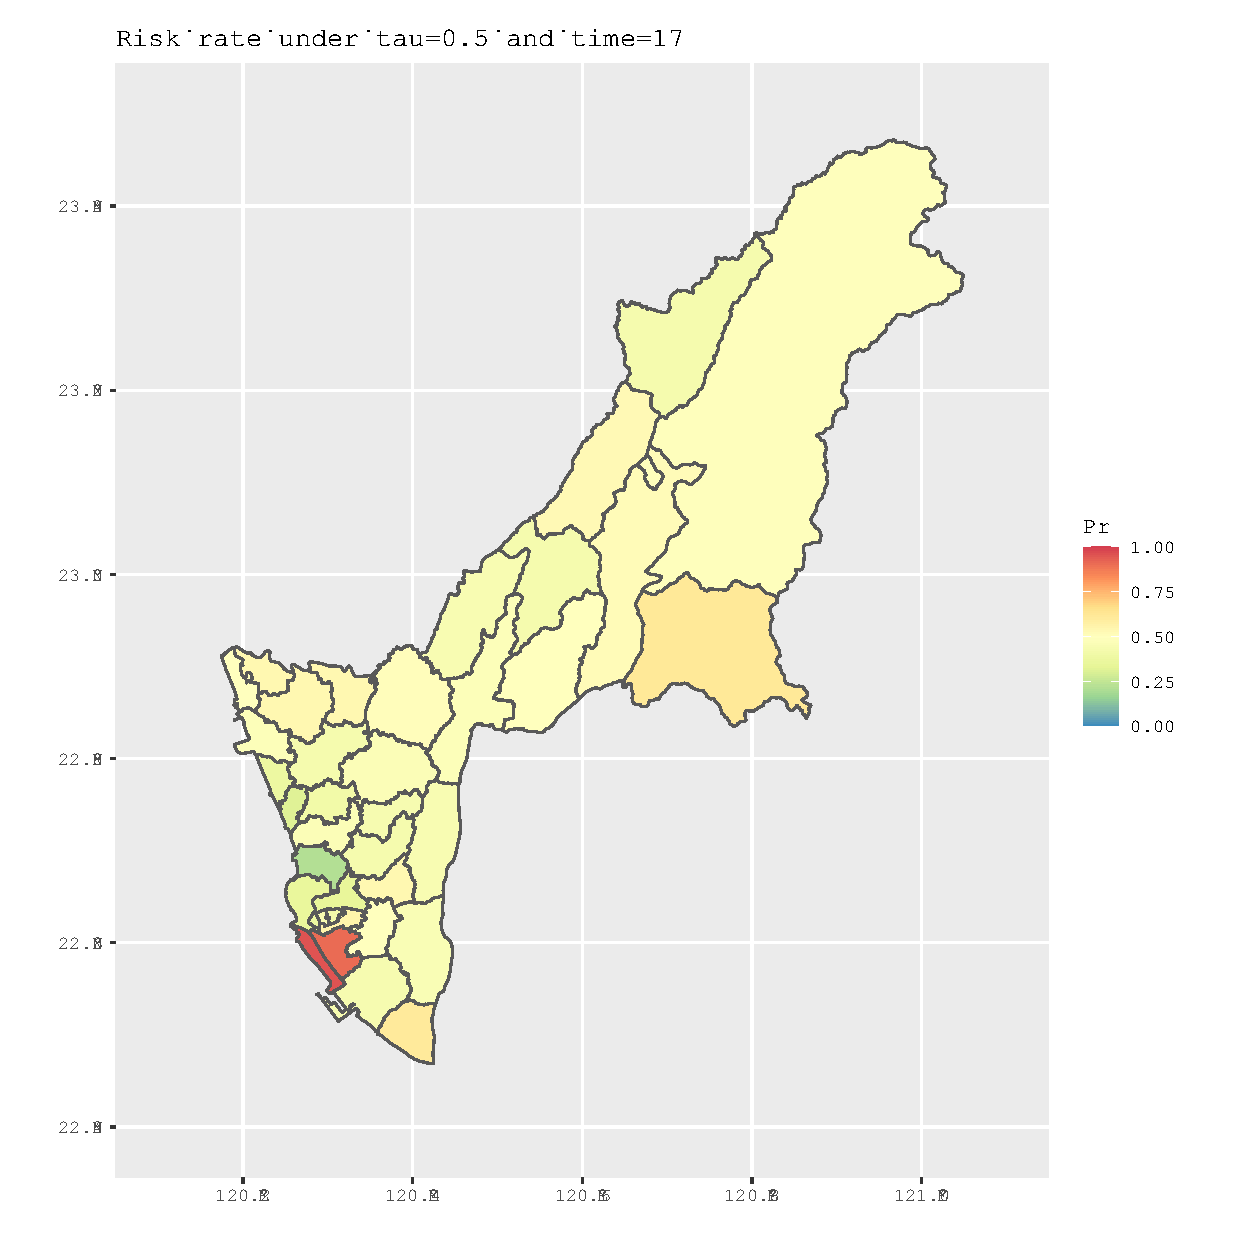
\includegraphics[width=0.22\paperwidth]{Risk_rate_under_tau=0.5_and_time=17.eps}}
\subfigure[第十八期]{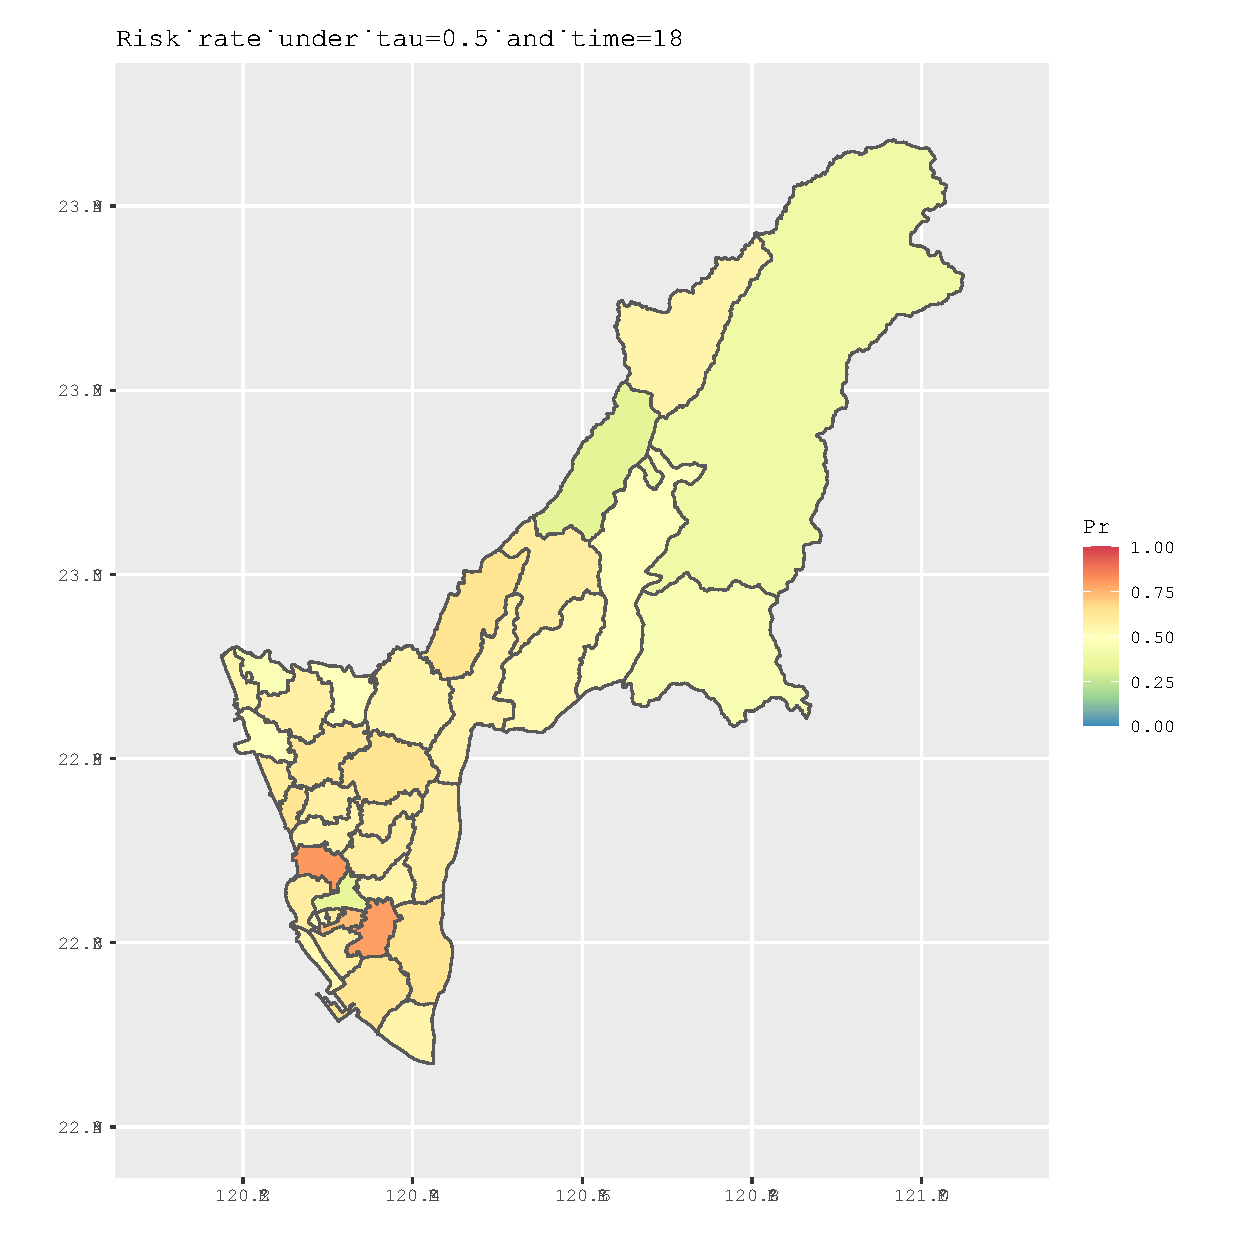
\includegraphics[width=0.22\paperwidth]{Risk_rate_under_tau=0.5_and_time=18.eps}}
\subfigure[第十九期]{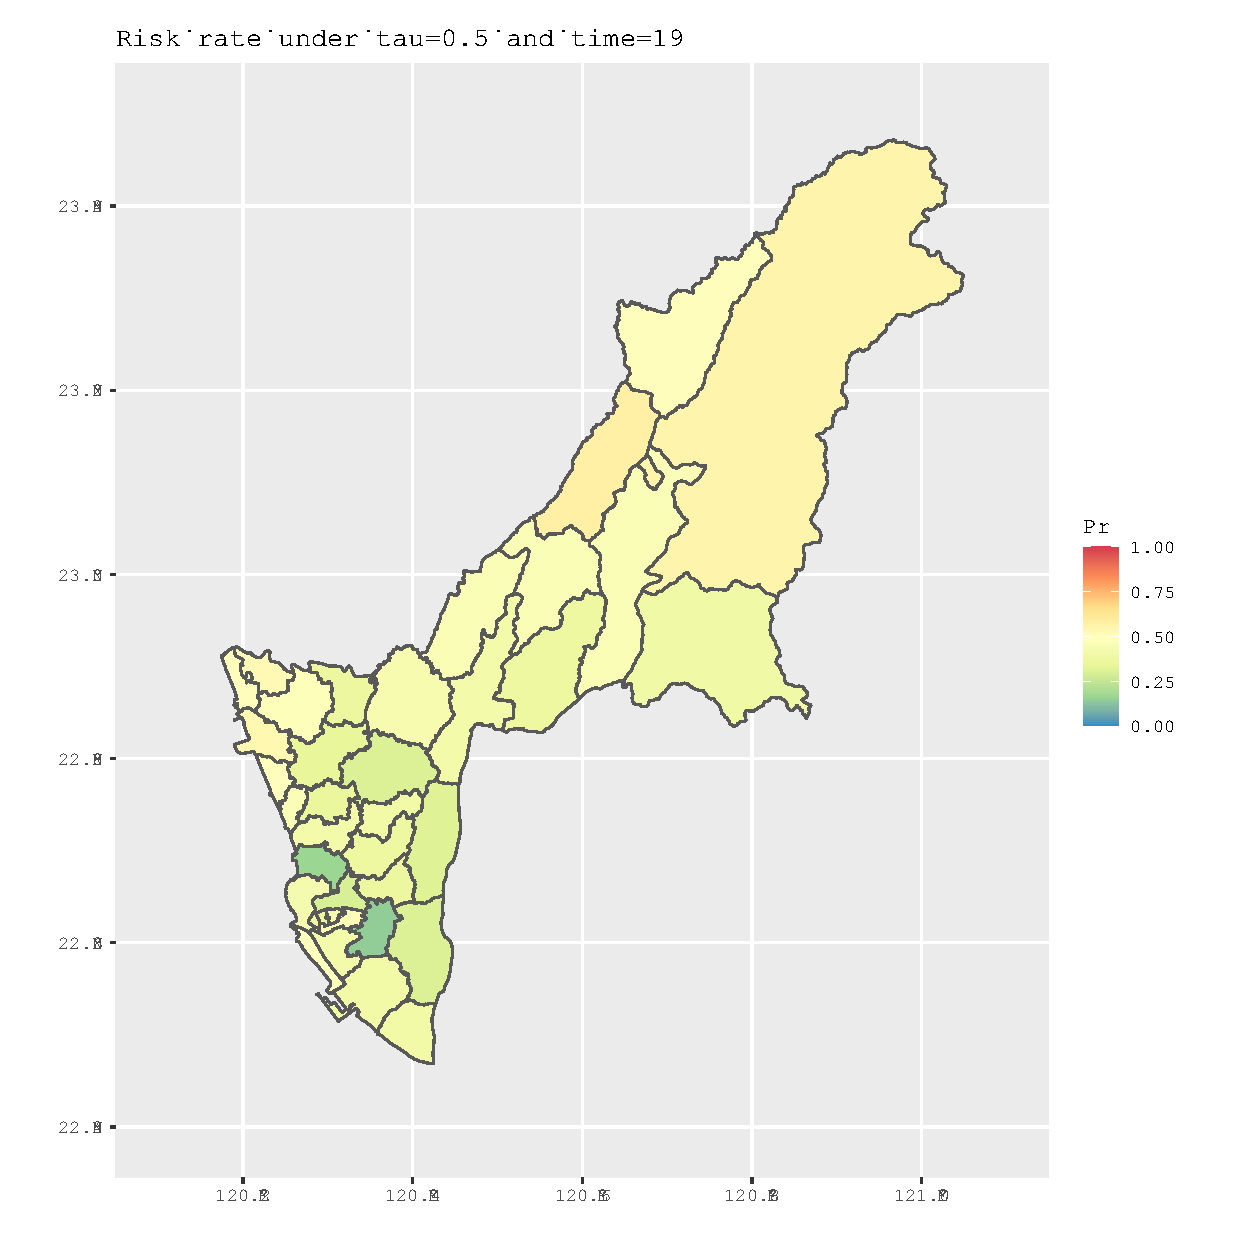
\includegraphics[width=0.22\paperwidth]{Risk_rate_under_tau=0.5_and_time=19.eps}}
\caption{$\tau = 0.5$ 第十一期至第十九期發生率風險機率圖}
\label{Fig.main10}
\end{figure}

\begin{figure}[htpb]
\centering
\subfigure[第一期]{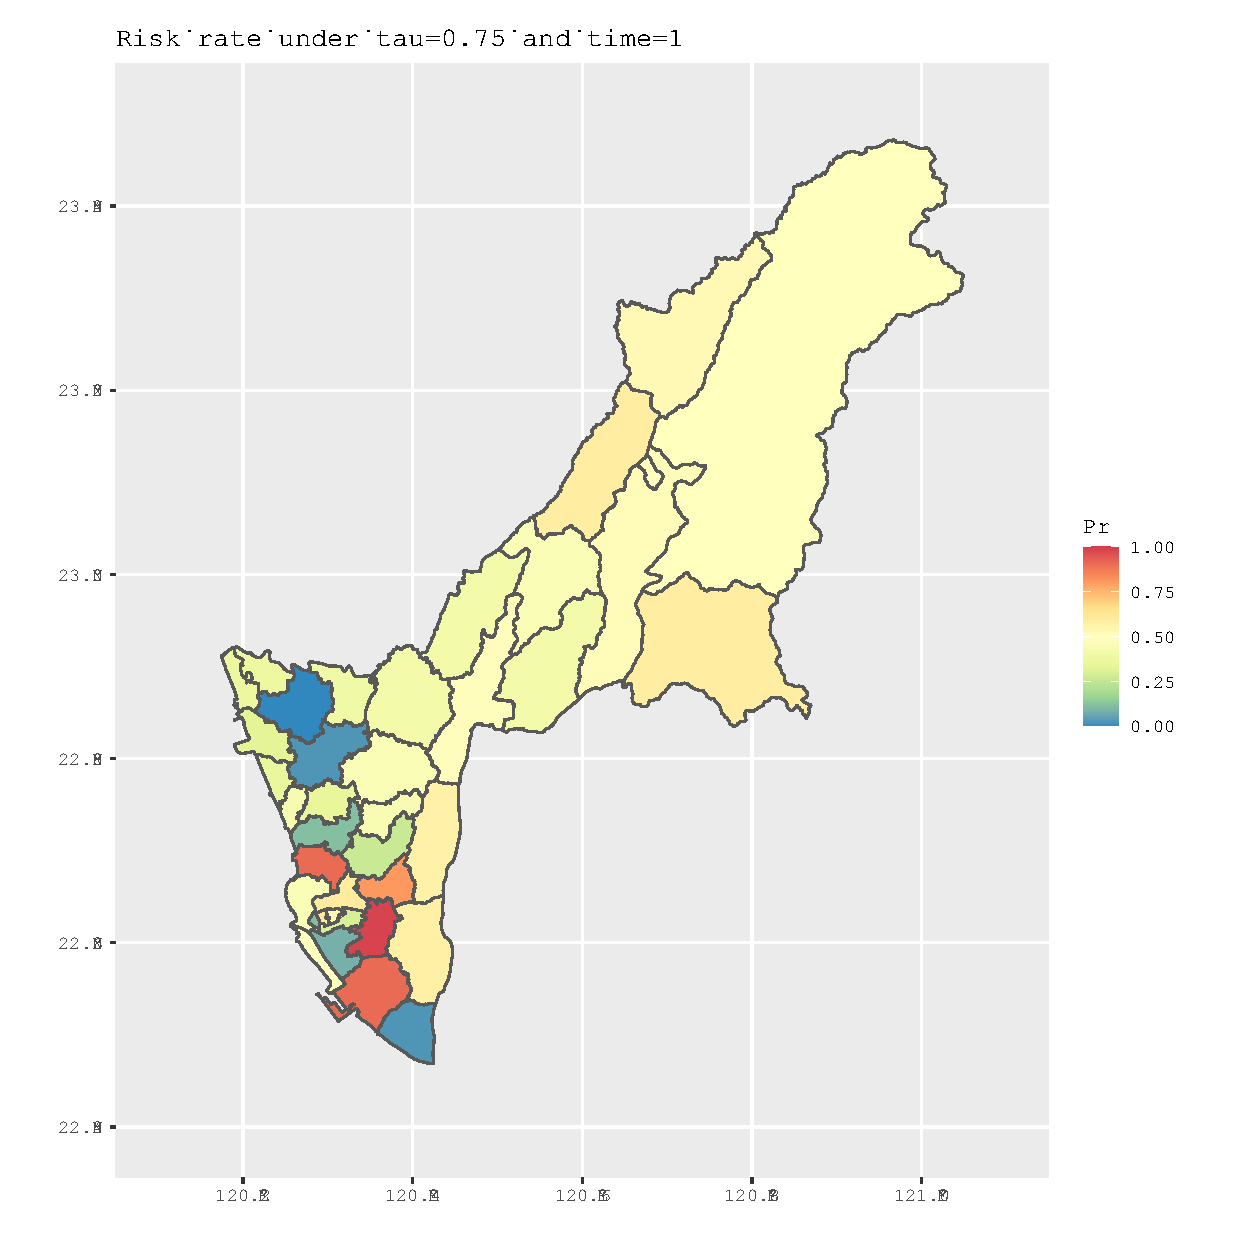
\includegraphics[width=0.22\paperwidth]{Risk_rate_under_tau=0.75_and_time=1.eps}}
\subfigure[第二期]{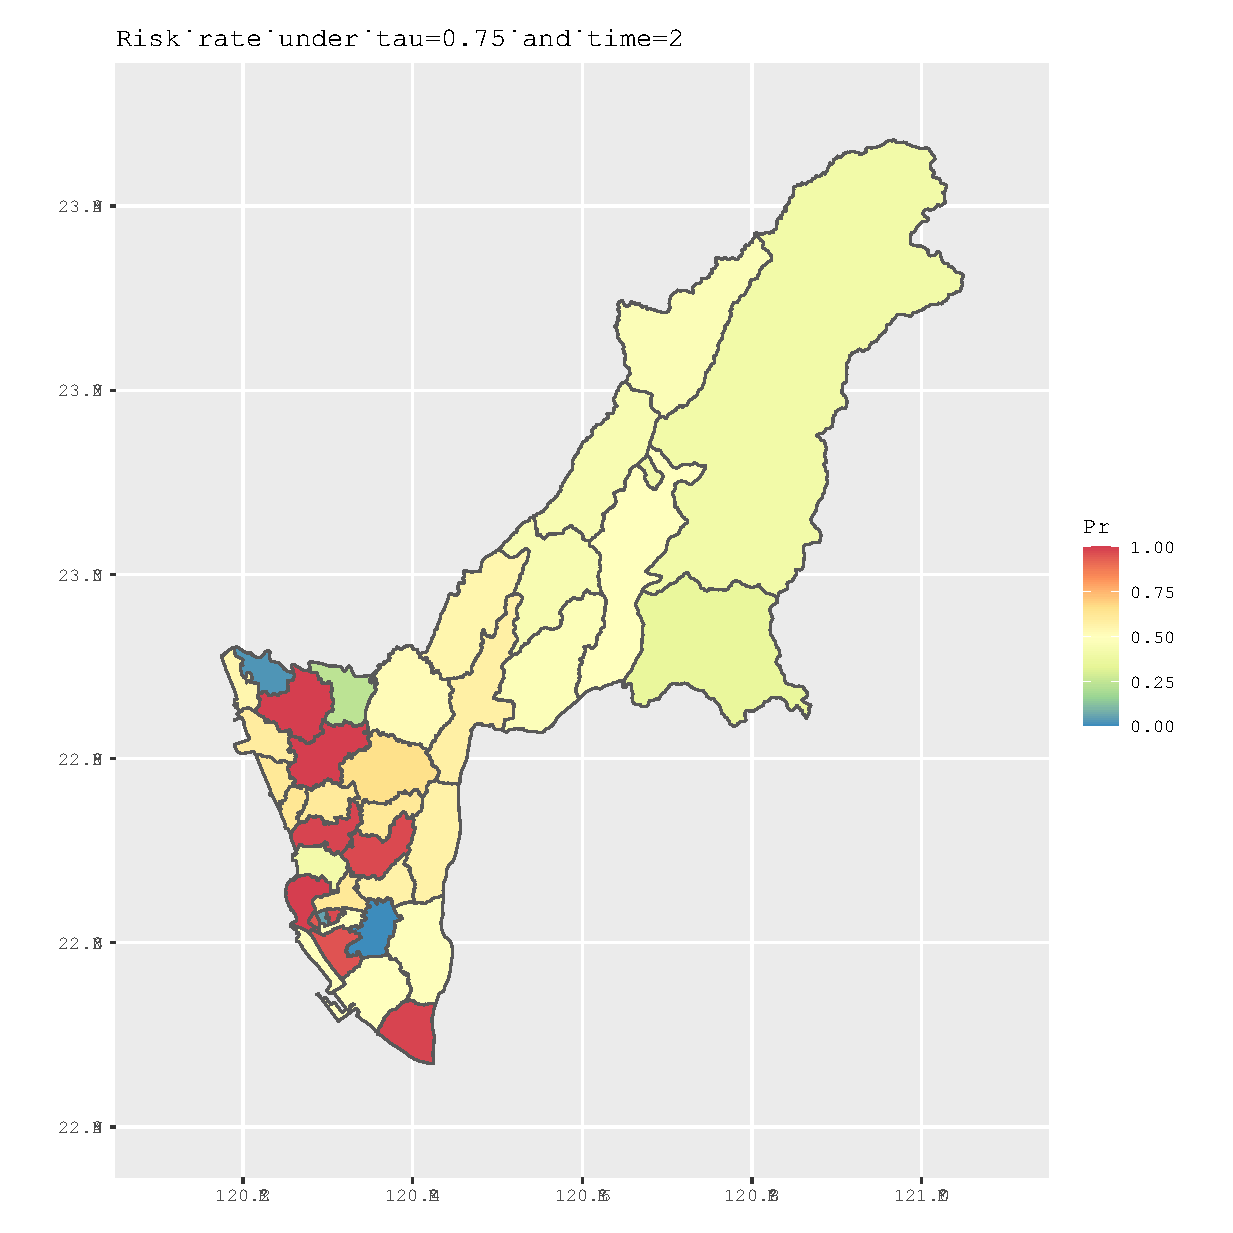
\includegraphics[width=0.22\paperwidth]{Risk_rate_under_tau=0.75_and_time=2.eps}}
\subfigure[第三期]{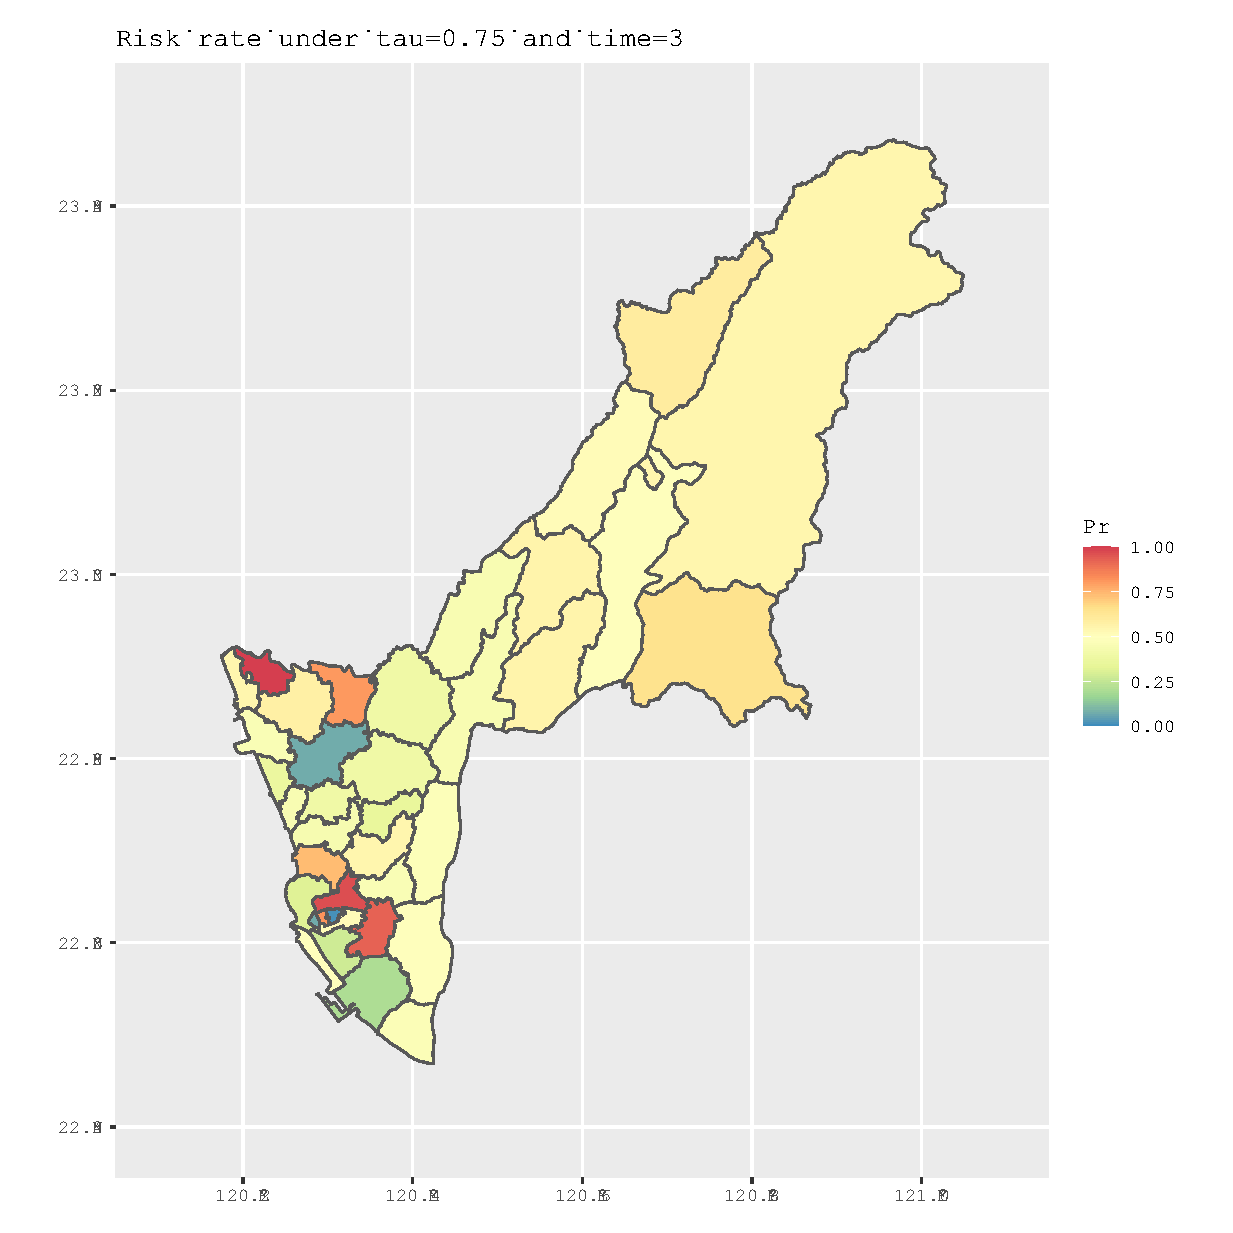
\includegraphics[width=0.22\paperwidth]{Risk_rate_under_tau=0.75_and_time=3.eps}} \\
\subfigure[第四期]{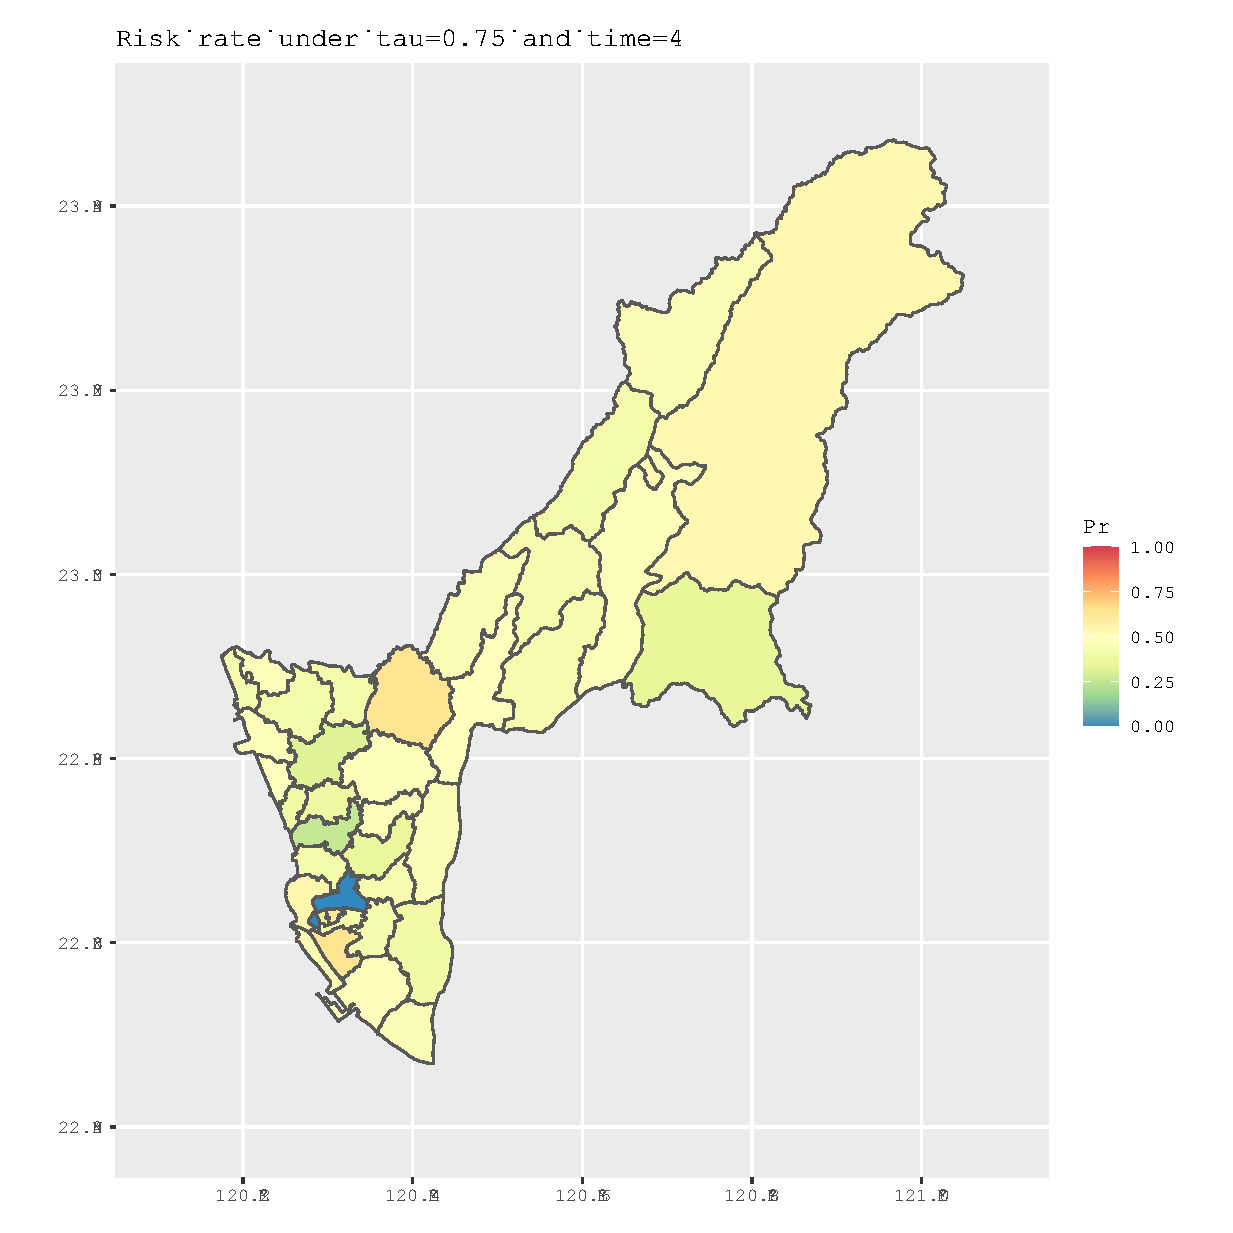
\includegraphics[width=0.22\paperwidth]{Risk_rate_under_tau=0.75_and_time=4.eps}}
\subfigure[第五期]{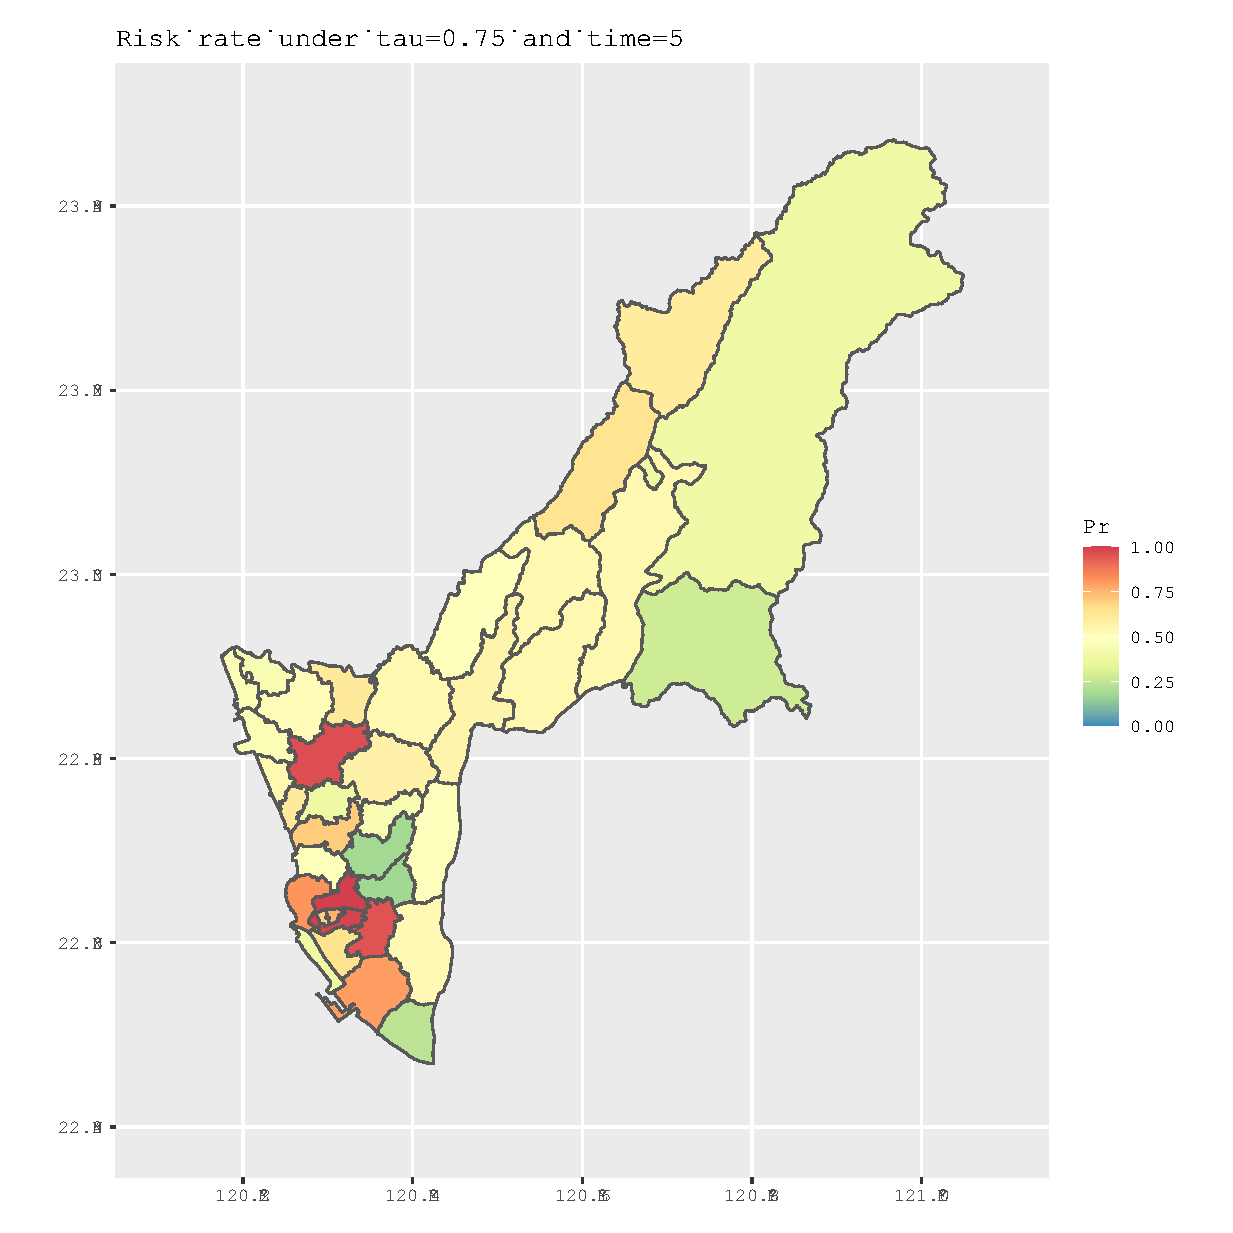
\includegraphics[width=0.22\paperwidth]{Risk_rate_under_tau=0.75_and_time=5.eps}}
\subfigure[第六期]{\includegraphics[width=0.22\paperwidth]{Risk_rate_under_tau=0.75_and_time=6.eps}} \\
\subfigure[第七期]{\includegraphics[width=0.22\paperwidth]{Risk_rate_under_tau=0.75_and_time=7.eps}}
\subfigure[第八期]{\includegraphics[width=0.22\paperwidth]{Risk_rate_under_tau=0.75_and_time=8.eps}}
\subfigure[第九期]{\includegraphics[width=0.22\paperwidth]{Risk_rate_under_tau=0.75_and_time=9.eps}} \\
\subfigure[第十期]{\includegraphics[width=0.22\paperwidth]{Risk_rate_under_tau=0.75_and_time=10.eps}}
\caption{$\tau = 0.75$ 第一期至第十期發生率風險機率圖}
\label{Fig.main11}
\end{figure}

\begin{figure}[htpb]
\centering
\subfigure[第十一期]{\includegraphics[width=0.22\paperwidth]{Risk_rate_under_tau=0.75_and_time=11.eps}}
\subfigure[第十二期]{\includegraphics[width=0.22\paperwidth]{Risk_rate_under_tau=0.75_and_time=12.eps}}
\subfigure[第十三期]{\includegraphics[width=0.22\paperwidth]{Risk_rate_under_tau=0.75_and_time=13.eps}}\\
\subfigure[第十四期]{\includegraphics[width=0.22\paperwidth]{Risk_rate_under_tau=0.75_and_time=14.eps}}
\subfigure[第十五期]{\includegraphics[width=0.22\paperwidth]{Risk_rate_under_tau=0.75_and_time=15.eps}}
\subfigure[第十六期]{\includegraphics[width=0.22\paperwidth]{Risk_rate_under_tau=0.75_and_time=16.eps}} \\
\subfigure[第十七期]{\includegraphics[width=0.22\paperwidth]{Risk_rate_under_tau=0.75_and_time=17.eps}}
\subfigure[第十八期]{\includegraphics[width=0.22\paperwidth]{Risk_rate_under_tau=0.75_and_time=18.eps}}
\subfigure[第十九期]{\includegraphics[width=0.22\paperwidth]{Risk_rate_under_tau=0.75_and_time=19.eps}}
\caption{$\tau = 0.75$ 第十一期至第十九期發生率風險機率圖}
\label{Fig.main12}
\end{figure}

\newpage
%----------------------------------------------------------------------------------------------------------
\section{總結}\label{sec:5}
本論文面對含有時空相關性的零膨脹資料,考慮以不同時間點的隨機效應項對零膨脹卜瓦松模型進行聯合建模,並使用分位數迴歸分析在不同分位數之下解釋變數對結構零的影響,
後續透過馬可夫鏈蒙地卡羅生成近似獨立後驗樣本分析各參數與隨機效應項。
在 MCMC 過程中,對於參數的完全條件分配服從已知分配者採用 Gibbs 演算法,為未知分配者則使用 M-H 演算法生成,並根據參數的交換率調整提議函數的變異數,避免參數在更新過程中發散。
最終模型達到了可以分析具有時間趨勢與空間相關性的零膨脹資料的效果,與不同模型相比具有更好的預測能力。

我們在實際資料以高雄市吸食快樂丸案件發生數進行分析,可以發現對於此筆時空零膨脹資料,本論文提出的時空零膨脹模型相較其他零膨脹模型有著更好的預測結果。
迴歸係數的估計結果透過所生成各參數後驗樣本的 $95\%$ 和 $2.5\%$ 百分位數是否同號來判斷是否顯著,並且解釋變數的顯著性依不同分位數而有所改變,
而解釋變數中每人分得警政單位個數和性別比在三個分位數的結果中都是顯著的,因此我們判斷這兩個解釋變數對吸食快樂丸案件數具有顯著影響。

根據分析結果,對於具有時間趨勢與空間相關性的零膨脹資料,本論文所提出的空間零膨脹卜瓦松迴歸模型對不同時間點的隨機效應項聯合建模,使模型具有良好的配適效果。
而在選取解釋變數時,可以參考與毒品相關的文獻,將不同的吸食毒品重要因子納入模型,使模型預測能力更加完善。
另外,本論文的模型在進行 MCMC 迭代時須將所有解釋變數加入,若要增加或減少解釋變數需重新估計,這將耗費大量運算時間,因此未來可以嘗試在此方向進行探討。

\newpage
%----------------------------------------------------------------------------------------------------------
\section*{參考文獻}
\addcontentsline{toc}{section}{參考文獻}
\begin{enumerate}
\item[{[1]}] Agarwal, D. K., Gelfand, A. E., \& Citron-Pousty, S. (2002). Zero-inflated models with application to spatial count data. \emph{Environmental and Ecological Statistics}, $\mathit{9}$(4), 341-355.
\item[{[2]}] Chen, C. S., \& Yang, H. D. (2011). A joint modeling approach for spatial earthquake risk variations. \emph{Journal of Applied Statistics}, $\mathit{38}$(8), 1733-1741.
\item[{[3]}] Chen, C. W. S., Gerlach, R., \& So, M. K. P. (2006). Comparison of nonnested asymmetric heteroskedastic models. \emph{Computational Statistics \& Data Analysis}, $\mathit{51}$, 2164–2178.
\item[{[4]}] Chib, S., \& Greenberg, E. (1995). Understanding the Metropolis-Hastings algorithm. \emph{The American Statistician}, $\mathit{49}$(4), 327-335.
\item[{[5]}] Christensen, O., \&  Waagepetersen, R. (2002). Bayesian prediction of spatial count data using generalized linear mixed models. \emph{Biometrics}, $\mathit{58}$, 280-300.
\item[{[6]}] Cressie, N. (2015). \emph{Statistics for Spatial Data}. John Wiley \& Sons.
\item[{[7]}] Fatti, L. P., Senaoana, E. M., \& Thompson, M. L. (1998). Bayesian updating in reference centile charts. \emph{Journal of the Royal Statistical Society: Series A (Statistics in Society)}, $\mathit{161}$(1), 103-115.
\item[{[8]}] Geman, S., \& Geman, D. (1984). Stochastic relaxation, Gibbs distributions, and the Bayesian restoration of images. \emph{IEEE Transactions on Pattern Analysis and Machine Intelligence}, $\mathit{6}$(6), 721-741.
\item[{[9]}] Ghosh, S. K., Mukhopadhyay, P., and Lu, J. C. (1998). Bayesian analysis of zero-inflated regression models. Technical Report, Department of Statistics, North Carolina State University.
\item[{[10]}] Greene, W. H. (1994). Accounting for excess zeros and sample selection in poisson and negative binomial regression models.  Technical Report, New York University.
\item[{[11]}] Hastings, W. K. (1970). Monte Carlo sampling methods using Markov chains and their applications. \emph{Biometrika}, $\mathit{57}$(1), 97-109.
\item[{[12]}] Heilbron, D. C. (1989). Generalized linear models for altered zero probabilities and overdispersion in count data. Technical Report, University of California, Department of Epidemiology and Biostatistics, San Francisco.
\item[{[13]}] Heilbron, D. C. (1994). Zero-altered and other regression models for count data with added zeros. \emph{Biometrical Journal}, $\mathit{36}$, 531-547.
\item[{[14]}] Kozumi, H. and Kobayashi, G. (2011). Gibbs sampling methods for Bayesian quantile regression. \emph{Journal of Statistical Computation and Simulation}, $\mathit{81}$(11),1565-1578.
\item[{[15]}] Lambert, D. (1992). Zero-inflated Poisson regression, with an application to defects in manufacturing. \emph{Technometrics}, $\mathit{34}$(1), 1-14.
\item[{[16]}] Metropolis, N., Rosenbluth, A. W., Rosenbluth, M. N., Teller, A. H., \& Teller, E. (1953). Equation of state calculations by fast computing machines. \emph{The Journal of Chemical Physics}, $\mathit{21}$(6), 1087-1092.
\item[{[17]}] Mullahy, J. (1986). Specification and testing of some modified count data models. \emph{Journal of Econometrics}, $\mathit{33}$, 341-365.
\item[{[18]}] NIDA. (2022). Sex and Gender Differences in Substance Use. Retrieved from https://nida.nih.gov/publications/research-reports/substance-use-in-women/sex-gender-differences-in-substance-use.
\item[{[19]}] Parry, S. (2018). To Offset or Not: Using Offsets in Count Models. \emph{StatNews\# 94, Ithaca, NY, Cornell University.}
\item[{[20]}] Yu, K., \& Moyeed, R. A. (2001). Bayesian quantile regression. \emph{Statistics and Probability Letters}, $\mathit{54}$(4), 437-447.
\item[{[21]}] 蔡奇秀. (2006). 影響毒品犯罪率因素之實證研究. 成功大學高階管理碩士在職專班 (EMBA) 學位論文, 1-125.
\end{enumerate}

\newpage
%----------------------------------------------------------------------------------------------------------
\section*{附錄}
\addcontentsline{toc}{section}{附錄}
\noindent
推導各參數與隨機效應項的完全條件分配過程,
本研究所使用之 inverse gamma 分配的機率密度函數為:
 \begin{gather*}
 \setlength\abovedisplayskip{25pt}
 \setlength\belowdisplayskip{25pt}
X \sim IG(a,b) \\[3mm]
f(x|a,b) = \frac{b^a}{\Gamma(a)} \left( \frac{1}{x} \right) ^{a+1} e^{\frac{-b}{x}} ,x > 0 \\[3mm]
mean : \frac{b}{a-1} \quad for \quad a > 1 \\[3mm]
variance : \frac{b^2}{(a-1)^2(a-2)} \quad for \quad a > 2
 \end{gather*}
聯合後驗分配:
 \begin{align*}
 \setlength\abovedisplayskip{25pt}
 \setlength\belowdisplayskip{25pt}
  P & \left(\bm{\theta},\bm{z},\bm{u},\bm{\delta}_0,\bm{\delta}_1,\dots,\bm{\delta}_T|\bm{Y_1},\dots,\bm{Y_T}\right)  \\[3mm]
   \propto &  P(\bm{Y_1},\dots,\bm{Y_T}|\bm{\theta},\bm{z},\bm{u},\bm{\delta}_0,\bm{\delta}_1,\dots,\bm{\delta}_T) \times P(\bm{\theta},\bm{z},\bm{u},\bm{\delta}_0,\bm{\delta}_1,\dots,\bm{\delta}_T) \\[3mm]
   = &
\prod_{t=1}^T \prod_{i=1}^NP\left(Y_{ti}|\bm{\beta},\delta_{ti},\bm{\alpha},\sigma_R,z_i,u_i\right)\prod_{t=1}^TP\left(\bm{\delta_t}|\sigma_t^2,\phi_t,\bm{\delta_0}\right) P\left(\bm{\delta_0}|\sigma_0^2,\phi_0,\bm{\eta}\right) \prod_{i=1}^NP\left(z_i\right) \prod_{i=1}^NP\left(u_i\right) \pi\left(\theta\right) \\[3mm]
   = &
\prod_{t=1}^T\prod_{i=1}^N \left\{ \left( \frac{1}{1+e^{-(\bm{W^\prime}\bm{\alpha}+\sigma_R(\zeta z_i+\xi \sqrt[]{z_i} u_i))}} \right)I\left\{ Y_{ti} = 0\right\} \right.\\[3mm]
& + \left. \left(1-\left( \frac{1}{1+e^{-(\bm{W^\prime}\bm{\alpha}+\sigma_R(\zeta z_i+\xi \sqrt[]{z_i} u_i))}} \right)\right)\frac{e^{-\left(e^{\bm{X_{ti}^\prime\bm{\beta}}+\delta_{ti}}\right)}e^{(\bm{X_{ti}^\prime\bm{\beta}}+\delta_{ti})y_{ti}}}{y_{ti}!}\right\}\\[3mm]
  & \times
\prod_{t=1}^T\left[ \left( det\left(\sigma_t^2(\bm{I_N}-\phi_t\bm{C})^{-1}\right) \right)^{-\frac{1}{2}} e^{ -\frac{1}{2\sigma_t^2}(\bm{\delta_t}-\bm{\delta_0})^\prime(\bm{I_N}-\phi_t\bm{C})(\bm{\delta_t}-\bm{\delta_0})} \right]\\[3mm]
  & \times
\left( det\left(\sigma_0^2(\bm{I_N}-\phi_0\bm{C})^{-1}\right) \right)^{-\frac{1}{2}} e^{ -\frac{1}{2\sigma_0^2}(\bm{\delta_0}-\bm{\eta})^\prime(\bm{I_N}-\phi_0\bm{C})(\bm{\delta_0}-\bm{\eta})}\\[3mm]
  & \times
\prod_{i=1}^N e^{-z_i} \times \prod_{i=1}^N e^{-\frac{u_i^2}{2}} \times \prod_{i=1}^N \left[ \left(2 \pi f_i^2 \right)^{-\frac{1}{2}}e^{ -\frac{1}{2 f_i^2}(\eta_i-e_i)^2}\right] \\[3mm]
  & \times
\prod_{k=0}^K \left[ \frac{1}{\sqrt{2\pi d_k^2}}e^{-\frac{(\beta_k-c_k)^2}{2d_k^2}}\right] \times \frac{b_0^{a_0}}{\Gamma(a_0)}\left(\frac{1}{\sigma_0^2}\right)^{a_0+1}e^{\frac{-b_0}{\sigma_0^2}} \\[3mm]
  & \times
\prod_{t=1}^T\left[ \frac{b_t^{a_t}}{\Gamma(a_t)}\left(\frac{1}{\sigma_t^2}\right)^{a_t+1}\right]e^{\frac{-b_t}{\sigma_t^2}} \times \frac{1}{\phi_{max}} \times \prod_{t=1}^T\frac{1}{\phi_{max}} \times \prod_{l=0}^L\frac{1}{h_l-g_l} \\[3mm]
  & \times
\frac{b_R^{a_R}}{\Gamma(a_R)}\left(\frac{1}{\sigma_R}\right)^{a_R+1}e^{\frac{-b_R}{\sigma_R}}\\[3mm]
  \propto &
\prod_{t=1}^T\prod_{i=1}^N \left\{ \left( \frac{1}{1+e^{-(\bm{W^\prime}\bm{\alpha}+\sigma_R(\zeta z_i+\xi \sqrt[]{z_i} u_i))}} \right)I\left\{ Y_{ti} = 0\right\} \right.\\[3mm]
& + \left. \left(1-\left( \frac{1}{1+e^{-(\bm{W^\prime}\bm{\alpha}+\sigma_R(\zeta z_i+\xi \sqrt[]{z_i} u_i))}} \right)\right)\frac{e^{-\left(e^{\bm{X_{ti}^\prime\bm{\beta}}+\delta_{ti}}\right)}e^{(\bm{X_{ti}^\prime\bm{\beta}}+\delta_{ti})y_{ti}}}{y_{ti}!}\right\}      \\[3mm]
  & \times \left( det\left(\sigma_0^2(\bm{I_N}-\phi_0\bm{C})^{-1}\right) \right)^{-\frac{1}{2}} \times \left(\frac{1}{\sigma_0^2}\right)^{a_0+1} \times \left(\frac{1}{\sigma_R}\right)^{a_R+1} \\[3mm]
  & \times
\prod_{t=1}^T \left(\left(\frac{1}{\sigma_t^2}\right)^{a_t+1}\left( det\left(\sigma_t^2(\bm{I_N}-\phi_t\bm{C})^{-1}\right) \right)^{-\frac{1}{2}}\right)    \\[3mm]
  & \times
 exp \left\{-\left( \sum_{t=1}^T\left(\frac{b_t}{\sigma_t^2}+\frac{1}{2\sigma_t^2}(\bm{\delta_t}-\bm{\delta_0})^\prime(\bm{I_N}-\phi_t\bm{C})(\bm{\delta_t}-\bm{\delta_0})\right) + \sum_{k=0}^K\left[\frac{(\beta_k-c_k)^2}{2d_k^2}\right] \right.\right.\\[3mm]
& \left.\left. + \sum_{i=1}^N \left( z_i + \frac{u_i^2}{2}+\frac{(\eta_i-e_i)^2}{2 f_i^2}\right) + \frac{b_R}{\sigma_R}+\frac{b_0}{\sigma_0^2}+\left[\frac{1}{2\sigma_0^2}(\bm{\delta_0}-\bm{\eta})^\prime(\bm{I_N}-\phi_0\bm{C})(\bm{\delta_0}-\bm{\eta})\right]\right)\right\}.
 \end{align*}
計算各參數與隨機效應項的完全條件分配,以 $\beta_k$ 為例:
 \begin{align*}
 \setlength\abovedisplayskip{25pt}
 \setlength\belowdisplayskip{25pt}
 P & (\beta_k|\bm{\theta}_{(-\beta_k)},\bm{\chi}) \\[3mm]
  \propto &
 P(\bm{Y_1},\dots,\bm{Y_T}|\bm{\theta},\bm{z},\bm{u},\bm{\delta}_0,\bm{\delta}_1,\dots,\bm{\delta}_T) \times
 P(\bm{\theta},\bm{z},\bm{u},\bm{\delta}_0,\bm{\delta}_1,\dots,\bm{\delta}_T) \\[3mm]
  = &
 \prod_{t=1}^T\prod_{i=1}^N P(Y_{ti}|\bm{\beta},\delta_{ti},\bm{\alpha},\sigma_R,z_i,u_i) \times \prod_{t=1}^T P(\bm{\delta_t}|\sigma_t^2,\phi_t,\bm{\delta_0}) \times P(\bm{\delta_0}|\sigma_0^2,\phi_0,\bm{\eta}) \\[3mm]
 & \times
 \prod_{i=1}^N P(z_i) \times \prod_{i=1}^N P(u_i) \times \pi(\bm{\eta}) \times \pi(\bm{\beta}) \times \prod_{t=0}^T \pi(\sigma_t^2) \times \prod_{t=0}^T \pi(\phi_t) \times \pi(\bm{\alpha}) \times \pi(\sigma_R) \\[3mm]
  \propto &
 \prod_{t=1}^T \prod_{i=1}^N P(Y_{ti}|\bm{\beta},\delta_{ti},\bm{\alpha},\sigma_R,z_i,u_i) \times \pi(\beta_k) \\
 \end{align*}
同上述方法,以此類推其他參數與隨機效應項:%,引入符號 $\bm{\theta}_{(-\gamma)}$ 用於表示模型參數向量移除任一模型參數 $\gamma$ 後之模型參數向量:
 \begin{align*}
 \setlength\abovedisplayskip{25pt}
 \setlength\belowdisplayskip{25pt}
  P & (\phi_t|\bm{\theta}_{(-\phi_t)},\bm{\chi}) \propto  P(\bm{\delta_{t}}|\sigma_t^2,\phi_t,\bm{\delta_0}) \times \pi(\phi_t) \\[3mm]
  P & (\phi_0|\bm{\theta}_{(-\phi_0)},\bm{\chi}) \propto  P(\bm{\delta_{0}}|\sigma_0^2,\phi_0,\bm{\eta}) \times \pi(\phi_0) \\[3mm]
  P & (\sigma_t^2|\bm{\theta}_{(-\sigma_t^2)},\bm{\chi}) \propto  P(\bm{\delta_{t}}|\sigma_t^2,\phi_t,\bm{\delta_0}) \times \pi(\sigma_t^2) \\[3mm]
  P & (\sigma_0^2|\bm{\theta}_{(-\sigma_0^2)},\bm{\chi}) \propto  P(\bm{\delta_{0}}|\sigma_0^2,\phi_0,\bm{\eta}) \times \pi(\sigma_0^2) \\[3mm]
 P & (\eta_i|\bm{\theta}_{(-\eta_i)},\bm{\chi}) \propto P(\delta_{0i}|\sigma_0^2,\phi_0,\eta_i,\bm{\delta_{0(-i)}}) \times \pi(\eta_i) \\[3mm]
 P & (\alpha_l|\bm{\theta}_{(-\alpha)},\bm{\chi}) \propto \prod_{t=1}^T \prod_{i=1}^N P(Y_{ti}|\bm{\beta},\delta_{ti},\bm{\alpha},\sigma_R,z_i,u_i) \times \pi(\alpha_l) \\[3mm]
 P & (\sigma_R|\bm{\theta}_{(-\sigma_R)},\bm{\chi}) \propto \prod_{t=1}^T \prod_{i=1}^N P(Y_{ti}|\bm{\beta},\delta_{ti},\bm{\alpha},\sigma_R,z_i,u_i) \times \pi(\sigma_R) \\[3mm]
 P & (\delta_{ti}|\bm{\theta},\bm{\chi}_{(-\delta_{ti})}) \propto P(Y_{ti}|\bm{\beta},\delta_{ti},\bm{\alpha},\sigma_R,z_i,u_i) \times P(\delta_{ti}|\sigma_t^2,\phi_t,\bm{\delta_0},\bm{\delta_{t(-i)}}) \\[3mm]
 P & (\delta_{0i}|\bm{\theta},\bm{\chi}_{(-\delta_{0i})}) \propto \prod_{t=1}^T P(\delta_{ti}|\sigma_t^2,\phi_t,\bm{\delta_0},\bm{\delta_{t(-i)}}) \times P(\delta_{0i}|\sigma_0^2,\phi_0,\bm{\eta},\bm{\delta_{0(-i)}}) \\[3mm]
 P & (z_i|\bm{\theta},\bm{\chi}_{(-z_i)}) \propto \prod_{t=1}^T P(Y_{ti}|\bm{\beta},\delta_{ti},\bm{\alpha},\sigma_R,z_i,u_i) \times P(z_i) \\[3mm]
 P & (u_i|\bm{\theta},\bm{\chi}_{(-u_i)}) \propto \prod_{t=1}^T P(Y_{ti}|\bm{\beta},\delta_{ti},\bm{\alpha},\sigma_R,z_i,u_i) \times P(u_i)
 \end{align*}
各參數與隨機效應項推導過程:
%beta------------------------------------------------------------
\begin{align*}
 \setlength\abovedisplayskip{25pt}
 \setlength\belowdisplayskip{25pt}
 P & (\beta_k|\bm{\theta}_{(-\beta_k)},\bm{\chi}) \propto \prod_{t=1}^T\prod_{i=1}^N P(Y_{ti}|\bm{\beta},\delta_{ti},\bm{\alpha},\sigma_R,z_i,u_i) \times \pi(\bm{\beta}) \\[3mm]
 \propto  &
\prod_{t=1}^T\prod_{i=1}^N \left\{ p_i I \left\{ Y_{ti} = 0 \right\}+(1-p_i)\frac{e^{-\lambda_{ti}}\lambda_{ti}^{y_{ti}}}{y_{ti}!}\right\} \times \frac{1}{\sqrt{2 \pi d_k^2}}e^{-\frac{(\beta_k-c_k)^2}{2 d_k^2}} \\[3mm]
 \propto  &
\prod_{t=1}^T\prod_{i=1}^N \left\{ \left( \frac{1}{1+e^{-(\bm{W^\prime}\bm{\alpha}+\sigma_R(\zeta z_i+\xi \sqrt[]{z_i} u_i))}} \right)I\left\{ Y_{ti} = 0\right\} \right.\\[3mm]
& + \left. \left(1-\left( \frac{1}{1+e^{-(\bm{W^\prime}\bm{\alpha}+\sigma_R(\zeta z_i+\xi \sqrt[]{z_i} u_i))}} \right)\right)\frac{e^{-\left(e^{\bm{X_{ti}^\prime\bm{\beta}}+\delta_{ti}}\right)}e^{(\bm{X_{ti}^\prime\bm{\beta}}+\delta_{ti})y_{ti}}}{y_{ti}!}\right\} \times e^{-\frac{\beta_{k}^2-2\beta_k c_k}{2 d_k^2}}\\[3mm]
\\ \hspace*{\fill} \\
%phi_t----------------------------------------------------------
  P & (\phi_t|\bm{\theta}_{(-\phi_t)},\bm{\chi}) \propto  P(\bm{\delta_{t}}|\sigma_t^2,\phi_t,\bm{\delta_{0}}) \times \pi(\phi_t) \\[3mm]
 \propto &
\left(det\left(\sigma_t^2(\bm{I_N}-\phi_t\bm{C})^{-1}\right)\right)^{\left(-\frac{1}{2}\right)} e^{-\frac{(\bm{\delta_t}-\bm{\delta_{0}})^\prime(\bm{I_N}-\phi_t\bm{C})(\bm{\delta_t}-\bm{\delta_{0}})}{2\sigma_t^2}}\times\frac{1}{\phi_{max}}\\[3mm]
 \propto &
\left(det\left((\bm{I_N}-\phi_t\bm{C})^{-1}\right)\right)^{\left(-\frac{1}{2}\right)} e^{-\frac{(\bm{\delta_t}-\bm{\delta_{0}})^\prime(\bm{I_N}-\phi_t\bm{C})(\bm{\delta_t}-\bm{\delta_{0}})}{2\sigma_t^2}}\\[3mm]
 \propto &
\left(det\left((\bm{I_N}-\phi_t\bm{C})^{-1}\right)\right)^{\left(-\frac{1}{2}\right)} e^{-\frac{(\bm{\delta_t}-\bm{\delta_{0}})^\prime \bm{I_N}(\bm{\delta_t}-\bm{\delta_{0}})}{2\sigma_t^2}} \times e^{\frac{\phi_t (\bm{\delta_t}-\bm{\delta_{0}})^\prime \bm{C}(\bm{\delta_t}-\bm{\delta_{0}})}{2\sigma_t^2}}  \\[3mm]
 \propto &
 \left(det\left((\bm{I_N}-\phi_t\bm{C})^{-1}\right)\right)^{\left(-\frac{1}{2}\right)} e^{\frac{\phi_t (\bm{\delta_t}-\bm{\delta_{0}})^\prime \bm{C}(\bm{\delta_t}-\bm{\delta_{0}})}{2\sigma_t^2}}
\\ \hspace*{\fill} \\
%phi_0----------------------------------------------------------
  P & (\phi_0|\bm{\theta}_{(-\phi_0)},\bm{\chi}) \propto  P(\bm{\delta_{0}}|\sigma_0^2,\phi_0,\bm{\eta}) \times \pi(\phi_0) \\[3mm]
 \propto &
\left(det\left(\sigma_0^2(\bm{I_N}-\phi_0\bm{C})^{-1}\right)\right)^{\left(-\frac{1}{2}\right)} e^{-\frac{(\bm{\delta_0}-\bm{\eta})^\prime(\bm{I_N}-\phi_0\bm{C})(\bm{\delta_0}-\bm{\eta})}{2\sigma_0^2}}\times\frac{1}{\phi_{max}}\\[3mm]
 \propto &
\left(det\left((\bm{I_N}-\phi_0\bm{C})^{-1}\right)\right)^{\left(-\frac{1}{2}\right)} e^{-\frac{(\bm{\delta_0}-\bm{\eta})^\prime (\bm{I_N}-\phi_0\bm{C})(\bm{\delta_0}-\bm{\eta})}{2\sigma_0^2}} \\[3mm]
 \propto &
\left(det\left((\bm{I_N}-\phi_0\bm{C})^{-1}\right)\right)^{\left(-\frac{1}{2}\right)} e^{-\frac{(\bm{\delta_0}-\bm{\eta})^\prime \bm{I_N}(\bm{\delta_0}-\bm{\eta})}{2\sigma_0^2}} \times e^{\frac{\phi_0 (\bm{\delta_0}-\bm{\eta})^\prime \bm{C}(\bm{\delta_0}-\bm{\eta})}{2\sigma_0^2}}  \\[3mm]
 \propto &
 \left(det\left((\bm{I_N}-\phi_0\bm{C})^{-1}\right)\right)^{\left(-\frac{1}{2}\right)} e^{\frac{\phi_0 (\bm{\delta_0}-\bm{\eta})^\prime \bm{C}(\bm{\delta_0}-\bm{\eta})}{2\sigma_0^2}}
\\ \hspace*{\fill} \\
%sigma_t--------------------------------------------------------
   P & (\sigma_t^2|\bm{\theta}_{(-\sigma_t^2)},\bm{\chi}) \propto  P(\bm{\delta_{t}}|\sigma_t^2,\phi_t,\bm{\delta_0}) \times \pi(\sigma_t^2)  \\[3mm]
 \propto &
\left(det\left(\sigma_t^2(\bm{I_N}-\phi_t\bm{C})^{-1}\right)\right)^{\left(-\frac{1}{2}\right)} e^{-\frac{(\bm{\delta_t}-\bm{\delta_0})^\prime(\bm{I_N}-\phi_t\bm{C})(\bm{\delta_t}-\bm{\delta_0})}{2\sigma_t^2}} \times \frac{b_t^{a_t}}{\Gamma(a_t)}\left(\frac{1}{\sigma_t^2}\right)^{a_t+1}e^{\frac{-b_t}{\sigma_t^2}}\\[3mm]
 \propto &
 \left(\frac{1}{\sigma_t}\right)^{\left(a_t+\frac{N}{2}+1\right)} \times e^{-\frac{\frac{1}{2}(\bm{\delta_t}-\bm{\delta_0})^\prime(\bm{I_N}-\phi_t\bm{C})(\bm{\delta_t}-\bm{\delta_0})+b_t}{\sigma_t^2}}  \\[3mm]
  \sigma_t^2 & |\bm{\theta}_{(-\sigma_t^2)},\bm{\chi} \sim IG\left(\frac{N}{2}+a_t,\frac{1}{2}(\bm{\delta_t}-\bm{\delta_0})^\prime(\bm{I_N}-\phi_t\bm{C})(\bm{\delta_t}-\bm{\delta_0})+b_t\right)
\\ \hspace*{\fill} \\
%sigma_0--------------------------------------------------------
    P & (\sigma_0^2|\bm{\theta}_{(-\sigma_0^2)},\bm{\chi}) \propto  P(\bm{\delta_{0}}|\sigma_0^2,\phi_0,\bm{\eta}) \times \pi(\sigma_0^2)  \\[3mm]
 \propto &
\left(det\left(\sigma_0^2(\bm{I_N}-\phi_0\bm{C})^{-1}\right)\right)^{\left(-\frac{1}{2}\right)} e^{-\frac{(\bm{\delta_0}-\bm{\eta})^\prime(\bm{I_N}-\phi_0\bm{C})(\bm{\delta_0}-\bm{\eta})}{2\sigma_0^2}} \times \frac{b_0^{a_0}}{\Gamma(a_0)}\left(\frac{1}{\sigma_0^2}\right)^{a_0+1}e^{\frac{-b_0}{\sigma_0^2}}\\[3mm]
 \propto &
 \left(\frac{1}{\sigma_0}\right)^{\left(a_0+\frac{N}{2}+1\right)} \times e^{-\frac{\frac{1}{2}(\bm{\delta_0}-\bm{\eta})^\prime(\bm{I_N}-\phi_0\bm{C})(\bm{\delta_0}-\bm{\eta})+b_0}{\sigma_0^2}}  \\[3mm]
 \sigma_0^2 & |\bm{\theta}_{(-\sigma_0^2)},\bm{\chi} \sim IG\left(\frac{N}{2}+a_0,\frac{1}{2}(\bm{\delta_0}-\bm{\eta})^\prime(\bm{I_N}-\phi_0\bm{C})(\bm{\delta_0}-\bm{\eta})+b_0\right)
\\ \hspace*{\fill} \\
%eta---------------------------------------------------------------
 P & (\eta_i|\bm{\theta}_{(-\eta_i)},\bm{\chi}) \propto  P(\delta_{0i}|\sigma_0^2,\phi_0,\eta_i,\bm{\delta_{0(-i)}}) \times \pi(\eta_i)\\[3mm]
 \propto  &
 \frac{1}{\sqrt[]{2 \pi \sigma_0^2}}e^{-\frac{1}{2\sigma_0^2}\left(\delta_{0i}-\left(\eta_i+\phi_0\sum_{j=1}^N c_{ij}\left(\delta_{0j}-\eta_j\right)\right)\right)^2} \times \frac{1}{\sqrt[]{2 \pi f_i^2}} e^{-\frac{1}{2 f_i^2}\left(\eta_i-e_i\right)^2} \\[3mm]
 \propto  &    e^{-\frac{1}{2}\left(\frac{f_i^2\left(\delta_{0i}-\left(\eta_i+\phi_0\sum_{j=1}^N c_{ij}(\delta_{0j}-\eta_j)\right)\right)^2+\sigma_0^2(\eta_i-e_i)^2}{\sigma_0^2f_i^2}\right)}  \\[3mm]
 \propto  &  e^{-\frac{1}{2}\left(\frac{f_i^2\left(\delta_{0i}^2-2\delta_{0i}\left(\eta_i+\phi_0\sum_{j=1}^N c_{ij}(\delta_{0j}-\eta_j)\right)+\left(\eta_i+\phi_0\sum_{j=1}^N c_{ij}(\delta_{0j}-\eta_j)\right)^2 \right)+\sigma_0^2(\eta_i^2-2\eta_i e_i+e_i^2)}{\sigma_0^2f_i^2}\right)}\\[3mm]
 \propto  &   e^{-\frac{1}{2}\left(\frac{(\sigma_0^2+f_i^2)\eta_i^2-2\left(\sigma_0^2 e_i+\left(\delta_{0i}-\phi_0\sum_{j=1}^N c_{ij}(\delta_{0j}-\eta_j)\right)f_i^2\right)\eta_i}{\sigma_0^2f_i^2}\right)} \\[3mm]
 \propto  &  e^{-\frac{1}{2}\left(\left(\frac{1}{f_i^2}+\frac{1}{\sigma_0^2}\right)\left\{\eta_i^2-2\frac{\frac{e_i}{f_i^2}+\frac{\delta_{0i}-\phi_0\sum_{j =1}^N c_{ij}\left(\delta_{0j}-\eta_j\right)}{\sigma_0^2}}{\frac{1}{f_i^2}+\frac{1}{\sigma_0^2}}\eta_i\right\}\right)}\\[3mm]
 \eta_i & |\bm{\theta}_{(-\eta_i)},\bm{\chi} \sim N\left(\frac{\frac{e_i}{f_i^2}+\frac{\delta_{0i}-\phi_0\sum_{j=1}^N c_{ij}\left(\delta_{0j}-\eta_j\right)}{\sigma_0^2}}{\frac{1}{f_i^2}+\frac{1}{\sigma_0^2}},\frac{1}{\frac{1}{f_i^2}+\frac{1}{\sigma_0^2}}\right)
\\ \hspace*{\fill} \\
%alpha----------------------------------------------------------
 P & (\alpha_l|\bm{\theta}_{(-\alpha)},\bm{\chi}) \propto \prod_{t=1}^T \prod_{i=1}^N P(Y_{ti}|\bm{\beta},\delta_{ti},\bm{\alpha},\sigma_R,z_i,u_i) \times \pi(\alpha_l) \\[3mm]
  = &
\prod_{t=1}^T\prod_{i=1}^N \left\{ p_i I \left\{ Y_{ti} = 0 \right\}+(1-p_i)\frac{e^{-\lambda_{ti}}\lambda_{ti}^{y_{ti}}}{y_{ti}!}\right\} \times \frac{1}{h_l-g_l} \\[3mm]
 \propto &
\prod_{t=1}^T\prod_{i=1}^N \left\{ \left( \frac{1}{1+e^{-(\bm{W^\prime}\bm{\alpha}+\sigma_R(\zeta z_i+\xi \sqrt[]{z_i} u_i))}} \right)I\left\{ Y_{ti} = 0\right\} \right.\\[3mm]
& + \left. \left(1-\left( \frac{1}{1+e^{-(\bm{W^\prime}\bm{\alpha}+\sigma_R(\zeta z_i+\xi \sqrt[]{z_i} u_i))}} \right)\right)\frac{e^{-\left(e^{\bm{X_{ti}^\prime\bm{\beta}}+\delta_{ti}}\right)}e^{(\bm{X_{ti}^\prime\bm{\beta}}+\delta_{ti})y_{ti}}}{y_{ti}!}\right\}
\\ \hspace*{\fill} \\
%sigma_R--------------------------------------------------------
 P & (\sigma_R|\bm{\theta}_{(-\sigma_R)},\bm{\chi}) \propto \prod_{t=1}^T \prod_{i=1}^N P(Y_{ti}|\bm{\beta},\delta_{ti},\bm{\alpha},\sigma_R,z_i,u_i) \times \pi(\sigma_R) \\[3mm]
 \propto &
\prod_{t=1}^T\prod_{i=1}^N \left\{ p_i I \left\{ Y_{ti} = 0 \right\}+(1-p_i)\frac{e^{-\lambda_{ti}}\lambda_{ti}^{y_{ti}}}{y_{ti}!}\right\} \times \frac{b_R^{a_R}}{\Gamma(a_R)}\left(\frac{1}{\sigma_R}\right)^{a_R+1} e^{\frac{-b_R}{\sigma_R}}\\[3mm]
 \propto &
\prod_{t=1}^T\prod_{i=1}^N \left\{ \left( \frac{1}{1+e^{-(\bm{W^\prime}\bm{\alpha}+\sigma_R(\zeta z_i+\xi \sqrt[]{z_i} u_i))}} \right)I\left\{ Y_{ti} = 0\right\} \right.\\[3mm]
& + \left. \left(1-\left( \frac{1}{1+e^{-(\bm{W^\prime}\bm{\alpha}+\sigma_R(\zeta z_i+\xi \sqrt[]{z_i} u_i))}} \right)\right)\frac{e^{-\left(e^{\bm{X_{ti}^\prime\bm{\beta}}+\delta_{ti}}\right)}e^{(\bm{X_{ti}^\prime\bm{\beta}}+\delta_{ti})y_{ti}}}{y_{ti}!}\right\} \times \left(\frac{1}{\sigma_R}\right)^{a_R+1} e^{\frac{-b_R}{\sigma_R}}
\\ \hspace*{\fill} \\
%delta_0--------------------------------------------------------
 P & (\delta_{0i}|\bm{\theta},\bm{\chi}_{(-\delta_{0i})}) \\[3mm]
& \propto \prod_{t=1}^T P(\delta_{ti}|\sigma_t^2,\phi_t,\bm{\delta_0},\bm{\delta_{t(-i)}}) \times P(\delta_{0i}|\sigma_0^2,\phi_0,\bm{\eta},\bm{\delta_{0(-i)}})\\[3mm]
 \propto &
\prod_{t=1}^T \frac{1}{\sqrt[]{2\pi \sigma_t^2}}e^{-\frac{1}{2\sigma_t^2}\left(\delta_{ti}-\left(\delta_{0i}+\phi_t\sum_{j=1}^N c_{ij}(\delta_{tj}-\delta_{0j})\right)\right)^2} \times \frac{1}{\sqrt[]{2 \pi \sigma_0^2}} e^{-\frac{1}{2\sigma_0^2}\left(\delta_{0i}-\left(\eta_i+\phi_0\sum_{j=1}^N c_{ij}(\delta_{0j}-\eta_j)\right)\right)^2} \\[3mm]
 \propto &
e^{-\frac{1}{2}\left[\sum_{t=1}^T\frac{1}{\sigma_t^2}\left(\delta_{ti}-\left(\delta_{0i}+\phi_t\sum_{j=1}^N c_{ij}(\delta_{tj}-\delta_{0j})\right)\right)^2 +\frac{1}{\sigma_0^2}\left(\delta_{0i}-\left(\eta_i+\phi_0\sum_{j=1}^N c_{ij}(\delta_{0j}-\eta_j)\right)\right)^2\right]} \\[3mm]
 \propto &
exp\left\{-\frac{1}{2}\left[\sum_{t=1}^T\frac{1}{\sigma_t^2}\left(\delta_{ti}^2-2\delta_{ti}\left(\delta_{0i}+\phi_t\sum_{j=1}^N c_{ij}(\delta_{tj}-\delta_{0j})\right)+\left(\delta_{0i}+\phi_t\sum_{j=1}^N c_{ij}(\delta_{tj}-\delta_{0j})\right)^2\right) \right.\right. \\[3mm]
 & \left.\left.+\frac{1}{\sigma_0^2}\left(\delta_{0i}^2-2\delta_{0i}\left(\eta_i+\phi_0\sum_{j=1}^N c_{ij}(\delta_{0j}-\eta_j)\right)+\left(\eta_i+\phi_0\sum_{j=1}^N c_{ij}(\delta_{0j}-\eta_j)\right)^2\right)\right]\right\} \\[3mm]
 \propto &
e^{-\frac{1}{2}\left[\sum_{t=1}^T\left(\frac{-2\delta_{ti}\delta_{0i}}{\sigma_t^2}+\frac{\delta_{0i}^2}{\sigma_t^2}+\frac{2\delta_{0i}\phi_t\sum_{j=1}^N c_{ij}(\delta_{tj}-\delta_{0j})}{\sigma_t^2}\right)+\frac{\delta_{0i}^2}{\sigma_0^2}+\frac{-2\delta_{0i}\left(\eta_i+\phi_0\sum_{j=1}^N c_{ij}(\delta_{0j}-\eta_j)\right)}{\sigma_0^2}\right]} \\[3mm]
 \propto &
exp\left\{-\frac{1}{2}\left(\frac{\delta_{0i}^2\left(\sum_{t=1}^T\left(\prod_{t=1}^T\sigma_{-t}^2\sigma_0^2\right)+\prod_{t=1}^T\sigma_t^2\right)}{\prod_{t=1}^T\sigma_t^2\sigma_0^2} \right.\right. \\[3mm]
& \left. \left. \frac{-2\left(\sum_{t=1}^T\left(\prod_{t=1}^T\sigma_{-t}^2\sigma_0^2\right)\left(\delta_{ti}-\phi_t\sum_{j=1}^N c_{ij}(\delta_{tj}-\delta_{0j})\right)\right.}{\prod_{t=1}^T\sigma_t^2\sigma_0^2}\right.\right. \\[3mm]
& \left.\left. \frac{\left.+\prod_{t=1}^T\sigma_t^2\left(\eta_i+\phi_0\sum_{j=1}^N c_{ij}(\delta_{0j}-\eta_j)\right)\right)\delta_{0i}}{\prod_{t=1}^T\sigma_t^2\sigma_0^2}\right)\right\} \\[3mm]
 \propto &
exp\left\{-\frac{1}{2}\left(\left(\frac{1}{\sigma_0^2}+\frac{1}{\sigma_1^2}+\dots+\frac{1}{\sigma_t^2}\right)\right.\right.\\[3mm]
& \left.\left. \times \left\{\delta_{0i}^2-2\delta_{0i}\frac{\frac{\left(\sum_{t=1}^T\left(\prod_{t=1}^T\sigma_{-t}^2\sigma_0^2\right)\left(\delta_{ti}-\phi_t\sum_{j=1}^N c_{ij}(\delta_{tj}-\delta_{0j})\right)\prod_{t=1}^T\sigma_t^2\left(\eta_i+\phi_0\sum_{j=1}^N c_{ij}(\delta_{0j}-\eta_j)\right)\right)}{\prod_{t=1}^T\sigma_t^2\sigma_0^2}}{\frac{1}{\sigma_0^2}+\frac{1}{\sigma_1^2}+\dots+\frac{1}{\sigma_t^2}}\right\}\right)\right\}
\\[3mm]
 \propto &
 exp\left\{-\frac{1}{2}\left(\left(\frac{1}{\sigma_0^2}+\frac{1}{\sigma_1^2}+\dots+\frac{1}{\sigma_t^2}\right)\right.\right.\\[3mm]
& \left.\left. \times\left\{\delta_{0i}^2-2\delta_{0i}\frac{\sum_{t=1}^T\left(\frac{\delta_{ti}+\phi_t\sum_{j=1}^N c_{ij}(\delta_{0j}-\delta_{tj})}{\sigma_t^2}\right)+\frac{\eta_i+\phi_0\sum_{j=1}^N c_{ij}(\delta_{0j}-\eta_j)}{\sigma_0^2}}{\left(\frac{1}{\sigma_0^2}+\frac{1}{\sigma_1^2}+\dots+\frac{1}{\sigma_t^2}\right)}\right\}\right)\right\}
\\[3mm]
 \delta_{0i} & |\bm{\theta},\bm{\chi}_{(-\delta_{0i})} \sim N\left(\frac{\sum_{t=1}^T\left(\frac{\bm{\delta_t}+\phi_t\sum_{j=1}^N c_{ij}(\delta_{0j}-\delta_{tj})}{\sigma_t^2}\right)+\frac{\eta_i+\phi_0\sum_{j=1}^N c_{ij}(\delta_{0j}-\eta_j)}{\sigma_0^2}}{\frac{1}{\sigma_0^2}+\frac{1}{\sigma_1^2}+\dots+\frac{1}{\sigma_t^2}},\right. \\[3mm]
  & \left.\frac{1}{\frac{1}{\sigma_0^2}+\frac{1}{\sigma_1^2}+\dots+\frac{1}{\sigma_t^2}}\right)
\\ \hspace*{\fill} \\
%delta_t--------------------------------------------------------
 P & (\delta_{ti}|\bm{\theta},\bm{\chi}_{(-\delta_{ti})}) \\[3mm]
& \propto P(Y_{ti}|\bm{\beta},\delta_{ti},\bm{\alpha},\varepsilon_i) \times P(\delta_{ti}|\sigma_t^2,\phi_t,\bm{\delta_0},\bm{\delta_{t(-i)}})\\[3mm]
 \propto &
\left\{ p_i I \left\{ Y_{ti} = 0 \right\}+(1-p_i)\frac{e^{-\lambda_{ti}}\lambda_{ti}^{y_{ti}}}{y_{ti}!}\right\} \\[3mm]
& \times \left(\frac{1}{\sqrt[]{2\pi\sigma_t^2}}\right) exp\left\{-\frac{1}{2\sigma_t^2}\left(\delta_{ti}-\left(\delta_{0i}+\phi_t\sum_{j=1}^N c_{ij}(\delta_{tj}-\delta_{0j})\right)\right)^2\right\} \\[3mm]
 \propto &
\left\{ \left( \frac{1}{1+e^{-(\bm{W^\prime}\bm{\alpha}+\sigma_R(\zeta z_i+\xi \sqrt[]{z_i} u_i))}} \right)I\left\{ Y_{ti} = 0\right\} \right.\\[3mm]
& + \left. \left(1-\left( \frac{1}{1+e^{-(\bm{W^\prime}\bm{\alpha}+\sigma_R(\zeta z_i+\xi \sqrt[]{z_i} u_i))}} \right)\right)\frac{e^{-\left(e^{\bm{X_{ti}^\prime\bm{\beta}}+\delta_{ti}}\right)}e^{(\bm{X_{ti}^\prime\bm{\beta}}+\delta_{ti})y_{ti}}}{y_{ti}!}\right\}\\[3mm]
  & \times
e^{-\frac{1}{2\sigma_t^2}\left(\delta_{ti}-\left(\delta_{0i}+\phi_t\sum_{j=1}^N c_{ij}(\delta_{tj}-\delta_{0j})\right)\right)^2}
\\ \hspace*{\fill} \\
%z----------------------------------------------------
 P & (z_i|\bm{\theta},\bm{\chi}_{(-z_i)}) \propto \prod_{t=1}^T P(Y_{ti}|\bm{\beta},\delta_{ti},\bm{\alpha},\sigma_R,z_i,u_i) \times P(z_i) \\[3mm]
 \propto &
\prod_{t=1}^T\left\{ p_i I \left\{ Y_{ti} = 0 \right\}+(1-p_i)\frac{e^{-\lambda_{ti}}\lambda_{ti}^{y_{ti}}}{y_{ti}!}\right\} \times e^{-z_i} \\[3mm]
 \propto &
\prod_{t=1}^T \left\{ \left( \frac{1}{1+e^{-(\bm{W^\prime}\bm{\alpha}+\sigma_R(\zeta z_i+\xi \sqrt[]{z_i} u_i))}} \right)I\left\{ Y_{ti} = 0\right\} \right.\\[3mm]
& + \left. \left(1-\left( \frac{1}{1+e^{-(\bm{W^\prime}\bm{\alpha}+\sigma_R(\zeta z_i+\xi \sqrt[]{z_i} u_i))}} \right)\right)\frac{e^{-\left(e^{\bm{X_{ti}^\prime\bm{\beta}}+\delta_{ti}}\right)}e^{(\bm{X_{ti}^\prime\bm{\beta}}+\delta_{ti})y_{ti}}}{y_{ti}!}\right\} \times e^{-z_i}\\[3mm]
\\ \hspace*{\fill} \\
%u----------------------------------------------------
 P & (u_i|\bm{\theta},\bm{\chi}_{(-u_i)}) \propto \prod_{t=1}^T P(Y_{ti}|\bm{\beta},\delta_{ti},\bm{\alpha},\sigma_R,z_i,u_i) \times P(u_i) \\[3mm]
 \propto &
\prod_{t=1}^T\left\{ p_i I \left\{ Y_{ti} = 0 \right\}+(1-p_i)\frac{e^{-\lambda_{ti}}\lambda_{ti}^{y_{ti}}}{y_{ti}!}\right\} \times \frac{1}{\sqrt[]{2\pi}}e^{-\frac{u_i^2}{2}} \\[3mm]
 \propto &
\prod_{t=1}^T \left\{ \left( \frac{1}{1+e^{-(\bm{W^\prime}\bm{\alpha}+\sigma_R(\zeta z_i+\xi \sqrt[]{z_i} u_i))}} \right)I\left\{ Y_{ti} = 0\right\} \right.\\[3mm]
& + \left. \left(1-\left( \frac{1}{1+e^{-(\bm{W^\prime}\bm{\alpha}+\sigma_R(\zeta z_i+\xi \sqrt[]{z_i} u_i))}} \right)\right)\frac{e^{-\left(e^{\bm{X_{ti}^\prime\bm{\beta}}+\delta_{ti}}\right)}e^{(\bm{X_{ti}^\prime\bm{\beta}}+\delta_{ti})y_{ti}}}{y_{ti}!}\right\} \times e^{-\frac{u_i^2}{2}}
 \end{align*}
我們根據上述推導對使用 M-H 演算法的參數 $\beta_k,\delta_{ti},\phi_t,\phi_0,\alpha_l,\sigma_R,z_i,u_i$ 計算
 \begin{align*}
 \setlength\abovedisplayskip{25pt}
 \setlength\belowdisplayskip{25pt}
 log\left(\alpha\left(\theta^{(m)},\theta^{(m-1)}\right)\right) = min \left\{ log\frac{g(\theta^{(m)})q(\theta^{(m-1)}|\theta^{(m)})}{g(\theta^{(m-1)})q(\theta^{(m)}|\theta^{(m-1)})},0 \right\}
\end{align*}
 \begin{align*}
 \setlength\abovedisplayskip{25pt}
 \setlength\belowdisplayskip{25pt}
 %beta---------------------------------------------------
 log & \left(\alpha\left(\beta_k^{(m)},\beta_k^{(m-1)}\right)\right) \\[3mm]
 = &
 min\left\{ log \left[\frac{\prod_{t=1}^T\prod_{i=1}^N \left\{ p_i I\left\{ Y_{ti} = 0\right\}+\left(1-p_i\right)\frac{e^{-\left(e^{\bm{X_{ti}^\prime\beta^{(m)}}+\delta_{ti}}\right)}e^{(\bm{X_{ti}^\prime\bm{\beta}^{(m)}}+\delta_{ti})y_{ti}}}{y_{ti}!}\right\}}{\prod_{t=1}^T\prod_{i=1}^N \left\{ p_i I\left\{ Y_{ti} = 0\right\}+\left(1-p_i\right)\frac{e^{-\left(e^{\bm{X_{ti}^\prime\bm{\beta}^{(m-1)}}+\delta_{ti}}\right)}e^{(\bm{X_{ti}^\prime\beta^{(m-1)}}+\delta_{ti})y_{ti}}}{y_{ti}!}\right\}}  \right.\right. \\[3mm]
 & \left.\left.\times \frac{ e^{-\frac{\beta_{k}^{2(m)}-2\beta_k^{(m)} c_k}{2 d_k^2}}}{ e^{-\frac{\beta_{k}^{2(m-1)}-2\beta_k^{(m-1)} c_k}{2 d_k^2}}}\right],0\right\}\\[3mm]
 = &
 min\left\{ log \left[\prod_{t=1}^T\prod_{i=1}^N \left\{\frac{\left\{ p_i I\left\{ Y_{ti} = 0\right\}+\left(1-p_i\right)\frac{e^{-\left(e^{\bm{X_{ti}^\prime\bm{\beta}^{(m)}}+\delta_{ti}}\right)}e^{(\bm{X_{ti}^\prime\bm{\beta}^{(m)}}+\delta_{ti})y_{ti}}}{y_{ti}!}\right\}}{\left\{ p_i I\left\{ Y_{ti} = 0\right\}+\left(1-p_i\right)\frac{e^{-\left(e^{\bm{X_{ti}^\prime\bm{\beta}^{(m-1)}}+\delta_{ti}}\right)}e^{(\bm{X_{ti}^\prime\bm{\beta}^{(m-1)}}+\delta_{ti})y_{ti}}}{y_{ti}!}\right\}}\right\}\right]\right.\\[3mm]
& \left. +
\left(\left(-\frac{\beta_{k}^{2(m)}-2\beta_k^{(m)} c_k}{2 d_k^2}\right)-\left(-\frac{\beta_{k}^{2(m-1)}-2\beta_k^{(m-1)} c_k}{2 d_k^2}\right)\right),0\right\}
 \\ \hspace*{\fill} \\
%phi_t---------------------------------------------------
 log & \left(\alpha\left(\phi_t^{(m)},\phi_t^{(m-1)}\right)\right) \\[3mm]
 = &
min\left\{log\left[\frac{ \left(det\left((\bm{I_N}-\phi_t^{(m)}\bm{C})^{-1}\right)\right)^{\left(-\frac{1}{2}\right)} e^{\frac{\phi_t^{(m)}}{2\sigma_t^2}(\bm{\delta_t}-\bm{\delta_0})^\prime \bm{C}(\bm{\delta_t}-\bm{\delta_0})} }{ \left(det\left((\bm{I_N}-\phi_t^{(m-1)}\bm{C})^{-1}\right)\right)^{\left(-\frac{1}{2}\right)} e^{\frac{\phi_t^{(m-1)}}{2\sigma_t^2}(\bm{\delta_t}-\bm{\delta_0})^\prime \bm{C}(\bm{\delta_t}-\bm{\delta_0})} }\right],0\right\}\\[3mm]
 = &
min\left\{\frac{1}{2}\left(log\left(det\left((\bm{I_N}-\phi_t^{(m-1)}\bm{C})^{-1}\right)\right)-log\left(det\left((\bm{I_N}-\phi_t^{(m)}\bm{C})^{-1}\right)\right)\right)\right. \\[3mm]
& \left. +\frac{1}{2\sigma_t^2}(\bm{\delta_t}-\bm{\delta_0})^\prime \bm{C}(\bm{\delta_t}-\bm{\delta_0})\left(\phi_t^{(m)}-\phi_t^{(m-1)}\right),0\right\}
\\ \hspace*{\fill} \\
%phi_0---------------------------------------------------
 log & \left(\alpha\left(\phi_0^{(m)},\phi_0^{(m-1)}\right)\right) \\[3mm]
 = &
min\left\{log\left[\frac{ \left(det\left((\bm{I_N}-\phi_0^{(m)}\bm{C})^{-1}\right)\right)^{\left(-\frac{1}{2}\right)} e^{-\frac{\phi_0^{(m)}}{2\sigma_0^2}(\bm{\delta_0}-\bm{\eta})^\prime \bm{C}(\bm{\delta_0}-\bm{\eta})} }{ \left(det\left((\bm{I_N}-\phi_0^{(m-1)}\bm{C})^{-1}\right)\right)^{\left(-\frac{1}{2}\right)} e^{-\frac{\phi_0^{(m-1)}}{2\sigma_0^2}(\bm{\delta_0}-\bm{\eta})^\prime \bm{C}(\bm{\delta_0}-\bm{\eta})} }\right],0\right\}\\[3mm]
 = &
min\left\{\frac{1}{2}\left(log\left(det\left((\bm{I_N}-\phi_0^{(m-1)}\bm{C})^{-1}\right)\right)-log\left(det\left((\bm{I_N}-\phi_0^{(m)}\bm{C})^{-1}\right)\right)\right)\right. \\[3mm]
& \left. +\frac{1}{2\sigma_0^2}(\bm{\delta_0}-\bm{\eta})^\prime \bm{C}(\bm{\delta_0}-\bm{\eta})\left(\phi_0^{(m)}-\phi_0^{(m-1)}\right),0\right\}\\[3mm]
 \\ \hspace*{\fill} \\
%alpha----------------------------------------------------------
 log & \left(\alpha\left(\alpha_l^{(m)},\alpha_l^{(m-1)}\right)\right) \\[3mm]
 = &
 min\left\{log\left[\frac{\prod_{t=1}^T\prod_{i=1}^N \left\{ \left( \frac{1}{1+e^{-(\bm{W^\prime}\bm{\alpha^{(m)}}+\sigma_R(\zeta z_i+\xi \sqrt[]{z_i} u_i))}} \right)I\left\{ Y_{ti} = 0\right\}\right.}{\prod_{t=1}^T\prod_{i=1}^N \left\{ \left( \frac{1}{1+e^{-(\bm{W^\prime}\bm{\alpha^{(m-1)}}+\sigma_R(\zeta z_i+\xi \sqrt[]{z_i} u_i))}} \right)I\left\{ Y_{ti} = 0\right\}\right.}\right.\right. \\[3mm]
 & \left.\left. +\frac{\left.\left(1-\left( \frac{1}{1+e^{-(\bm{W^\prime}\bm{\alpha^{(m)}}+\sigma_R(\zeta z_i+\xi \sqrt[]{z_i} u_i))}} \right)\right)\frac{e^{-\lambda_{ti}}\lambda_{ti}^{y_{ti}}}{y_{ti}!}\right\}}{\left.\left(1-\left( \frac{1}{1+e^{-(\bm{W^\prime}\bm{\alpha^{(m-1)}}+\sigma_R(\zeta z_i+\xi \sqrt[]{z_i} u_i))}} \right)\right)\frac{e^{-\lambda_{ti}}\lambda_{ti}^{y_{ti}}}{y_{ti}!}\right\}}\right],0\right\} \\[3mm]
 & =
 min\left\{log\left[\prod_{t=1}^T\prod_{i=1}^N
 \begin{Bmatrix}
 \begin{matrix}
 \frac{\left( \frac{1}{1+e^{-(\bm{W^\prime}\bm{\alpha^{(m)}}+\sigma_R(\zeta z_i+\xi \sqrt[]{z_i} u_i))}} \right)}{\left( \frac{1}{1+e^{-(\bm{W^\prime}\bm{\alpha^{(m-1)}}+\sigma_R(\zeta z_i+\xi \sqrt[]{z_i} u_i))}} \right)} \\[3mm]
 \frac{+\left(1-\left( \frac{1}{1+e^{-(\bm{W^\prime}\bm{\alpha^{(m)}}+\sigma_R(\zeta z_i+\xi \sqrt[]{z_i} u_i))}} \right)\right)e^{-\left(e^{\bm{X_{ti}^\prime\bm{\beta}}+\delta_{ti}}\right)}}{+\left(1-\left( \frac{1}{1+e^{-(\bm{W^\prime}\bm{\alpha^{(m-1)}}+\sigma_R(\zeta z_i+\xi \sqrt[]{z_i} u_i))}} \right)\right)e^{-\left(e^{\bm{X_{ti}^\prime\bm{\beta}}+\delta_{ti}}\right)}}
 \end{matrix}, \ if \ y_{yi} = 0 \\[3mm]
 \frac{\left(1-\left( \frac{1}{1+e^{-(\bm{W^\prime}\bm{\alpha^{(m)}}+\sigma_R(\zeta z_i+\xi \sqrt[]{z_i} u_i))}} \right)\right)}{\left(1-\left( \frac{1}{1+e^{-(\bm{W^\prime}\bm{\alpha^{(m-1)}}+\sigma_R(\zeta z_i+\xi \sqrt[]{z_i} u_i))}} \right)\right)} , \ if \ y_{yi} \ne 0
 \end{Bmatrix}
\right],0\right\} \\[3mm]
&\mbox{其中}\\[3mm]
 & \frac{\left(1-\left( \frac{1}{1+e^{-(\bm{W^\prime}\bm{\alpha^{(m)}}+\sigma_R(\zeta z_i+\xi \sqrt[]{z_i} u_i))}} \right)\right)}{\left(1-\left( \frac{1}{1+e^{-(\bm{W^\prime}\bm{\alpha^{(m-1)}}+\sigma_R(\zeta z_i+\xi \sqrt[]{z_i} u_i))}} \right)\right)} = \frac{\left(\frac{e^{-(\bm{W^\prime}\bm{\alpha^{(m)}}+\sigma_R(\zeta z_i+\xi \sqrt[]{z_i} u_i))}}{1+e^{-(\bm{W^\prime}\bm{\alpha^{(m)}}+\sigma_R(\zeta z_i+\xi \sqrt[]{z_i} u_i))}}\right)}{\left(\frac{e^{-(\bm{W^\prime}\bm{\alpha^{(m-1)}}+\sigma_R(\zeta z_i+\xi \sqrt[]{z_i} u_i))}}{1+e^{-(\bm{W^\prime}\bm{\alpha^{(m-1)}}+\sigma_R(\zeta z_i+\xi \sqrt[]{z_i} u_i))}}\right)} \\[3mm]
 & =
\frac{e^{-(\bm{W^\prime}\bm{\alpha^{(m)}}+\sigma_R(\zeta z_i+\xi \sqrt[]{z_i} u_i))}\left(1+e^{-(\bm{W^\prime}\bm{\alpha^{(m-1)}}+\sigma_R(\zeta z_i+\xi \sqrt[]{z_i} u_i))}\right)}{\left(1+e^{-(\bm{W^\prime}\bm{\alpha^{(m)}}+\sigma_R(\zeta z_i+\xi \sqrt[]{z_i} u_i))}\right)e^{-(\bm{W^\prime}\bm{\alpha^{(m-1)}}+\sigma_R(\zeta z_i+\xi \sqrt[]{z_i} u_i))}} \\[3mm]
 & =
\frac{\left(1+e^{-(\bm{W^\prime}\bm{\alpha^{(m-1)}}+\sigma_R(\zeta z_i+\xi \sqrt[]{z_i} u_i))}\right)}{\left(1+e^{-(\bm{W^\prime}\bm{\alpha^{(m)}}+\sigma_R(\zeta z_i+\xi \sqrt[]{z_i} u_i))}\right)}e^{-\bm{W^\prime}\bm{\alpha^{(m)}}+\bm{W^\prime}\bm{\alpha^{(m-1)}}}
\\ \hspace*{\fill} \\
%-----------------------------------------------------------------
%sigma_R----------------------------------------------------------
%-----------------------------------------------------------------
\sigma_R^{(m)}& \mbox{的提議分配使用平均數為} \sigma_R^{(m-1)} \mbox{的 inverse gamma 分配} (IG(a,b))\\[3mm]
 \Rightarrow & E\left(\sigma_R^{(m)}|a,b\right) = \frac{b}{a-1} = \sigma_R^{(m-1)} , Var\left(\sigma_R^{(m)}|a,b\right) = \frac{b^2}{(a-1)^2(a-2)}\\
 \Rightarrow & a = \frac{b}{\sigma_R^{(m-1)}}+1 , b = \sigma_R^{(m-1)}(a-1)
 \Rightarrow Var\left(\sigma_R^{(m)}|a,b\right) = \frac{\left(\sigma_R^{(m-1)}(a-1)\right)^2}{(a-1)^2(a-2)} = \frac{\sigma_R^{(m-1)2}}{a-2}\\
 log & \left(\alpha\left(\sigma_R^{(m)},\sigma_R^{(m-1)}\right)\right) \\[3mm]
 = &
 min\left\{log\left[\frac{\prod_{t=1}^T\prod_{i=1}^N \left\{ \left( \frac{1}{1+e^{-(\bm{W^\prime}\bm{\alpha}+\sigma_R^{(m)}(\zeta z_i+\xi \sqrt[]{z_i} u_i))}} \right)I\left\{ Y_{ti} = 0\right\}\right.}{\prod_{t=1}^T\prod_{i=1}^N \left\{ \left( \frac{1}{1+e^{-(\bm{W^\prime}\bm{\alpha}+\sigma_R^{(m-1)}(\zeta z_i+\xi \sqrt[]{z_i} u_i))}} \right)I\left\{ Y_{ti} = 0\right\}\right.}\right.\right. \\[3mm]
 & \left.\left. \frac{\left.+\left(1-\left( \frac{1}{1+e^{-(\bm{W^\prime}\bm{\alpha}+\sigma_R^{(m)}(\zeta z_i+\xi \sqrt[]{z_i} u_i))}} \right)\right)\frac{e^{-\lambda_{ti}}\lambda_{ti}^{y_{ti}}}{y_{ti}!}\right\}\left(\frac{1}{\sigma_R^{(m)}}\right)^{a+1}e^{-\frac{b}{\sigma_R^{(m)}}}q({\sigma_R^{(m-1)}}|{\sigma_R^{(m)}})}{\left.+\left(1-\left( \frac{1}{1+e^{-(\bm{W^\prime}\bm{\alpha}+\sigma_R^{(m-1)}(\zeta z_i+\xi \sqrt[]{z_i} u_i))}} \right)\right)\frac{e^{-\lambda_{ti}}\lambda_{ti}^{y_{ti}}}{y_{ti}!}\right\}\left(\frac{1}{\sigma_R^{(m-1)}}\right)^{a+1}e^{-\frac{b}{\sigma_R^{(m-1)}}}q({\sigma_R^{(m)}}|{\sigma_R^{(m-1)}})}\right],0\right\} \\[3mm]
 = &
 min\left\{log\left[\prod_{t=1}^T\prod_{i=1}^N
 \begin{Bmatrix}
 \begin{matrix}
 \frac{\left( \frac{1}{1+e^{-(\bm{W^\prime}\bm{\alpha}+\sigma_R^{(m)}(\zeta z_i+\xi \sqrt[]{z_i} u_i))}} \right)}{\left( \frac{1}{1+e^{-(\bm{W^\prime}\bm{\alpha}+\sigma_R^{(m-1)}(\zeta z_i+\xi \sqrt[]{z_i} u_i))}} \right)}\\[3mm]
 \frac{+\left(1-\left( \frac{1}{1+e^{-(\bm{W^\prime}\bm{\alpha}+\sigma_R^{(m)}(\zeta z_i+\xi \sqrt[]{z_i} u_i))}} \right)\right)e^{-\left(e^{\bm{X_{ti}^\prime\bm{\beta}}+\delta_{ti}}\right)}}{+\left(1-\left( \frac{1}{1+e^{-(\bm{W^\prime}\bm{\alpha}+\sigma_R^{(m-1)}(\zeta z_i+\xi \sqrt[]{z_i} u_i))}} \right)\right)e^{-\left(e^{\bm{X_{ti}^\prime\bm{\beta}}+\delta_{ti}}\right)}}
 \end{matrix}, \ if \ y_{yi} = 0 \\[3mm]
 \frac{\left(1-\left( \frac{1}{1+e^{-(\bm{W^\prime}\bm{\alpha}+\sigma_R^{(m)}(\zeta z_i+\xi \sqrt[]{z_i} u_i))}} \right)\right)}{\left(1-\left( \frac{1}{1+e^{-(\bm{W^\prime}\bm{\alpha}+\sigma_R^{(m-1)}(\zeta z_i+\xi \sqrt[]{z_i} u_i))}} \right)\right)} , \ if \ y_{yi} \ne 0
 \end{Bmatrix}
\right]\right.\\
 & \left. (a+1)log\left(\frac{\sigma_R^{(m-1)}}{\sigma_R^{(m)}}\right)-\frac{b}{\sigma_R^{(m)}}+\frac{b}{\sigma_R^{(m-1)}}+log\left(q({\sigma_R^{(m-1)}}|{\sigma_R^{(m)}})\right)-log\left(q({\sigma_R^{(m)}}|{\sigma_R^{(m-1)}})\right),0\right\} \\[3mm]
&\mbox{其中}\\[3mm]
 & \frac{\left(1-\left( \frac{1}{1+e^{-(\bm{W^\prime}\bm{\alpha}+\sigma_R^{(m)}(\zeta z_i+\xi \sqrt[]{z_i} u_i))}} \right)\right)}{\left(1-\left( \frac{1}{1+e^{-(\bm{W^\prime}\bm{\alpha}+\sigma_R^{(m-1)}(\zeta z_i+\xi \sqrt[]{z_i} u_i))}} \right)\right)} = \frac{\left(\frac{e^{-(\bm{W^\prime}\bm{\alpha}+\sigma_R^{(m)}(\zeta z_i+\xi \sqrt[]{z_i} u_i))}}{1+e^{-(\bm{W^\prime}\bm{\alpha}+\sigma_R^{(m)}(\zeta z_i+\xi \sqrt[]{z_i} u_i))}}\right)}{\left(\frac{e^{-(\bm{W^\prime}\bm{\alpha}+\sigma_R^{(m-1)}(\zeta z_i+\xi \sqrt[]{z_i} u_i))}}{1+e^{-(\bm{W^\prime}\bm{\alpha}+\sigma_R^{(m-1)}(\zeta z_i+\xi \sqrt[]{z_i} u_i))}}\right)} \\[3mm]
 & =
\frac{e^{-(\bm{W^\prime}\bm{\alpha}+\sigma_R^{(m)}(\zeta z_i+\xi \sqrt[]{z_i} u_i))}\left(1+e^{-(\bm{W^\prime}\bm{\alpha}+\sigma_R^{(m-1)}(\zeta z_i+\xi \sqrt[]{z_i} u_i))}\right)}{\left(1+e^{-(\bm{W^\prime}\bm{\alpha}+\sigma_R^{(m)}(\zeta z_i+\xi \sqrt[]{z_i} u_i))}\right)e^{-(\bm{W^\prime}\bm{\alpha}+\sigma_R^{(m-1)}(\zeta z_i+\xi \sqrt[]{z_i} u_i))}} \\[3mm]
 & =
\frac{\left(1+e^{-(\bm{W^\prime}\bm{\alpha}+\sigma_R^{(m-1)}(\zeta z_i+\xi \sqrt[]{z_i} u_i))}\right)}{\left(1+e^{-(\bm{W^\prime}\bm{\alpha}+\sigma_R^{(m)}(\zeta z_i+\xi \sqrt[]{z_i} u_i))}\right)}e^{-\left((\sigma_R^{(m)}-\sigma_R^{(m-1)})\left(\zeta z_i+\xi \sqrt[]{z_i} u_i\right)\right)}
\\ \hspace*{\fill} \\
%---------------------------------------------------------------
%delta_t--------------------------------------------------------
%---------------------------------------------------------------
 log & \left(\alpha\left(\delta_{ti}^{(m)},\delta_{ti}^{(m-1)}\right)\right) \\[3mm]
 = &
 min\left\{ log \left[\frac{\prod_{t=1}^T\prod_{i=1}^N \left\{ p_i I\left\{ Y_{ti} = 0\right\}+\left(1-p_i\right)\frac{e^{-\left(e^{\bm{X_{ti}^\prime\bm{\beta}}+\delta_{ti}^{(m)}}\right)}e^{(\bm{X_{ti}^\prime\bm{\beta}}+\delta_{ti}^{(m)})y_{ti}}}{y_{ti}!}\right\}}{\prod_{t=1}^T\prod_{i=1}^N \left\{ p_i I\left\{ Y_{ti} = 0\right\}+\left(1-p_i\right)\frac{e^{-\left(e^{\bm{X_{ti}^\prime\bm{\beta}}+\delta_{ti}^{(m-1)}}\right)}e^{(\bm{X_{ti}^\prime\bm{\beta}}+\delta_{ti}^{(m-1)})y_{ti}}}{y_{ti}!}\right\}}  \right.\right. \\[3mm]
 & \left.\left.\times
 \frac{exp\left\{-\frac{1}{2\sigma_t^2}\left(\delta_{ti}^{(m)}-\left(\delta_{0i}+\phi_t\sum_{j=1}^N c_{ij}(\delta_{tj}-\delta_{0j})\right)\right)^2\right\}}{exp\left\{-\frac{1}{2\sigma_t^2}\left(\delta_{ti}^{(m-1)}-\left(\delta_{0i}+\phi_t\sum_{j=1}^N c_{ij}(\delta_{tj}-\delta_{0j})\right)\right)^2\right\}}\right],0\right\}\\[3mm]
 = &
 min\left\{log
 \begin{bmatrix}
 \begin{matrix}
 \frac{\left( \frac{1}{1+e^{-(\bm{W_i^\prime}\bm{\alpha}+\sigma_R(\zeta z_i+\xi \sqrt[]{z_i} u_i))}} \right)}{\left( \frac{1}{1+e^{-(\bm{W_i^\prime}\bm{\alpha}+\sigma_R(\zeta z_i+\xi \sqrt[]{z_i} u_i))}} \right)} \\[3mm]
 \frac{+\left(1-\left( \frac{1}{1+e^{-(\bm{W_i^\prime}\bm{\alpha}+\sigma_R(\zeta z_i+\xi \sqrt[]{z_i} u_i))}} \right)\right)e^{-\left(e^{\bm{X_{ti}^\prime\bm{\beta}}+\delta_{ti}^{(m)}}\right)}}{+\left(1-\left( \frac{1}{1+e^{-(\bm{W_i^\prime}\bm{\alpha}+\sigma_R(\zeta z_i+\xi \sqrt[]{z_i} u_i))}} \right)\right)e^{-\left(e^{\bm{X_{ti}^\prime\bm{\beta}}+\delta_{ti}^{(m-1)}}\right)}}
 \end{matrix}, \ if \ y_{yi} = 0 \\
\frac{e^{-\left(e^{\bm{X_{ti}^\prime\beta}+\delta_{ti}^{(m)}}\right)}e^{(\bm{X_{ti}^\prime\beta}+\delta_{ti}^{(m)})y_{ti}}}{e^{-\left(e^{\bm{X_{ti}^\prime\beta}+\delta_{ti}^{(m-1)}}\right)}e^{(\bm{X_{ti}^\prime\beta}+\delta_{ti}^{(m-1)})y_{ti}}} , \ if \ y_{yi} \ne 0
 \end{bmatrix}
\right.   \\[3mm]
& \left. -\frac{1}{2\sigma_t^2}\left[\left(\delta_{ti}^{(m)}-\delta_{ti}^{(m-1)}\right)\left(\delta_{ti}^{(m)}+\delta_{ti}^{(m-1)}-2\left(\delta_{0i}+\phi_t\sum_{j=1}^N c_{ij}(\delta_{tj}-\delta_{0j})\right)\right)\right] ,0 \right\}
\\ \hspace*{\fill} \\
%---------------------------------------------------------------
%u_i------------------------------------------------------------
%---------------------------------------------------------------
 log & \left(\alpha\left(u_i^{(m)},u_i^{(m-1)}\right)\right) \\[3mm]
 = &
 min\left\{log\left[\frac{\prod_{t=1}^T\prod_{i=1}^N \left\{ \left( \frac{1}{1+e^{-(\bm{W_i^\prime}\bm{\alpha}+\sigma_R(\zeta z_i+\xi \sqrt[]{z_i} u_i^{(m)}))}} \right)I\left\{ Y_{ti} = 0\right\}\right.}{\prod_{t=1}^T\prod_{i=1}^N \left\{ \left( \frac{1}{1+e^{-(\bm{W_i^\prime}\bm{\alpha}+\sigma_R(\zeta z_i+\xi \sqrt[]{z_i} u_i^{(m-1)}))}} \right)I\left\{ Y_{ti} = 0\right\}\right.}\right.\right. \\[3mm]
 & \left.\left. +\frac{\left.\left(1-\left( \frac{1}{1+e^{-(\bm{W_i^\prime}\bm{\alpha}+\sigma_R(\zeta z_i+\xi \sqrt[]{z_i} u_i^{(m)}))}} \right)\right)\frac{e^{-\lambda_{ti}}\lambda_{ti}^{y_{ti}}}{y_{ti}!}\right\}\times e^{-\frac{u_i^{(m)2}}{2}}}{\left.\left(1-\left( \frac{1}{1+e^{-(\bm{W_i^\prime}\bm{\alpha}+\sigma_R(\zeta z_i+\xi \sqrt[]{z_i} u_i^{(m-1)}))}} \right)\right)\frac{e^{-\lambda_{ti}}\lambda_{ti}^{y_{ti}}}{y_{ti}!}\right\}\times e^{-\frac{u_i^{(m-1)2}}{2}}}\right],0\right\} \\[3mm]
 = &
 min\left\{log\left[\prod_{t=1}^T\prod_{i=1}^N
 \begin{Bmatrix}
 \begin{matrix}
 \frac{\left( \frac{1}{1+e^{-(\bm{W_i^\prime}\bm{\alpha}+\sigma_R(\zeta z_i+\xi \sqrt[]{z_i} u_i^{(m)}))}} \right)}{\left( \frac{1}{1+e^{-(\bm{W_i^\prime}\bm{\alpha}+\sigma_R(\zeta z_i+\xi \sqrt[]{z_i} u_i^{(m-1)}))}} \right)} \\[3mm]
 \frac{+\left(1-\left( \frac{1}{1+e^{-(\bm{W_i^\prime}\bm{\alpha}+\sigma_R(\zeta z_i+\xi \sqrt[]{z_i} u_i^{(m)}))}} \right)\right)e^{-\left(e^{\bm{X_{ti}^\prime\bm{\beta}}+\delta_{ti}}\right)}}{+\left(1-\left( \frac{1}{1+e^{-(\bm{W_i^\prime}\bm{\alpha}+\sigma_R(\zeta z_i+\xi \sqrt[]{z_i} u_i^{(m-1)}))}} \right)\right)e^{-\left(e^{\bm{X_{ti}^\prime\bm{\beta}}+\delta_{ti}}\right)}}
 \end{matrix}, \ if \ y_{yi} = 0 \\
 \frac{\left(1-\left( \frac{1}{1+e^{-(\bm{W_i^\prime}\bm{\alpha}+\sigma_R(\zeta z_i+\xi \sqrt[]{z_i} u_i^{(m)}))}} \right)\right)}{\left(1-\left( \frac{1}{1+e^{-(\bm{W_i^\prime}\bm{\alpha}+\sigma_R(\zeta z_i+\xi \sqrt[]{z_i} u_i^{(m-1)}))}} \right)\right)} , \ if \ y_{yi} \ne 0
 \end{Bmatrix}
\right]\right.\\
 & \left. +\frac{-u_i^{(m)2}+u_i^{(m-1)2}}{2},0\right\} \\[3mm]
&\mbox{其中}\\[3mm]
 & \frac{\left(1-\left( \frac{1}{1+e^{-(\bm{W_i^\prime}\bm{\alpha}+\sigma_R(\zeta z_i+\xi \sqrt[]{z_i} u_i^{(m)}))}} \right)\right)}{\left(1-\left( \frac{1}{1+e^{-(\bm{W_i^\prime}\bm{\alpha}+\sigma_R(\zeta z_i+\xi \sqrt[]{z_i} u_i^{(m-1)}))}} \right)\right)} = \frac{\left(\frac{e^{-(\bm{W_i^\prime}\bm{\alpha}+\sigma_R(\zeta z_i+\xi \sqrt[]{z_i} u_i^{(m)}))}}{1+e^{-(\bm{W_i^\prime}\bm{\alpha}+\sigma_R(\zeta z_i+\xi \sqrt[]{z_i} u_i^{(m)}))}}\right)}{\left(\frac{e^{-(\bm{W_i^\prime}\bm{\alpha}+\sigma_R(\zeta z_i+\xi \sqrt[]{z_i} u_i^{(m-1)}))}}{1+e^{-(\bm{W_i^\prime}\bm{\alpha}+\sigma_R(\zeta z_i+\xi \sqrt[]{z_i} u_i^{(m-1)}))}}\right)} \\[3mm]
 & =
\frac{e^{-(\bm{W_i^\prime}\bm{\alpha}+\sigma_R(\zeta z_i+\xi \sqrt[]{z_i} u_i^{(m)}))}\left(1+e^{-(\bm{W_i^\prime}\bm{\alpha}+\sigma_R(\zeta z_i+\xi \sqrt[]{z_i} u_i^{(m-1)}))}\right)}{\left(1+e^{-(\bm{W_i^\prime}\bm{\alpha}+\sigma_R(\zeta z_i+\xi \sqrt[]{z_i} u_i^{(m)}))}\right)e^{-(\bm{W_i^\prime}\bm{\alpha}+\sigma_R(\zeta z_i+\xi \sqrt[]{z_i} u_i^{(m-1)}))}} \\[3mm]
 & =
\frac{\left(1+e^{-(\bm{W_i^\prime}\bm{\alpha}+\sigma_R(\zeta z_i+\xi \sqrt[]{z_i} u_i^{(m-1)}))}\right)}{\left(1+e^{-(\bm{W_i^\prime}\bm{\alpha}+\sigma_R(\zeta z_i+\xi \sqrt[]{z_i} u_i^{(m)}))}\right)}e^{-\left(\sigma_R \xi \sqrt[]{z_i}\left(u_i^{(m)}- u_i^{(m-1)}\right)\right)}
\\ \hspace*{\fill} \\
%---------------------------------------------------------------
%z_i------------------------------------------------------------
%---------------------------------------------------------------
{z_i^{(m)}}& \mbox{的提議分配使用平均數為} {z_i^{(m-1)}} \mbox{的指數分配}\\[3mm]
 \Rightarrow & E\left(q\left(z_i^{(m)}|z_i^{(m-1)}\right)\right)=z_i^{(m-1)} , Var\left(q\left(z_i^{(m)}|z_i^{(m-1)}\right)\right)=z_i^{(m-1)2}\\
 log & \left(\alpha\left(z_i^{(m)},z_i^{(m-1)}\right)\right) \\
 = &
 min\left\{log\left[\frac{\prod_{t=1}^T\prod_{i=1}^N \left\{ \left( \frac{1}{1+e^{-(\bm{W_i^\prime}\bm{\alpha}+\sigma_R(\zeta z_i^{(m)}+\xi \sqrt[]{z_i^{(m)}} u_i))}} \right)I\left\{ Y_{ti} = 0\right\}\right.}{\prod_{t=1}^T\prod_{i=1}^N \left\{ \left( \frac{1}{1+e^{-(\bm{W_i^\prime}\bm{\alpha}+\sigma_R(\zeta z_i^{(m-1)}+\xi \sqrt[]{z_i^{(m-1)}} u_i))}} \right)I\left\{ Y_{ti} = 0\right\}\right.}\right.\right. \\[3mm]
 & \left.\left. +\frac{\left.\left(1-\left( \frac{1}{1+e^{-(\bm{W_i^\prime}\bm{\alpha}+\sigma_R(\zeta z_i^{(m)}+\xi \sqrt[]{z_i^{(m)}} u_i))}} \right)\right)\frac{e^{-\lambda_{ti}}\lambda_{ti}^{y_{ti}}}{y_{ti}!}\right\}\times \frac{1}{z_i^{(m)}} e^{-\frac{{z_i^{(m-1)}}}{{z_i^{(m)}}}}}{\left.\left(1-\left( \frac{1}{1+e^{-(\bm{W_i^\prime}\bm{\alpha}+\sigma_R(\zeta z_i^{(m-1)}+\xi \sqrt[]{z_i^{(m-1)}} u_i))}} \right)\right)\frac{e^{-\lambda_{ti}}\lambda_{ti}^{y_{ti}}}{y_{ti}!}\right\}\times \frac{1}{z_i^{(m-1)}} e^{-\frac{{z_i^{(m)}}}{{z_i^{(m-1)}}}}}\right],0\right\} \\[3mm]
 = &
 min\left\{log\left[\prod_{t=1}^T\prod_{i=1}^N
 \begin{Bmatrix}
 \begin{matrix}
 \frac{\left( \frac{1}{1+e^{-(\bm{W_i^\prime}\bm{\alpha}+\sigma_R(\zeta z_i^{(m)}+\xi \sqrt[]{z_i^{(m)}} u_i))}} \right)}{\left( \frac{1}{1+e^{-(\bm{W_i^\prime}\bm{\alpha}+\sigma_R(\zeta z_i^{(m-1)}+\xi \sqrt[]{z_i^{(m-1)}} u_i))}} \right)} \\[3mm]
 \frac{+\left(1-\left( \frac{1}{1+e^{-(\bm{W_i^\prime}\bm{\alpha}+\sigma_R(\zeta z_i^{(m)}+\xi \sqrt[]{z_i^{(m)}} u_i))}} \right)\right)e^{-\left(e^{\bm{X_{ti}^\prime\bm{\beta}}+\delta_{ti}}\right)}}{+\left(1-\left( \frac{1}{1+e^{-(\bm{W_i^\prime}\bm{\alpha}+\sigma_R(\zeta z_i^{(m-1)}+\xi \sqrt[]{z_i^{(m-1)}} u_i))}} \right)\right)e^{-\left(e^{\bm{X_{ti}^\prime\bm{\beta}}+\delta_{ti}}\right)}}
 \end{matrix} , \ if \ y_{yi} = 0 \\
 \frac{\left(1-\left( \frac{1}{1+e^{-(\bm{W_i^\prime}\bm{\alpha}+\sigma_R(\zeta z_i^{(m)}+\xi \sqrt[]{z_i^{(m)}} u_i))}} \right)\right)}{\left(1-\left( \frac{1}{1+e^{-(\bm{W_i^\prime}\bm{\alpha}+\sigma_R(\zeta z_i^{(m-1)}+\xi \sqrt[]{z_i^{(m-1)}} u_i))}} \right)\right)} , \ if \ y_{yi} \ne 0
 \end{Bmatrix}
\right]\right.\\
 &\left. +log\frac{z_i^{(m-1)}}{z_i^{(m)}}+z_i^{(m-1)}-z_i^{(m)}-\frac{z_i^{(m-1)}}{z_i^{(m)}}+\frac{z_i^{(m)}}{z_i^{(m-1)}},0\right\} \\[3mm]
&\mbox{其中}\\[3mm]
 & \frac{\left(1-\left( \frac{1}{1+e^{-(\bm{W_i^\prime}\bm{\alpha}+\sigma_R(\zeta z_i^{(m)}+\xi \sqrt[]{z_i^{(m)}} u_i))}} \right)\right)}{\left(1-\left( \frac{1}{1+e^{-(\bm{W_i^\prime}\bm{\alpha}+\sigma_R(\zeta z_i^{(m-1)}+\xi \sqrt[]{z_i^{(m-1)}} u_i))}} \right)\right)} = \frac{\left(\frac{e^{-(\bm{W_i^\prime}\bm{\alpha}+\sigma_R(\zeta z_i^{(m)}+\xi \sqrt[]{z_i^{(m)}} u_i))}}{1+e^{-(\bm{W_i^\prime}\bm{\alpha}+\sigma_R(\zeta z_i+\xi \sqrt[]{z_i} u_i^{(m)}))}}\right)}{\left(\frac{e^{-(\bm{W_i^\prime}\bm{\alpha}+\sigma_R(\zeta z_i^{(m-1)}+\xi \sqrt[]{z_i^{(m-1)}} u_i))}}{1+e^{-(\bm{W_i^\prime}\bm{\alpha}+\sigma_R(\zeta z_i^{(m-1)}+\xi \sqrt[]{z_i^{(m-1)}} u_i))}}\right)} \\[3mm]
 & =
\frac{e^{-(\bm{W_i^\prime}\bm{\alpha}+\sigma_R(\zeta z_i^{(m)}+\xi \sqrt[]{z_i^{(m)}} u_i))}\left(1+e^{-(\bm{W_i^\prime}\bm{\alpha}+\sigma_R(\zeta z_i^{(m-1)}+\xi \sqrt[]{z_i^{(m-1)}} u_i))}\right)}{\left(1+e^{-(\bm{W_i^\prime}\bm{\alpha}+\sigma_R(\zeta z_i^{(m)}+\xi \sqrt[]{z_i^{(m)}} u_i))}\right)e^{-(\bm{W_i^\prime}\bm{\alpha}+\sigma_R(\zeta z_i+\xi \sqrt[]{z_i} u_i^{(m-1)}))}} \\[3mm]
 & =
\frac{\left(1+e^{-(\bm{W_i^\prime}\bm{\alpha}+\sigma_R(\zeta z_i+\xi \sqrt[]{z_i} u_i^{(m-1)}))}\right)}{\left(1+e^{-(\bm{W_i^\prime}\bm{\alpha}+\sigma_R(\zeta z_i+\xi \sqrt[]{z_i} u_i^{(m)}))}\right)}e^{-\left(\sigma_R\left(\zeta (z_i^{(m)}-z_i^{(m-1)})+\xi (\sqrt[]{z_i^{(m)}}-\sqrt[]{z_i^{(m-1)}}) u_i\right)\right)}
\end{align*}
\newpage
%----------------------------------------------------------------------------------------------------------
\subsection*{Chen 等人 (2006) 所提出之修正的 MCMC 流程}\label{sec:6.1}
為了改善 MCMC 的收斂性, Chen 等人於 2006 年基於 M-H 演算法提出一改善新方案,此方法將更新次數 $B$ 分為 $B_1$ 和 $B_2$ (亦即 $B=B_1+B_2$),透過前 $B_1$ 次 M-H 演算法的更新,求得各參數在前 $B_1$ 次更新的樣本平均數與共變異數,並做為 M-H 演算法中提議分配的依據,進行後續 $B_2$ 更新,流程如 Algorithm \ref{alg.m-h2}:
\begin{algorithm}
	\caption{Chen 等人 2006 年所提出之修改的 Metropolis-Hastings 演算法流程}
	\label{alg:3}
	\begin{algorithmic}[1]
	\STATE 給定參數 $\bm{\theta}$ 起始值: $\bm{\theta}^{(0)} = \left(\theta_1^{(0)},\theta_2^{(0)},\dots,\theta_U^{(0)}\right)^\prime$. \
    \STATE 執行 $B_1$ 次 M-H 演算法更新,得到各參數 $\bm{\theta_i}$ 的樣本平均數 $\bm{\mu_{\theta_i}}$ 與共變異數 $\bm{\Omega_{\theta_i}}$ .
	\STATE 執行後 $B_2$ 次 M-H 演算法更新, $b =B_1+1,\dots,B$ :
	\begin{itemize}
	\item 給定 $\bm{\theta_i}^{(b)} = \bm{\mu_{\theta_i}}+ \bm{\varepsilon}$ ,其中 $\bm{\varepsilon} \sim N \left(\bm{0},\bm{\Omega_{\theta_i}}\right)$ .
    \item 生成 $a \sim U(0,1)$.
	\item 計算跳躍函數 $\alpha\left(\bm{\theta_i}^{(b)},\bm{\theta_i}^{(b-1)}\right) = min \left\{ \frac{g(\bm{\theta_i}^{(b)})q(\bm{\theta_i}^{(b-1)})}{g(\bm{\theta_i}^{(b-1)})q(\bm{\theta_i}^{(b)})},1 \right\}$ ,其中 $q(\bm{\theta_i}^{(b)}) \propto exp\{-\frac{1}{2}(\bm{\theta_i}^{(b)}-\bm{\mu_{\theta_i}})^\prime \bm{\Omega_{\theta_i}}^{-1}(\bm{\theta_i}^{(b)}-\bm{\mu_{\theta_i}})\}$.
	\item 若 $a < \alpha\left(\bm{\theta_i}^{(b)},\bm{\theta_i}^{(b-1)}\right)$ ,則參數進行更新 $\bm{\theta_i}^{(b)} = \bm{\theta_i}^{(b)}$ ,反之 $\bm{\theta_i}^{(b)} = \bm{\theta_i}^{(b-1)}$.
    \end{itemize}
	\end{algorithmic}
\label{alg.m-h2}
\end{algorithm}
\noindent
\setlength\abovedisplayskip{25pt}
\setlength\belowdisplayskip{25pt}

\noindent 
在 M-H 演算法中使用共變異數 $\bm{\Omega_{\theta_i}}$ 進行更新考量到參數的後驗相關性,提高了 MCMC 的效率,從而加快收斂速度。
\begin{figure}
\centering %图片居中
\includegraphics[width=1\textwidth]{MCMC2} %插入图片,[]中设置图片大小,{}中是图片文件名
\caption{基於  Chen 等人 (2006) 所提出之修正的 MCMC 流程圖,將 $B$ 次 MCMC 迭代分為 $B_1$ 和 $B_2$ 兩階段執行,以前 $B_1$ 次 MCMC 迭代的結果作為後續 $B_2$ 次更新的提議函數參考} %最终文档中希望显示的图片标题
\label{Fig.main2} %用于文内引用的标签
\end{figure}
\noindent

本論文嘗試採用 Chen 等人在 2006 年基於 M-H 演算法所提出的改善方法,以圖 \ref{Fig.main2} 的 MCMC 流程對樣本進行更新,期望達到加速收斂的效果。
我們在實際操作時將 $B_1$ 設定為 5000,後續在各參數更新時產生交換率過低的問題,其中 $\bm{\alpha}, \bm{\beta}, \bm{\delta}_t, \bm{u}$ 在剩餘 $B_2$ 的交換率分別為 0.069, 0, 0, 0.0003,因此我們僅討論根據圖 \ref{Fig.main1} 生成樣本的 MCMC 流程結果。
\newpage
%----------------------------------------------------------------------------------------------------------
\section*{附錄參考文獻}
\addcontentsline{toc}{section}{附錄參考文獻}
\begin{enumerate}
\item[{[1]}] Chen, C. W. S., Gerlach, R., \& So, M. K. P. (2006). Comparison of nonnested asymmetric heteroskedastic models. \emph{Computational Statistics \& Data Analysis}, $\mathit{51}$, 2164–2178.
\end{enumerate}

\end{CJK}
\end{document}
